
\documentclass{article} % For LaTeX2e
\usepackage{iclr2024_conference}
\usepackage{times}

% Optional math commands from https://github.com/goodfeli/dlbook_notation.
\input{math_commands.tex}

\usepackage{graphicx}
\usepackage{array}
\usepackage{booktabs}
\usepackage{graphicx}
\usepackage{subcaption}
\usepackage{tabularx}
\usepackage{algorithm}
\usepackage{tabularx}
\usepackage{arydshln}
\usepackage{longtable}
\usepackage{tabularx}
\usepackage{multirow}
\usepackage{subcaption}
\usepackage{array} % add this line in your preamble
\usepackage{algpseudocode}
\usepackage{amsmath}
\usepackage{wrapfig}
\usepackage[utf8]{inputenc} % allow utf-8 input
\usepackage[T1]{fontenc}    % use 8-bit T1 fonts
\usepackage{hyperref}       % hyperlinks
\usepackage{url}            % simple URL typesetting
\usepackage{booktabs}       % professional-quality tables
\usepackage{amsfonts}       % blackboard math symbols
\usepackage{nicefrac}       % compact symbols for 1/2, etc.
\usepackage{microtype}      % microtypography
\usepackage{xcolor}         % colors
\usepackage{enumitem}
\usepackage{listings}

\lstdefinelanguage{SPARQL}{
  morekeywords={BASE,PREFIX,SELECT,WHERE,FILTER,OPTIONAL,DISTINCT,GRAPH,UNION,ASK,CONSTRUCT,DESCRIBE,FROM,NAMED,ORDER,BY,ASC,DESC,LIMIT,OFFSET,BIND,VALUES},
  sensitive=false,
  morecomment=[l]{\#},
  morestring=[b]",
}


\lstset{
  language=SPARQL,
  basicstyle=\ttfamily\small,
  commentstyle=\color{green},
  keywordstyle=\color{blue},
  stringstyle=\color{red},
  breaklines=true,
  escapechar=|, % 定义转义字符为|
}

\newcommand{\saizhuo}[1]{\textcolor{red}{Saizhuo:#1}}

\title{Think-on-Graph: Deep and Responsible Reasoning of Large Language Model on Knowledge Graph}

% Authors must not appear in the submitted version. They should be hidden
% as long as the \iclrfinalcopy macro remains commented out below.
% Non-anonymous submissions will be rejected without review.

\author{Jiashuo Sun$^{21}$\thanks{Equal contribution.}~\thanks{Work done during internship at IDEA Research.}~~Chengjin Xu$^{1}$\footnotemark[1]~~Lumingyuan Tang$^{31}$\footnotemark[1]~\footnotemark[2]~~Saizhuo Wang$^{41}$\footnotemark[1]~\footnotemark[2]  \\ \bf Chen Lin$^{2}$~~Yeyun Gong$^{6}$~~Lionel M. Ni$^{5}$~Heung-Yeung Shum$^{14}$~Jian Guo$^{15}$\thanks{Corresponding author.}\\
$^1$IDEA Research, International Digital Economy Academy \\
$^2$Xiamen University \\ $^3$University of Southern California \\
$^4$The Hong Kong University of Science and Technology \\
$^5$The Hong Kong University of Science and Technology (Guangzhou) \\
$^6$Microsoft Research Asia \\}

% The \author macro works with any number of authors. There are two commands
% used to separate the names and addresses of multiple authors: \And and \AND.
%
% Using \And between authors leaves it to \LaTeX{} to determine where to break
% the lines. Using \AND forces a linebreak at that point. So, if \LaTeX{}
% puts 3 of 4 authors names on the first line, and the last on the second
% line, try using \AND instead of \And before the third author name.

\newcommand{\fix}{\marginpar{FIX}}
\newcommand{\new}{\marginpar{NEW}}

\iclrfinalcopy % Uncomment for camera-ready version, but NOT for submission.
\begin{document}


\maketitle

\begin{abstract}
\label{sec: abstract}
Although large language models (LLMs) have achieved significant success in various tasks, they often struggle with hallucination problems, especially in scenarios requiring deep and responsible reasoning. These issues could be partially addressed by introducing external knowledge graphs (KG) in LLM reasoning. In this paper, we propose a new LLM-KG integrating paradigm ``$\hbox{LLM}\otimes\hbox{KG}$'' which treats the LLM as an agent to interactively explore related entities and relations on KGs and perform reasoning based on the retrieved knowledge. We further implement this paradigm by introducing a new approach called Think-on-Graph (ToG), in which the LLM agent iteratively executes beam search on KG, discovers the most promising reasoning paths, and returns the most likely reasoning results. We use a number of well-designed experiments to examine and illustrate the following advantages of ToG: 1) compared with LLMs, ToG has better deep reasoning power; 2) ToG has the ability of knowledge traceability and knowledge correctability by leveraging LLMs reasoning and expert feedback; 3) ToG provides a flexible plug-and-play framework for different LLMs, KGs and prompting strategies without any additional training cost; 4) the performance of ToG with small LLM models could exceed large LLM such as GPT-4 in certain scenarios and this reduces the cost of LLM deployment and application. As a training-free method with lower computational cost and better generality, ToG achieves overall SOTA in 6 out of 9 datasets where most previous SOTAs rely on additional training. Our code is publicly available at \url{https://github.com/IDEA-FinAI/ToG}.

%At each step of exploration, the agent evaluates how well each candidate reasoning path (starting from the initial entity the to current entity) answers the given question and decides whether moving on to next entity or not. To improve the search efficiency, we apply beam search algorithm in $\hbox{LLM}\otimes\hbox{KG}$ and thus introduce the Think-on-Graph (ToG) algorithm.
% by inducing , a novel framework that  knowledge graphs to enhance LLMs' ability for deep and responsible reasoning. 
%By employing ToG, we can identify entities relevant to a given question and  alternately conduct exploration and reasoning with an LLM as the agent to retrieve related triples from an external knowledge base. This iterative procedure generates multiple reasoning paths consisting of sequentially connected triples until sufficient information is gathered to answer the question or the maximum depth is reached. Through extensive experiments on a variety of knowledge-intensive tasks, we demonstrate that ToG outperforms existing methods, effectively addressing the aforementioned limitations of LLMs without incurring additional training costs.
\end{abstract}


\section{Introduction}
\label{sec: introduction}
Large language models (LLMs) \citep{gpt3.5, gpt4, lamda, fewshotlearner, palm, llama2} have demonstrated remarkable performance across various natural language processing tasks. These models capitalize on pre-training techniques applied to vast text corpora to generate responses that are coherent and contextually appropriate. 
% Despite their impressive performance, LLMs face substantial challenges when confronted with knowledge-intensive tasks \citep{kilt, commonsenseqa, cwq} that require traceability, timeliness, and accuracy of knowledge, and therefore have the risk of generating hallucination or toxic text without responsible reasoning. 
%Despite their impressive performance, LLMs face substantial challenges when confronted with knowledge-intensive tasks  \citep{kilt, commonsenseqa, cwq}. A key challenge pertains to the issue of hallucination \citep{gptner, faithfulness}, where LLMs generate confident responses that lack factual accuracy. 
% Moreover, fine-tuning is nontrivial for LLMs since their parameters are inherently difficult to update or modify \citep{modify_para}, thereby constraining their ability to provide accurate answers to questions requiring specialized knowledge beyond what was included in the pre-training phase. %%这句感觉要改
Despite their impressive performance, LLMs have substantial limitations when facing complex knowledge reasoning tasks \citep{kilt, commonsenseqa, cwq_dataset, zhang2023noisy} that require deep and responsible reasoning. Firstly, LLMs usually fail to provide accurate answers to questions requiring specialized knowledge beyond what was included in the pre-training phase (out-of-date knowledge in Figure \ref{fig: example}a), or to questions requiring long logic chain and multi-hop knowledge reasoning. Secondly, LLMs lack responsibility, explainability and transparency, raising concerns about the risk of hallucinations or toxic texts. Thirdly, the training process for LLMs is often expensive and time-consuming, making it challenging to keep their knowledge up to date.

%Finally, it is nontrivial to edit or update knowledge in LLMs due to the huge cost and catastrophic forgetting problems produced during fine-tuning or continual pre-training of LLM. 


\begin{figure}[t]
	\centering
	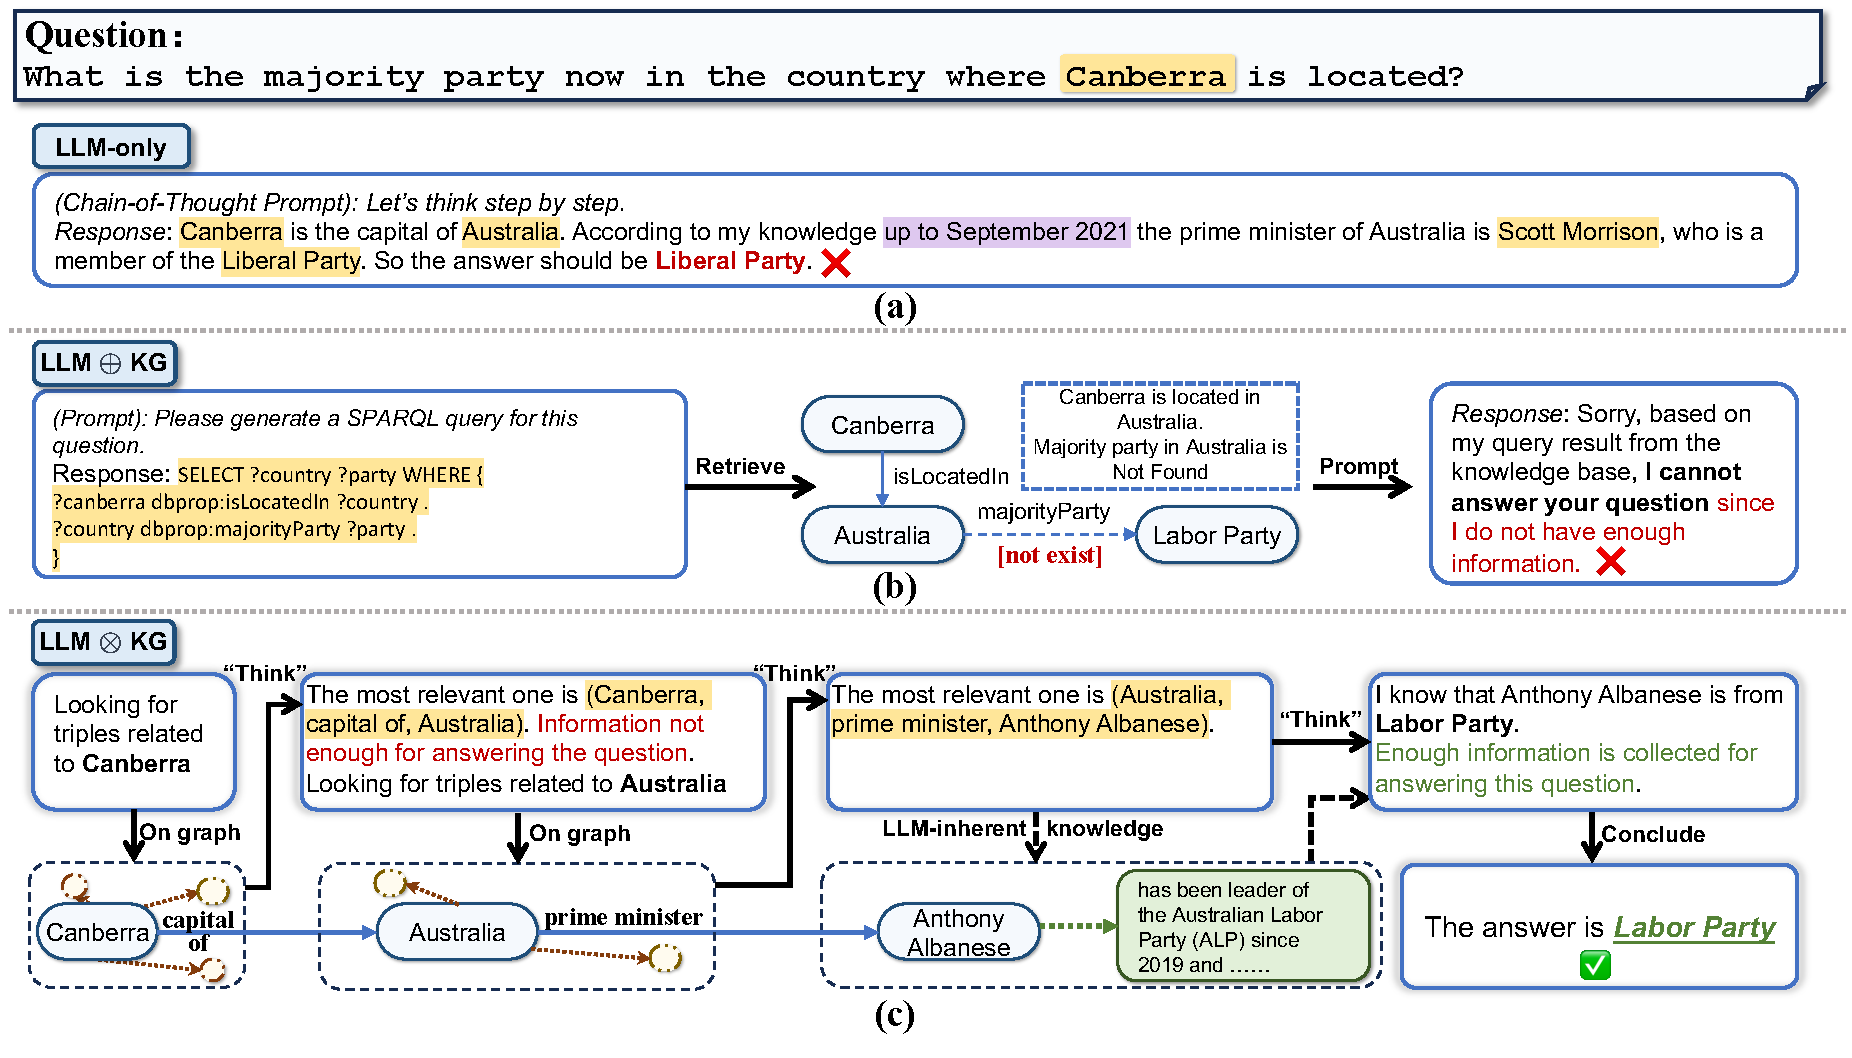
\includegraphics[width=0.95\columnwidth]{img/fig1_v2.pdf}
 \caption{Representative workflow of three LLM reasoning paradigms: (a) LLM-only (e.g., Chain-of-Thought prompting), (b) LLM $\oplus$ KG (e.g., KBQA via LLM-generated SPARQL query), (c) LLM $\otimes$ KG (e.g., Think-on-Graph).}
	% \caption{Comparisons of the reasoning processes of Chain-of-Thought prompting (top), knowledge reasoning based on ``$\hbox{LLM}\oplus\hbox{KG}$'' (middle), and ``$\hbox{LLM}\otimes\hbox{KG}$'' (bottom).}
         \vspace{-10pt}
	\label{fig: example}
\end{figure}

% To overcome these challenges, one promising approach involves integrating LLMs with external knowledge sources to serve as references for generating responses. For instance, researchers have explored incorporating information from web pages \citep{web, verifyandedit} or knowledge graphs \citep{cok, skg, knowledgeaugmented, yang2023chatgpt, wang2023boosting} and adapting prompts accordingly to mitigate hallucination in LLMs. These methods have effectively enhanced LLMs' performance on knowledge-intensive tasks by supplementing them with additional information. However, these approaches usually suffer from certain limitations when faced with complicated questions.
% Firstly, the constraints on the input length of LLMs hinder the inclusion of more comprehensive information through prompts.
% Besides, previous approaches that combined retrieval and external knowledge integration overlook the "deep" reasoning capability of LLMs.
% Recent studies \citep{COT, auto, zeroshot, SC, iter-cot} have demonstrated that LLMs can enhance their performance by generating intermediate reasoning steps and leveraging task-specific examples as demonstrations to perform complexa promising complement to the drawbacks of LLMs multi-hop reasoning.

Recognizing these challenges, a natural and promising solution is to incorporate external knowledge such as knowledge graphs (KGs) to help improve LLM reasoning.
KGs offer structured, explicit, and editable representations of knowledge, presenting a complementary strategy to mitigate the limitations of LLMs \citep{pan2023unifying}.
% KGs provide structured, explicit and editable knowledge representations, thus being considered as a promising complement to the drawbacks of LLMs \citep{pan2023unifying}.
Researchers \citep{cok, skg, knowledgeaugmented, yang2023chatgpt, wang2023boosting, structgpt} have explored the usage of KGs as external knowledge sources to mitigate hallucination in LLMs. These approaches follow a routine: retrieve information from KGs, augment the prompt accordingly, and feed the increased prompt into LLMs (as illustrated in Figure \ref{fig: example}b). In this paper, we refer to this paradigm as ``$\hbox{LLM}\oplus\hbox{KG}$''.
Although aiming to integrate the power of LLM and KG, in this paradigm, LLM plays the role of translator which transfers input questions to machine-understandable command for KG searching and reasoning, but it does not participate in the graph reasoning process directly. Unfortunately, the loose-coupling $\hbox{LLM}\oplus\hbox{KG}$ paradigm has its own limitations, and its success depends heavily on the completeness and high quality of KG. In Figure \ref{fig: example}b, for example, although LLM successfully identified necessary relation types required to answer the question, the absence of the relation ``majority party'' leads to a failure in retrieving the correct answer.


%While in this paradigm the KG and LLM provides supplementary/complementary abilities to each other, the clear boundary of their duties (LLM as info translator and KG as info provider) hinders the comprehensive/omni-?/finer-granularity integration/cooperation between these two parts, resulting in limited synergistic effect of this combination. For example, in Figure \ref{fig: example}b, the wide-reaching connections in KG allows an alternative path (Figure \ref{fig: example}c) to the answer the question although the direct relation type does not exist. However, the derivation of this alternative path relies on the dynamic reasoning and interactive decision-making capabilities inherent to LLM agents \citep{yao2022react}, which requires finer-granular KG-LLM interaction.

%However, these methods often do not fully harness the advantages of KGs, such as their wide-reaching connections (for instance, in Figure \ref{fig: example}b, the missing relation "majority party" can be supplemented by an alternative path in Figure \ref{fig: example}c) and the dynamic reasoning and interactive decision-making capabilities inherent to LLM agents \citep{yao2022react} (as exemplified by the reasoning path in Figure \ref{fig: example}c). Hence, they may underutilize the synergistic strength of LLMs and KGs.

% However, these approaches usually overlook the advantages of KGs in terms of ubiquitous connectivity (e.g. the non-existing relation ``majority party'' in middle Figure \ref{fig: example} can be complemented by the alternative path in the bottom) and the dynamic reasoning and interactive decision-making capabilities of LLMs (coming up with the reasoning path in Figure \ref{fig: example}), thereby failing to complement the strengths of LLMs and KGs.
% Due to the connectivity of KGs, there are also some approaches \citep{kg_beam, kg_dfs} based on semantic parsing that employ graph search algorithms such as beam search \citep{beamsearch} and depth-first search (DFS). Moreover, prior studies \citep{tot, beamsearchqa, self_eval} have demonstrated that LLMs can enhance their reasoning performance by employing algorithms based on constrained search methods. Some studies 

Building upon these considerations, we propose a new tight-coupling ``$\hbox{LLM} \otimes \hbox{KG}$'' paradigm where KGs and LLMs work in tandem, complementing each other's capabilities in each step of graph reasoning.
Figure \ref{fig: example}c provides an example illustrating the advantage of $\hbox{LLM} \otimes \hbox{KG}$. In this example, the missing relation "majority party" resulting in the failure in Figure \ref{fig: example}b can be complemented by a reference triple $(\textbf{Australia},\textbf{prime minister},\textbf{Anthony Albanese})$ discovered by the LLM agent with dynamic reasoning ability \citep{yao2022react}, as well as the political party membership of \textbf{Anthony Albanese} coming from LLM's inherent knowledge.
% by an alternative reasoning path (Australia $\xrightarrow{\text{prime minister}}$ Anthony Albanese $\xrightarrow{\text{member of}}$ Labor Party) discovered by LLM, 
%thanking the dynamic decision-making capability and inherent knowledge of LLM .
In this way, the LLM succeeds in generating the correct answer with reliable knowledge retrieved from KGs.
% (LLMs generate query/response sentence and KGs execute in Figure \ref{fig: example}b).
As an implementation of this paradigm, we propose an algorithmic framework ``Think-on-Graph'' (meaning: LLMs ``Think'' along the reasoning paths ``on'' knowledge ``graph'' step-by-step, abbreviated as ToG below),
% which is essentially an autonomous LLM-based agent system \citep{yao2022react}
for deep, responsible, and efficient LLM reasoning.
Using the beam search algorithm \citep{beamsearch} in KG/LLM reasoning \citep{kg_beam, beamsearchqa, self_eval, liu2024what}, ToG allows LLM to dynamically explore a number of reasoning paths in KG and make decisions accordingly.
Given an input question, ToG first identifies initial entities and then iteratively calls the LLM to retrieve relevant triples from KGs through exploration (looking for relevant triples in KG via ``on graph'' step) and reasoning (deciding on the most relevant triples via ``think'' step) until adequate information through the top-N reasoning paths in beam search is gathered to answer the question (judged by LLMs in "Think" step) or the predefined maximum search depth is reached.

%This process produces multiple high-probability reasoning paths comprised of sequentially connected triples and persists until adequate information is gathered to answer the question (judged by LLMs in "Think" step) or the predefined maximum depth is reached.

% By following this procedure, we can substantially improve the factual reasoning capabilities of LLMs, effectively mitigating hallucination issues and enhancing response precision.

% This process generates multiple high-probability reasoning paths consisting of sequentially connected triples and continues until sufficient information is acquired to answer the question or the maximum depth is reached.
% Following this procedure, we can significantly enhance the factual reasoning capabilities of LLMs, thus effectively mitigating hallucination issues and improving response precision.
% regards the dynamic combination of KGs and LLMs as an agent system.

% \citet{yao2022react} have demonstrated the feasibility of utilizing LLMs as agents to autonomously interact with external environment and make decisions, thereby improving the effectiveness, interpretability and trustworthiness of LLMs' reasoning processes. Motivated by this, we propose a new paradigm, ``$\hbox{LLM}\otimes \hbox{KG}$'', which regards the dynamic combination of KGs and LLMs as an agent system. The KGs play the role of a responsible environment and LLMs perform graph exploration as agents. 

% Inspired by the success of the beam search algorithm \citep{beamsearch} in KG reasoning \citep{kg_beam} and LLM reasoning \citep{beamsearchqa, self_eval}, we introduce the Think-on-Graph (ToG) framework on the top of ``$\hbox{LLM}\otimes \hbox{KG}$'', which leverages the LLM to dynamically explore the limited number of reasoning paths on the KG and make decisions accordingly. 
% % Building upon the preceding conclusions, and the necessity for deep and responsible reasoning, we introduce the Think-on-Graph (ToG) framework which leverages factual knowledge to drive the step-by-step thinking of LLMs.
% Specifically, given an input question, ToG first identifies topic entities and then leverages an LLM to iteratively retrieve relevant triples from KGs through iterative exploration and reasoning. 
% This iterative search process generates multiple high-probability reasoning paths consisting of sequentially connected triples, and continues until sufficient information is acquired to answer the question or the maximum depth is reached.
% Following this procedure, we can significantly enhance the factual reasoning capabilities of LLMs, thus effectively mitigating hallucination issues and improving response precision.

% To illustrate, consider the question "What is the majority party now in the country where Caberra is located?" depicted in Figure \ref{fig: example}. When employing chain-of-thought reasoning alone, the process may be conceptually correct but prone to erroneous results due to out-of-date knowledge (hallucination).  ``$\hbox{LLM}\oplus\hbox{KG}$'' approaches, on the other hand, are limited by incompleteness of KG and might fail in knowledge retrieval, e.g., missing the "majority party" relation in this case. In contrast, ToG employs a LLM to alternately conduct graph exploration and reasoning on KGs to dynamically generate reasoning paths,  which effectively address intricate questions by leveraging the interpretive capacity of LLMs and integrating the strengths of KGs.

%We evaluate ToG on various knowledge-intensive tasks, including knowledge base QA (KBQA), open-domain QA, slot filling and fact checking.
The advantage of ToG can be abbreviated as
(1) \textbf{Deep reasoning:}
ToG extracts diverse and multi-hop reasoning paths from KGs as the basis for LLM reasoning, enhancing LLMs' deep reasoning capabilities for knowledge-intensive tasks.
% ToG demonstrates favorable performance in various multi-hop reasoning tasks (Section \ref{sec:main_results}), with performance improvements generally becoming greater as the depth of reasoning increases (Figure \ref{fig: right_proportion}).
(2) \textbf{Responsible reasoning:}
Explicit, editable reasoning paths improve the explainability of the reasoning process of LLMs, and enable the tracing and correction of the provenances of models' outputs.
% ToG induces explicit and modifiable reasoning paths that enhance the transparency of LLMs' reasoning processes, facilitating the tracking and rectification of model output origins (Section \ref{sec: application}).
(3) \textbf{Flexibility and efficiency:}
a) ToG is a plug-and-play framework that can be applied to a variety of LLMs and KGs seamlessly.
b) Under ToG framework, knowledge can be updated frequently via KG instead of LLM whose knowledge-update is expensive and slow.
c) ToG enhances the reasoning ability of small LLMs (e.g., LLAMA2-70B) to be competitive with big LLMs (e.g., GPT-4).
% ToG serves as a plug-and-play, training-free framework applicable to various LLMs and KGs. It harnesses the strengths of KGs to effectively address the challenge of knowledge update in LLMs, empowering billion-scale LLMs (Llama2) to outperform trillion-scale LLMs (GPT-4) in knowledge reasoning capabilities (Section \ref{sec:backbone}).

% In summary, ToG addresses the inherent limitations of LLMs in three aspects:
% \item \textbf{Deep Reasoning:}  ToG extracts diverse and multi-hop reasoning paths from KGs as the basis for LLM reasoning, enhancing LLMs' deep reasoning capabilities for knowledge-intensive tasks.
% \item \textbf{Responsibility:} Explicit, editable reasoning paths improve the explainability of the reasoning process of LLMs, and enable the tracing and correction of the provenances of models' outputs.
% \item \textbf{Efficiency:}  ToG is a plug-and-play framework that can be applied to a variety of LLMs and KGs without training. ToG leverages the benefits of KGs to efficiently solve the knowledge-updating problem of LLMs and empower billion-scale LLMs (LLAMA2) to have stronger knowledge reasoning capabilities than trillion-scale LLMs (GPT4).

% Furthermore, we analyze how ToG can substantially alleviate the hallucination issue, as shown in Section \ref{sec: analysis}.

%%%我们的贡献有三点：1. ToG从KG中抽取多样性的复杂知识链作为大语言模型的推理依据，有效地决知识密集的深度推理问题。2. 显示的，可编辑的知识链提高了大语言模型推理过程的可解释性，并使得生成内容可以溯源和修正. 3. ToG是一个即插即用的技术，可以在不经过训练的情况下适用于各种大语言模型和知识图谱。可以利用知识图谱有效率地解决大语言模型的知识更新问题，并使轻量级的大语言模型具有强大的知识推理能力。
% In summary, ToG addresses the inherent limitations of LLMs in three aspects:
% \begin{itemize}[leftmargin=*]
% \item \textbf{Deep Reasoning:} ToG demonstrates favorable performance in various multi-hop reasoning tasks (Section \ref{sec:main_results}), with performance improvements generally becoming greater as the depth of reasoning increases (Figure \ref{fig: right_proportion}).
% \item \textbf{Responsibility:} ToG induces explicit and modifiable reasoning paths that enhance the transparency of LLMs' reasoning processes, facilitating the tracking and rectification of model output origins (Section \ref{sec: application}).
% \item \textbf{Efficiency:} ToG serves as a plug-and-play, training-free framework applicable to various LLMs and KGs. It harnesses the strengths of KGs to effectively address the challenge of knowledge update in LLMs, empowering billion-scale LLMs (Llama2) to outperform trillion-scale LLMs (GPT-4) in knowledge reasoning capabilities (Section \ref{sec:backbone}).

% \end{itemize}


\begin{figure}[t]
	\centering
	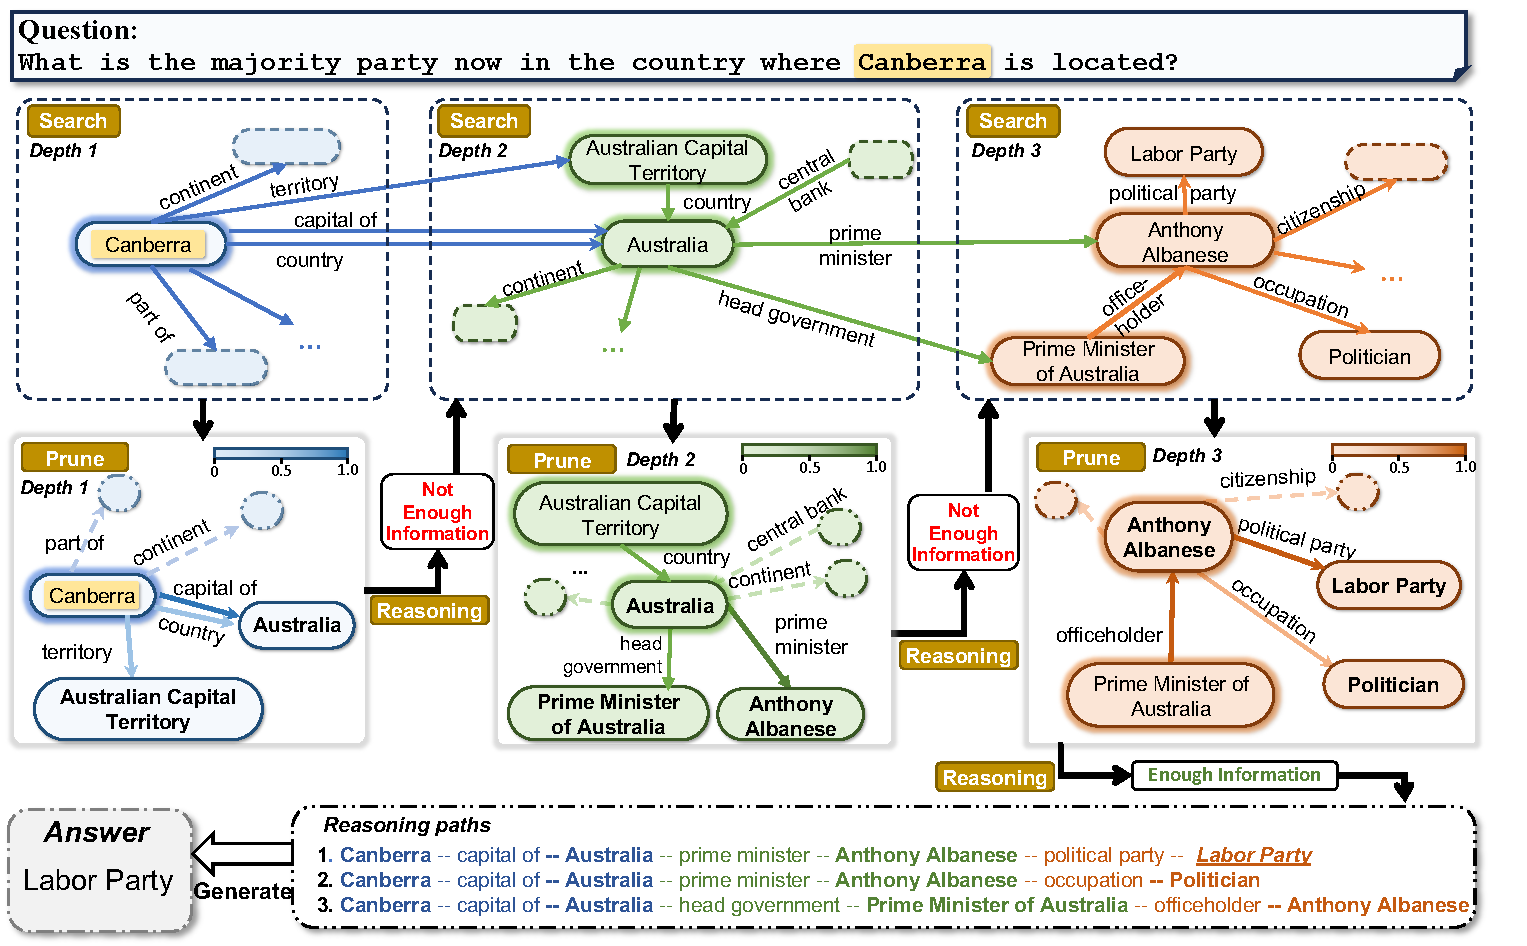
\includegraphics[width=0.95\columnwidth]{img/fig2.pdf}
	\caption{An example workflow of ToG. The glowing entities are the central entities where the search starts at each iteration (depth), and the entities with \textbf{boldface} are the selected central entities for the next iteration after pruning. At each pruning step, the darkness of the edges represents the ranking score given by LLM, and the dashed lines indicate relations that have been pruned due to low evaluation scores.}
         % \vspace{-10pt}
	\label{fig: framework}
\end{figure}

\section{Methods}
\label{sec: methods} 
ToG implements the ``$\hbox{LLM}\otimes \hbox{KG}$'' paradigm by asking LLM to perform beam search on knowledge graph. Specifically, it prompts the LLM to iteratively explore multiple possible reasoning paths on KGs until the LLM determines that the question can be answered based on the current reasoning paths. ToG constantly updates and maintains top-$N$ reasoning paths $P=\{p_1,p_2,\ldots, p_N\}$ for the question $x$ after each iteration, where $N$ denotes the width of beam search.
% Each path $p_n$ consists of $D$ triples $p_n =\{(e^d_{s,n}, r^d_{j,n}, e^d_{o,n})\}^{D}_{d=1}$, where $e^d_{s,n}$ and $e^d_{o,n}$ denote subject and object entities, $r^d_{j,n}$ is a specific relation between them, $(e^d_{s,n}, r^d_{j,n}, e^d_{o,n})$ and $(e^{d+1}_{s,n}, r^{d+1}_{j,n}, e^{d+1}_{o,n})$ are connected to each other, and $D$ denotes the current iteration depth. The sets of the tail entities and relations in $P$ are denoted as $E^{D}=\{e^{D}_{1},e^{D}_{2},...,e^{D}_{N}\}$ and $R^{D}=\{r^{D}_{1},r^{D}_{2},...,r^{D}_{N}\}$, respectively. 
The entire inference process of ToG contains the following 3 phases: initialization, exploration, and reasoning. 
% In particular, we propose a variant of ToG, relation-based ToG by exploring top-$N$ relations chains $p_n = (e^{0}_n,r^{1}_n,r^{2}_n,...,r^{D}_n)$ starting with the topic entity $e^{0}_n$, instead of triple-based reasoning paths.

\subsection{Think-on-Graph}

\subsubsection{Initialization of Graph Search}
% Denote the sets of the tail entities and relations in $P$ as $E^{D}=\{e^{D}_{1},e^{D}_{2},...,e^{D}_{N}\}$ and $R^{D}=\{r^{D}_{1},r^{D}_{2},...,r^{D}_{N}\}$. 
Given a question, ToG leverages the underlying LLM to localize the initial entity of the reasoning paths on knowledge graph. This phase can be regarded as the initialization of the top-$N$ reasoning paths $P$. ToG first prompts LLMs to automatically extract the topic entities in question and gets the top-$N$ topic entities $E^{0}=\{e^{0}_{1},e^{0}_{2},...,e^{0}_{N}\}$ to the question. Note that the number of topic entities might possibly be less than $N$.

\subsubsection{Exploration}
At the beginning of the $D$-th iteration, each path $p_n$ consists of $D-1$ triples, i.e., $p_n =\{(e^d_{s,n}, r^d_{j,n}, e^d_{o,n})\}^{D-1}_{d=1}$, where $e^d_{s,n}$ and $e^d_{o,n}$ denote subject and object entities, $r^d_{j,n}$ is a specific relation between them, $(e^d_{s,n}, r^d_{j,n}, e^d_{o,n})$ and $(e^{d+1}_{s,n}, r^{d+1}_{j,n}, e^{d+1}_{o,n})$ are connected to each other. The sets of the tail entities and relations in $P$ are denoted as $E^{D-1}=\{e^{D-1}_{1},e^{D-1}_{2},...,e^{D-1}_{N}\}$ and $R^{D-1}=\{r^{D-1}_{1},r^{D-1}_{2},...,r^{D-1}_{N}\}$, respectively. 

The exploration phase in the $D$-th iteration aims to exploit the LLM to identify the most relevant top-$N$ entities $E^{D}$ from the neighboring entities of the current top-$N$ entity set $E^{D-1}$ based on the question $x$ and extend the top-$N$ reasoning paths $P$ with $E^{D}$.
To address the complexity of handling numerous neighboring entities with the LLM, we implement a two-step exploration strategy: first, exploring significant relations, and then using selected relations to guide entity exploration.
%based on a given to serve as intermediate steps in the reasoning paths for a given question based on \textbf{Beam Search}. This phase comprises two distinct stages: relation exploration and entity exploration.  %%为什么要分为两步，一个是因为 下一步的实体candidate数量很多，分两步搜索可以减少单次搜索的宽度

% The set of $E_c$ entities at the current search depth $D_c$, $\{t_i\}^{N}_{i=1} \sim $\text{take}(N)($p_\theta(t_{m+1} | x, E_c) = p_\theta(t_{m+1} | x, \{(e_s, r_j, e_o)\}^{D}_{j=1})), t_i = (e_s, r_i, e_o) $. 



\paragraph{Relation Exploration}
\label{sec: relation_exploration}
Relation exploration is a beam search process with the depth of 1 and the width of $N$ from $E^{D-1}$ to $R^{D}$. 
%For each path $p_n$ of the current top-$N$ reasoning paths $P$, we expand $p_n$ with new candidate tail relations $R^{D}_{cand,n}$. And then we use the LLM to select out new top-$N$ reasoning paths $P$ ending with $R^{D}$ from all candidate reasoning paths $P_{cand}$. 
The whole process can be decomposed into two steps: \texttt{Search} and \texttt{Prune}. The LLM serves as an agent to automatically complete this process.
\begin{itemize}[leftmargin=*]
%%应该是参考图例，进行清晰地描述：第一步是searches all the relations
    % \item \textbf{Search} The relation exploration phase first searches all the relations $R_{cand} = \{R_s \cup R_o\}$, where $R_s$ and $R_o$ denote the relation edge set with the current entity as the subject or object entity, respectively, linked to each entity in the current entity set $E_{c}$, where $E_{c}$ of the first iteration is initialized by $E_{init}$, and subsequent $E_c$ updated after each iteration. The same applies to the set of current scores $S_c$. The \texttt{Search} procedure can be easily completed by executing two simple pre-defined formal queries, which makes ToG adapt well to different KBs.


    
    \item \textbf{Search} 
    % At the beginning of the $i$-th iteration, for each current reasoning path $p_j$ where $j\in(1，N)$, the relation exploration phase first search out relations $R^{i}_{cand,j}$ linked to the tail entity of $p_j$. Specially for the first iteration where $P$ is initialized by $E_{init}$. In the case of Figure~\ref{fig: framework}, $E^{1}_c=\{\textbf{Canberra}\}$ and $R_{cand}$ denotes the set of all relations linked to \textbf{Canberra} inwards or outwards when \textit{Depth} = 1. After the first iteration, $E^{i}_c$. The \texttt{Search} procedure can be easily completed by executing two simple pre-defined formal queries, which makes ToG adapt well to different KBs \textbf{without any training cost}.
    At the beginning of the $D$-th iteration, the relation exploration phase first searches out relations $R^{D}_{cand,n}$ linked to the tail entity $e^{D-1}_{n}$ for each reasoning path $p_n$. These relations are aggregated into $R^{D}_{cand}$. In the case of Figure~\ref{fig: framework}, $E^{1}=\{\textbf{Canberra}\}$ and $R^{1}_{cand}$ denotes the set of all relations linked to \textbf{Canberra} inwards or outwards. Notably, the \texttt{Search} procedure can be easily completed by executing two simple pre-defined formal queries shown in Appendix~\ref{sparqls} and~\ref{APIs}, which makes ToG adapt well to different KGs \textbf{without any training cost}.
    
    \item \textbf{Prune} Once we have obtained the candidate relation sets $R^{D}_{cand}$ and the expanded candidate reasoning paths $P_{cand}$ from the relation search, we can utilize the LLM to select out new top-$N$ reasoning paths $P$ ending with the tail relations $R^{D}$ from $P_{cand}$ based on the literal information of the question $x$ and the candidate relations $R^{D}_{cand}$. The prompt used here can be found in Appendix~\ref{prompts4rel}. 
    %we prune relations that have a low contribution to the question and as the termination for the current relation exploration phase. 
    % Since $r\in R^{D}_{cand,n}$ is expressed in natural language, we can utilize the LLM to select the most relevant top-$N$ relations $R^{D}_{c,n}=\{r^{D}_{c,n,i}\}^{N}_{i=1}$ for each candidate set $R^{D}_{cand,n}$ with their corresponding scores $\{s^{D}_{r,n,i}\}_{i=1}^{N}$, based on their relevance to the question and the reasoning path $p_n$. 
    As shown in Figure~\ref{fig: framework}, the LLM selects top-3 relations $\{\textbf{capital of}, \textbf{country}, \textbf{territory}\}$ out from all relations linked to the entity \textbf{Canberra} in the first iteration. Since \textbf{Canberra} is the only topic entity, the top-3 candidate reasoning paths are updated as $\{(\textbf{Canberra, capital of})$, $(\textbf{Canberra, country})$,$(\textbf{Canberra, territory})\}$.
        % with the corresponding scores as our current relation set $ R_{c} = \{(r_{i}, s_{i})\}_{i=1}^{N}, s.t. \sum_{i=1}^{N} s_{i} = 1, s_{i} = p_{\theta}(r_{i}|x, e_{j}), r_{i} \in R_{cand}, e_{j} \in E_{c}$. Then, we update and normalize the scores $ S_c = \left\{ \frac{s_{S_c}^{i} \cdot s_{R_c}^{i}}{\sum_{j=1}^{n} s_{S_c}^{j} \cdot s_{R_c}^{j}} \right\}_{i=1}^{n}$, where $s_{S_c}^{i}$ and $s_{R_c}^{i}$ denote the $i-th$ scores of the $S_c$ and $R_c$ sets, respectively.

        
        % $S_c = Normalize(\{s_{S_c}^{i} \cdot s_{R_c}^{i}\}_{i=1}^{n})$, where $s_{S}^{i}$ denotes the $i-th$ score of the $S$.
%  = p_{\theta}(r_{i}|x, E_{c})
% $R_{c} = \{p_\theta(r_i|x, E_c)\}^{N}_{i=1} = \{p_\theta(r_i|x, e_j)\}^{N}_{i=1}, r_i \in R_{cand}, e_j \in E_c$. 
\end{itemize}

\paragraph{Entity Exploration}
\label{sec: entity_exploration}
Similar to relationship exploration, entity exploration is also a beam search process performed by the LLM from $R^{D}$ to $E^{D}$, and consists of two steps, \texttt{Search} and \texttt{Prune}.
\begin{itemize}[leftmargin=*]
    \item \textbf{Search} Once we have obtained new top-$N$ reasoning paths $P$ and the set of new tail relations $R^{D}$ from relation exploration, for each relation path $p_n\in P$, we can explore a candidate entity set $E^{D}_{cand,n}$ by querying $(e^{D-1}_n, r^{D}_n,?)$ or $(?, r^{D}_n,e^{D-1}_n)$, where $e^{D-1}_n, r_n$ denote the tail entity and relation of $p_n$. We can aggregate $\{E^{D}_{cand,1},E^{D}_{cand,2},...,E^{D}_{cand,N}\}$ into $E^{D}_{cand}$ and expand top-$N$ reasoning paths $P$ to $P_{cand}$ with the tail entities $E^{D}_{cand}$.
    % the entity set $E^{i}_c$ and its corresponding relation set $R^{i}_{c}$ for the $i$-th iteration, we can explore N candidate entity sets  $E^{i}_{cand} = \{e_m|E_c, R_{c}\}_{i=1}^{D} = \{\{\{e_m|e_j, r_k\}_{k=1}^{N}\}_{j=1}^{L}\}_{m=1}^{D}$ by querying $(e_j, r_k,?)$ or $(?, r_k,e_j)$, where $e_j \in E_c, r_k \in R_{c}$, $N$, $L$ and $D$ denotes the size of $R_{c}$, $E_c$ and $E_{cand}$, respectively. 
    For the shown case, $E^{1}_{cand}$ can be represented as  $\{\textbf{Australia},\textbf{Australia}, \textbf{Australian Capital Territory}\}$.
    \item \textbf{Prune} Since the entities in each candidate set $E^{D}_{cand}$ is expressed in natural language, we can leverage the LLM to select new top-$N$ reasoning paths $P$ ending with the tail entities $E^{D}$ out from $P_{cand}$. The prompt used here can be found in Appendix~\ref{prompts4ent}. As shown in Figure~\ref{fig: framework}, \textbf{Australia} and \textbf{Australian Capital Territory} are scored as 1 since the relations \textbf{capital of}, \textbf{country} and \textbf{territory} are only linked to one tail entity respectively, and the current reasoning paths $p$ are updated as $\{(\textbf{Canberra, capital of, Australia}),(\textbf{Canberra, country, Australia})$, $(\textbf{Canberra, territory, Australian Capital Territory})\}$.
    % \item \textbf{Prune} Since the candidate set $E_{cand}$ is still expressed in natural language, we leverage the LLM to prune the candidate entity set $E^{i}_c$ based on the query to obtain the most relevant top-$N$ entities $E_{N} = \{(e_{i}, s_{i})\}_{i=1}^{N}, s.t. \sum_{i=1}^{N} s_{i} = 1, s_{i} = \{p_\theta(e_i|x, e_j, r_k)\}^{N}_{i=1}, e_i \in E_{cand}, e_j \in E_c$, $r_k \in R_c$. Then, we also update the and normalize scores $ S_c = \left\{ \frac{s_{S_c}^{i} \cdot s_{E_N}^{i}}{\sum_{j=1}^{n} s_{S_c}^{j} \cdot s_{E_N}^{j}} \right\}_{i=1}^{n}$.
    
%$S_c = Normalize(\{s_{S_c}^{i} \cdot s_{E_N}^{i}\}_{i=1}^{n})$.
% \{p_\theta(e_i|x, E_c, R_c)\}^{N}_{i=1} =
% $E_{N} = \{p_\theta(e_i|x, E_c, R_c)\}^{N}_{i=1} = \{p_\theta(e_i|x, e_j, r_k)\}^{N}_{i=1}, e_i \in E_{cand}, e_j \in E_c$, $r_k \in R_c$.
\end{itemize}
After executing the two explorations described above, we reconstruct new top-$N$ reasoning paths $P$ where the length of each path increases by 1. Each prune step requires at most $N$ LLM calls.
%We then \textbf{update} the $E_c$ with $E_N$ to continue the iteration process. Finally, we can construct a comprehensive reasoning path where each intermediate step corresponds to a triple that is sequentially related.
% and calculate $S_c = \{s_{S_c}^{i} \cdot s_{R_c}^{i} \cdot s_{E_N}^{i}\}_{i=1}^{n}$, where $s_{S}^{i}$ denotes the score of the $i-th$ entity of the current$S$, 
\subsubsection{Reasoning}
\label{sec: reasoning}
Upon obtaining the current reasoning path $P$ through the exploration process, we prompt the LLM to evaluate whether the current reasoning paths are adequate for generating the answer. If the evaluation yields a positive result, we prompt the LLM to generate the answer using the reasoning paths with the query as inputs as illustrated in Figure~\ref{fig: framework}. The prompt used for evaluation and generation can be found in Appendix~\ref{prompts4rea} and~\ref{prompts4gen}. Conversely, if the evaluation yields a negative result, we repeat the \texttt{Exploration} and \texttt{Reasoning} steps until the evaluation is positive or reaches the maximum search depth $D_{max}$. If the algorithm has not yet concluded, it signifies that even upon reaching the $D_{max}$, ToG remains unable to explore the reasoning paths to resolve the question. In such a scenario, ToG generates the answer exclusively based on the inherent knowledge in the LLM.
The whole inference process of ToG contains $D$ exploration phases and $D$ evaluation steps as well as a generation step, which needs at most $2ND+D+1$ calls to the LLM. 


\subsection{Relation-based Think-on-Graph}

% \subsubsection{Exploration}
% The exploration phase is divided into two parts: Search and Prune. It is important to note that the relation exploration is similar to that of entity based approach, 
% \paragraph{Relation Exploration}
 %ToG(E)存在哪些问题：，Unameuntity。我们又发现，在不完备的kb中，关系的信息比实体要重要\ref{3.4.2}.然后我们提出relation。，这个东西focus on bala，在不完备的kb上飙戏那更好。整体pipeline，这两个方法一样，只不过有两点有些区别。
Previous KBQA methods, particularly based on semantic parsing, have predominantly relied on relation information in questions to generate formal queries~\citep{complexKBQA}. Inspired by this, we propose relation-based ToG (ToG-R) that explores the top-$N$ relation chains $\{p_n = (e^{0}_n,r^{1}_n,r^{2}_n,...,r^{D}_n)\}^N_{n=1}$ starting with the topic entities $\{e^{0}_n\}^N_{n=1}$ instead of triple-based reasoning paths. ToG-R sequentially performs \text{relation search}, \text{relation prune} and \text{entity search} in each iteration, which is the same as ToG. Then ToG-R performs the \text{reasoning} step based on all candidate reasoning paths ending with $E^{D}_{cand}$ obtained by entity search. If the LLM determines that the retrieved candidate reasoning paths do not contain enough information for the LLM to answer the question, we randomly sample N entities from the candidate entities $E^{D}_{cand}$ and continue to the next iteration. Assuming that entities in each entity set $E^{D}_{cand,n}$ probably belong to the same entity class and have similar neighboring relations, the results of pruning the entity set $\{E^{D}_{cand,n}\}^N_{n=1}$ might have little impact on the following relation exploration. Thus, we use the random beam search instead of the LLM-constrained beam search in ToG for \text{entity prune}, referred to as \textbf{random prune}. Algorithm \ref{algorithm1} and \ref{algorithm2} show the implementation details of the ToG and ToG-R. ToG-R needs at most $ND+D+1$ calls to the LLM.
% ToG-R traverses entities, converting all intermediate steps into relations, and generates answers based on candidate entity sets corresponding to the complete reasoning chains.
% It leverages LLMs' reasoning capabilities to generate answers using different candidate sets for each chain in the reasoning process. 



% Notably, both approaches follow similar pipelines but differ in extending the reasoning chains in the intermediate steps.




%\subsubsection{Reasoning}
% Relation-based ToG also performs esolely involves the relation exploration phase and the reasoning phase. The relation exploration remains unchanged, and the reasoning phase consists of two steps: The generation of relations through a two-step approach, \texttt{Search} and \texttt{Prune}.


% \begin{itemize}[leftmargin=*]
%     \item \textbf{Entity Search} Once the top-$N$ reasoning paths $P$ are updated with new tail relations by relation exploration, The samples in $E^{D-1}_c$ are independently and identically distributed, and through the calculation of the averages of several samples, we can derive the mean of the relations $R^{D}_{cand}$ within $E^{D-1}_c$. Specifically, we randomly sample N entities based on the $E^{D-1}_{c}$, and search the relations in both directions as $R_{cand}$ and prune to $R^{D}_{c}$, in the same way as Section \ref{sec: relation_exploration}.
%     \item \textbf{Path-aware Entity Search} As the intermediate steps do not involve any entities, we need to obtain $E^{D}_{cand}$ based on $R^{D}_c$, history paths $P$ and $E_{c}$, where $E_c$ is fixed. Accordingly, $E_{cand}$ serves as the terminal node in the reasoning paths, illustrated in Table \ref{table: case3}.

% \end{itemize}

Compared to ToG, ToG-R offers two key benefits: 1) It eliminates the need for the process of pruning entities using the LLM, thereby reducing the overall cost and reasoning time. 2) ToG-R primarily emphasizes the literal information of relations, mitigating the risk of misguided reasoning when the literal information of intermediate entities is missing or unfamiliar to the LLM. 


% \subsection{Generate Reasoning State}
% The current reasoning state is denoted as $s$, representing a retrieved triple $t_i = (e_s, r_i, e_o)$. Based on the characteristics of triples, we initially search for the corresponding relation and subsequently search for the head entity and tail entity (or tail entity and head entity) based on the directionality of the relation.

% \subsubsection{Retrieve and Rank Relations}
% After obtaining the initial entity set and contribution degree for each entity in the set, we must execute SPARQL to retrieve all relationships in the knowledge graph related to the entity (both as a subject and object) as $R_{all} = \{R_s, R_o\}$. These relationships must then be sorted. As relationships in the knowledge graph exist in natural language, we can use LLMs to assign a related score to each relationship based on its name. Finally, the topN relationships based on their scores must be retained.

% \subsubsection{Retrieve and Rank Entities}
% Upon obtaining the corresponding relationships for each entity in the previous step, we can retrieve the tail entity (or head entity, depending on the direction of the relationship) using SPARQL, and construct a triple. By iteratively performing the second and third steps, we can obtain multiple triples where the head and tail entities are interrelated. In this way, we express a reasoning path through triples.
% \subsection{Evaluate Paths}
% Given a retrieved reasoning chain, we prompt LLMs to automatically determine whether the current chain provides sufficient knowledge to answer the question or whether the search path has reached a pre-designed threshold.
% \subsection{Search algorithm}
% Unlike ToT \citep{tot}, our initial state is a set of identified entities, so we use \textbf{Breadth-first Search (BFS)}. For each entity in the initial state, we search simultaneously and always maintain a top-$N$ reasoning chain based on scores.
\section{Experiments}
\label{sec: experiments}
\subsection{Experimental Design}
\subsubsection{Datasets and Evaluation Metrics}
\label{sec: datasets}
In order to test ToG's ability on multi-hop knowledge-intensive reasoning tasks, we evaluate ToG on five KBQA datasets (4 Multi-hop and 1 Single-hop): CWQ \citep{cwq_dataset}, WebQSP \citep{webqsp_dataset}, GrailQA \citep{garilqa_dataset}, QALD10-en \citep{qald10-en_dataset}, Simple Questions \citep{simple_questions_dataset}. Moreover, in order to examine ToG on more generic tasks, we also prepare one open-domain QA dataset: WebQuestions \citep{webq_dataset}; two slot filling datasets: T-REx \citep{trex_dataset} and Zero-Shot RE \citep{kilt}; and one fact-checking dataset: Creak \citep{creak_dataset}. 
Note that, for two big datasets GrailQA and Simple Questions, we only randomly selected 1,000 samples each for testing in order to save computational cost. 
For all datasets, exact match accuracy (Hits@1) is used as our evaluation metric following previous works \citep{cok, knowledgeaugmented, structgpt, DB-BLINDER}.


\begin{table}[t]
\centering
\renewcommand{\arraystretch}{1.3}
\resizebox{\linewidth}{!}{
\begin{tabular}{lccccccccc}
\toprule
\multirow{2}{*}{Method}
     & \multicolumn{4}{c}{Multi-Hop KBQA} & Single-Hop KBQA & Open-Domain QA & \multicolumn{2}{c}{Slot Filling} & Fact Checking \\ 
     \cmidrule(r){2-5}  \cmidrule(r){6-6} \cmidrule(r){7-7} \cmidrule(r){8-9} \cmidrule(r){10-10}
                            & CWQ & WebQSP & GrailQA  & QALD10-en & Simple Questions & WebQuestions & T-REx & Zero-Shot RE & Creak \\ 
\midrule
\multicolumn{10}{c}{\textit{Without external knowledge}}   \\ \midrule
IO prompt w/ChatGPT     & 37.6            & 63.3 & 29.4  & 42.0 & 20.0 & 48.7 & 33.6 & 27.7 & 89.7  \\
CoT w/ChatGPT           & 38.8          & 62.2 & 28.1  & 42.9 & 20.3 & 48.5 & 32.0 & 28.8 & 90.1  \\ 
SC w/ChatGPT           & 45.4          & 61.1 & 29.6  & 45.3 & 18.9 & 50.3 & 41.8 & 45.4 & 90.8  \\ \midrule
\multicolumn{10}{c}{\textit{With external knowledge}}   \\ \midrule
Prior FT SOTA & 70.4$^\alpha$ & 82.1$^\beta$ & 75.4$^\gamma$ & 45.4$^\delta$ & 85.8$^\epsilon$ & 56.3$^\zeta$ & 87.7$^\eta$ & 74.6$^\theta$ & 88.2$^\iota$  \\
Prior Prompting SOTA & - & 74.4$^\kappa$ & 53.2$^\kappa$ & - &- & - & - & - & -  \\ \midrule
ToG-R (Ours) w/ChatGPT        & 58.9 & 75.8 & 56.4 & 48.6 & 45.4 & 53.2 & 75.3 & 86.5 & 93.8 \\
ToG (Ours) w/ChatGPT       & 57.1 & 76.2 & 68.7 & 50.2 & 53.6 & 54.5 & 76.8 & 88.0 & 91.2  \\ % \bottomrule
ToG-R (Ours) w/GPT-4        & \textbf{69.5} & 81.9  & 80.3     & \textbf{54.7}    & 58.6    & 57.1     &  75.5    & 86.9    & 95.4 \\
ToG (Ours) w/GPT-4      & 67.6 & \textbf{82.6}  & \textbf{81.4} & 53.8  & \textbf{66.7}   & \textbf{57.9} & \textbf{77.1} & \textbf{88.3} & \textbf{95.6}  \\ \bottomrule
\end{tabular}
}
\caption{The ToG results for different datasets. The prior FT (Fine-tuned) and prompting SOTA include the best-known results: $\alpha$: \citet{cwq1}; $\beta$: \citet{webqsp1}; $\gamma$: \citet{gu2023dont}; $\delta$: \citet{qald10-en1}; $\epsilon$: \citet{simple_questions1}; $\zeta$: \citet{webq1}; $\eta$: \citet{trex1}; $\theta$: \citet{kilt}; $\iota$: \citet{creak1}; $\kappa$: \citet{DB-BLINDER}.}
\label{table:main}
\end{table}




\subsubsection{Methods Selected for Comparison}
\label{sec: baselines}
We compare with standard prompting (IO prompt) \citep{io_prompt}, Chain-of-Thought prompting (CoT prompt) \citep{COT}, and Self-Consistency \citep{self_consistency} with 6 in-context exemplars and "step-by-step" reasoning chains. Moreover, for each dataset, we pick previous state-of-the-art (SOTA) works for comparison. We notice that fine-tuning methods trained specifically on evaluated datasets usually have an advantage by nature over methods based on prompting without training, but sacrificing the flexibility and generalization on other data. For a fair play, therefore, we compare with previous SOTA among all prompting-based methods and previous SOTA among all methods respectively. Note that the paper \citet{LLMKBQA} is not involved in comparison because its results are not based on standard exact match and thus incomparable.
%For a detailed baseline comparison for each dataset, please refer to Table \ref{tab: webqsp} in Section \ref{sec: analysis} and Tables C-D in the Appendix.

\begin{wraptable}{r}{0.5\textwidth}
\centering
\vspace{-1cm}
\resizebox{\linewidth}{!}{
\begin{tabular}{lcc}
\hline
\multirow{2}{*}{\textbf{Method}} & \multirow{2}{*}{\textbf{CWQ}} & \multirow{2}{*}{\textbf{WebQSP}} \\
                                 &                               &                              \\ \hline
\multicolumn{3}{c}{\textit{Fine-tuned}}   \\ \midrule
NSM \citep{NSM}   &   53.9    &    74.3   \\
CBR-KBQA \citep{cwq1} & 67.1 & - \\ 
TIARA \citep{grailqa1}                   &   -     &   75.2          \\
DeCAF \citep{webqsp1}   &   70.4    &    82.1          \\ \hline
\multicolumn{3}{c}{\textit{Prompting}}   \\ \midrule
KD-CoT \citep{wang2023knowledgedriven}  &   50.5    &    73.7          \\
StructGPT \citep{structgpt}  &   -    &    72.6          \\
KB-BINDER  \citep{DB-BLINDER}   &   -    &    74.4   \\ \hline
\multicolumn{3}{c}{\textit{LLama2-70B-Chat}}   \\ \midrule
CoT                     &  39.1     &  57.4            \\
ToG-R                   &  \textbf{57.6}     &  \textbf{68.9}            \\
ToG                   &  53.6     &  63.7            \\
\texttt{Gain}  &  \textcolor[RGB]{0,128,0}{(+18.5)}      &  \textcolor[RGB]{0,128,0}{(+11.5)}             \\ \hline
\multicolumn{3}{c}{\textit{ChatGPT}}   \\ \midrule
CoT                     &  38.8     &  62.2             \\
ToG-R                   &  57.1     &  75.8            \\ 
ToG                   &  \textbf{58.9}     &  \textbf{76.2}            \\
\texttt{Gain}                   &  \textcolor[RGB]{0,128,0}{(+20.1)}      &  \textcolor[RGB]{0,128,0}{(+14.0)}             \\ \hline
\multicolumn{3}{c}{\textit{GPT-4}}   \\ \midrule
CoT                     &  46.0     &  67.3           \\
ToG-R                   &  67.6     &   81.9           \\
ToG                   &  \textbf{69.5}     &   \textbf{82.6}           \\
\texttt{Gain} &  \textcolor[RGB]{0,128,0}{(+23.5)}      &  \textcolor[RGB]{0,128,0}{(+15.3)}             \\ \hline
\end{tabular}
}
\caption{Performances of ToG using different backbone models on CWQ and WebQSP.}
\label{tab: cwq_webqsp}
\end{wraptable}

\subsubsection{Experiment Details}
Given the plug-and-play convenience of ToG, we try three LLMs in experiments: ChatGPT, GPT-4 and Llama-2. We use OpenAI API to call ChatGPT (GPT-3.5-turbo) and GPT-4\footnote{GPT-3.5-turbo and GPT-4 is both from \url{https://openai.com/}}. Llama-2-70B-Chat \citep{llama2} runs with 8 A100-40G without quantization, where the temperature parameter is set to 0.4 for exploration process (increasing diversity) and set to 0 for reasoning process (guaranteeing reproducibility). The maximum token length for the generation is set to 256. In all experiments, we set both width $N$ and depth $D_{max}$ to 3 for beam search. Freebase \citep{freebase} is used as KG for CWQ, WebQSP, GrailQA, Simple Questions, and Webquestions, and Wikidata \citep{Wikidata} is used as KG for QALD10-en, T-REx, Zero-Shot RE and Creak. 
We use 5 shots in ToG-reasoning prompts for all the datasets.
% The parameters $k_1=1.5$, $b=0.75$ for BM25 in the experiments of Section \ref{sec: tools}.
\subsection{Main Results}



%%%%还需要具体数值的修改

%% 相比于FT, PROMPTING
\subsubsection{Comparison to Other Methods}
\label{sec:main_results}
Since CoT uses external KG to enhance LLM, we first compare it with those methods leveraging external knowledge as well. As we can see in Figure \ref{table:main}, even if ToG is a training-free prompting-based method and has natural disadvantage in comparison with those fine-tuning methods trained with data for evaluation, ToG with GPT-4 still achieves new SOTA performance in 6 out of 9 datasets, including WebQSP, GrailQA, QALD10-en, WebQuestions, Zero-Shot RE and Creak. Even for some dataset without SOTA, e.g., CWQ, the performance of CoT has already been close to SOTA (69.5\% v.s. 70.4\%). If comparing with all promoting-based methods, both ToG with GPT-4 and its weaker version ToG with ChatGPT can win the competition in all datasets. In particular, the improvement of 1.6\% on open-domain QA dataset WebQuestions demonstrates the ToG's generality on open-domain QA tasks. We also notice that the performance of ToG on single-hop KBQA dataset is not as good as its performance on other datasets. These results indicate that ToG is more effective on multi-hop datasets in general, which supports our argument that ToG enhances the deep reasoning capability of LLMs. 
%It is worth noting that there has been limited exploration of prompting-based methods for these two tasks. We believe that ToG can serve as a strong baseline for future research in these two tasks.
%\paragraph{Comparison with LLM-only Methods}

We also see from Figure \ref{table:main} that, compared with those methods without leveraging external knowledge (e.g, IO, CoT and SC prompting methods), the advantage of ToG is more significant. For example, the performance improves 51.8\% and 42.9\% on GrailQA and Zero-Shot RE, respectively. It turns out that benefits from external KG can not be ignored in reasoning. 

ToG outperforms ToG-R on most datasets since the triple-based reasoning paths provide additional intermediate entity information compared to the relation chains retrieved by ToG-R. More detailed analysis of the answers generated by ToG can be checked in Appendix~\ref{sec: analysis}. And the results of previous methods on each dataset are reported in Appendix~\ref{sec: datasets} for better comparison,

% \paragraph{KBQA and Open-Domain QA}
% For all the Multi-hop and Single-hop KBQA datasets, ToG significantly outperforms IO, CoT and SC prompting, with its performance on GrailQA even improving by 51.8\%. The ChatGPT-based ToG surpasses all the previous best prompting-based methods. Meanwhile, the GPT-4-based ToG exceeds the fine-tuning-based approaches on almost all Multi-Hop KBQA datasets, where ToG is close to the state-of-the-art (69.5\% v.s. 70.4\%) on CWQ, and reaches new state-of-the-art on WebQSP, GrailQA, QALD10-en. % (82.6\%, 81.4\%, 54.7\%). 
% However, ToG's performance in single-hop KBQA still lags significantly behind the state-of-the-art (SOTA) results. These results indicate that ToG is more effective on multi-hop datasets in general, which supports our argument that ToG enhances the deep reasoning capability of LLMs. Furthermore, our approach significantly outperforms the SOTA methods based on fine-tuning and prompting on the open-domain QA dataset WebQuestions for 1.6\%, which demonstrates the potential of ToG on open-domain QA tasks. 

%It is also noteworthy that CoT and SC prompting have limited improvements on knowledge-intensive QA compared to IO prompting.
%which demonstrates the potential of LLM combined with KG on open-domain QA.

% \paragraph{Slot Filling and Fact Checking}
% For the two datasets of slot filling task, ToG achieves a 13\% improvement over the previous best fine-tuning method in Zero-Shot RE. In terms of the T-REx, the difference between ToG and previous works is relatively small (approximately 5.4\%). Furthermore, ToG achieves a new state-of-the-art performance on the fact-checking task.
% %, demonstrating the potential of LLM combined with KG for both tasks.
% It is worth noting that there has been limited exploration of prompting-based methods for these two tasks. We believe that ToG can serve as a strong baseline for future research in these two tasks.


% \subsubsection{Analysis}
% \label{sec: analysis}

\subsubsection{Performances with Different Backbone Models}
\label{sec:backbone}
Given ToG's flexibility of plug-and-play, we evaluate how different backbone models affect its performance on two datasets CWQ and WebQSP. Table \ref{tab: cwq_webqsp} shows that, as we expected, the performance of CoT improves with the size (also reflecting partially the reasoning ability) of backbone models (GPT-4 > ChatGPT > Llama-2). Furthermore, we see that, the larger the backbone model, the larger the gap between CoT and ToG (the gain increases from 18.5\% for Llama-2 to 23.5\% for GPT-4 on CWQ, and from 11.5\% for Llama-2 to 15.3\% for GPT-4 on WebQSP), and this indicates more potential of KG can be mined using a more powerful LLM.  

In addition, even if using the smallest model Llama-2 (70B parameters), ToG outperforms CoT with GPT-4.
This implies a much cheaper technical route for LLM deployment and application, i.e., TOG with cheap small LLM may be a candidate for substituting expensive big LLM, especially in vertical scenarios that external KGs can cover. 



\subsubsection{Ablation Study}~\label{sec:ablation1}
We perform various ablation studies to understand the importance of different factors in ToG. 
% Due to the long inference time to complete all the testing questions, 
We conduct our ablation studies on two subsets of the test sets of CWQ and WebQSP, each of which contains 1,000 randomly sampled questions.
\paragraph{Do search depth and width matter for ToG?}
\label{sec: depth_breadth}
\begin{wraptable}{r}{0.4\textwidth}
\centering
\vspace{-0.4cm}
\resizebox{\linewidth}{!}{
\begin{tabular}{lcc}
\hline
\multirow{2}{*}{\textbf{Method}} & \multirow{2}{*}{\textbf{CWQ}} & \multirow{2}{*}{\textbf{WebQSP}} \\
                                 &                               &                              \\ \hline
\textbf{CoT}                   &   37.6    &  62.0            \\ \hline
\textbf{ToG}                   &       &              \\
w/ Freebase              &  58.8      &    76.2           \\
w/ WikiData              &  54.9      &   68.6            \\ \hline
\textbf{ToG-R}                   &       &               \\
w/ Freebase              &  59.2     &      75.1         \\
w/ WikiData              &    51.9    &    66.7           \\ \hline
\end{tabular}
}
\caption{Performances of ToG using different source KGs on CWQ and WebQSP.}
\label{table: KG}
\end{wraptable}
To explore the influence of the search depth $D_{max}$ and the beam width $N$ on ToG's performance, we conduct experiments under settings with depths ranging from 1 to 4 and widths from 1 to 4. As shown in Figure \ref{fig: depth_width}, ToG's performance improves with the search depth and width. This also implies that ToG's performance could potentially be improved with the increment of the exploration depth and breadth.
However, considering the computational cost (which increases linearly with the depth), we set both the depth and width to 3 as the default experimental setting. On the other hand, the performance growth diminishes when the depth exceeds 3. This is mainly because only a small part of questions have the reasoning depths (based on the number of relations in SPARQL,
%as hops, 
as seen in Figure \ref{fig: cal_links} in the Appendix) 
 of greater than 3. 
 %Specially, when the width drops to 1, our search degenerates into greedy search. \ref{table: KG}.


\paragraph{Do different KGs affect ToG's performance?}
% \begin{wraptable}{r}{0.4\textwidth}
% \centering

% \end{wraptable}

One of the main advantages of ToG is its plug-and-play capabilities. As shown in Table~\ref{table: KG}, ToG achieves significant improvements with different source KGs on CWQ and WebQSP, compared to CoT. On the other hand, different source KGs might have different effects on the performance of ToG. Notably, Freebase brings more significant improvements on CWQ and WebQSP than Wikidata, since both datasets are constructed upon Freebase. Moreover, in a very large KG like Wikidata, the searching and pruning processes are relatively challenging.

% Some previous studies \citep{simple_questions1} have proven the significant performance boost when reranking is introduced in the search process. We believe that ToG could also benefit from a reranking mechanism, resulting in more precise searches. We plan to explore this in future work.


\paragraph{How do different prompt designs affect ToG?}
\label{sec: prompt_construction}
\begin{wraptable}{r}{0.4\textwidth}
\centering

\resizebox{\linewidth}{!}{
\begin{tabular}{lcc}
\hline
\multirow{2}{*}{\textbf{Method}} & \multirow{2}{*}{\textbf{CWQ}} & \multirow{2}{*}{\textbf{WebQSP}} \\
                                 &                               &                              \\ \hline
\textbf{ToG}                   &       &              \\
w/ Triples          &   58.8      &   76.2          \\
w/ Sequences              &  57.2      &   73.2          \\
w/ Sentences              &  58.6      &    73          \\ \hline
\textbf{ToG-R}                   &       &             \\
w/ Sequences              & 59.2       &    75.1            \\
w/ Sentences              &  50.1      &   67.3            \\ \hline
\end{tabular}
}
\caption{Performances of ToG using different prompting designs.}
\label{table: prompt}
\end{wraptable}

We perform additional experiments to determine which types of prompt representations can work well for our approach. The results are presented in Table~\ref{table: prompt}. "Triples" denotes using triple formats as prompts to represent multiple paths, such as "(Canberra, capital of, Australia), (Australia, prime minister, Anthony Albanese)". "Sequences" refers to the utilization of a sequence format, as illustrated in Figure~\ref{fig: framework}. "Sentences" involves converting the triples into natural language sentences. For example, "(Canberra, capital of, Australia)" can be converted to "The capital of Canberra is Australia."
The result shows that the utilization of triple-based representations for the reasoning paths yields the highest degree of efficiency and superior performance. Conversely, when considering ToG-R, each reasoning path is a relation chain starting from a topic entity, rendering it incompatible with the triple-based prompt representation. Consequently, the transformation of ToG-R into the natural language form results in excessively lengthy prompts, thereby leading to a notable deterioration in performance.



\begin{figure}[t]
    \centering
    \begin{subfigure}[b]{0.242\textwidth}
        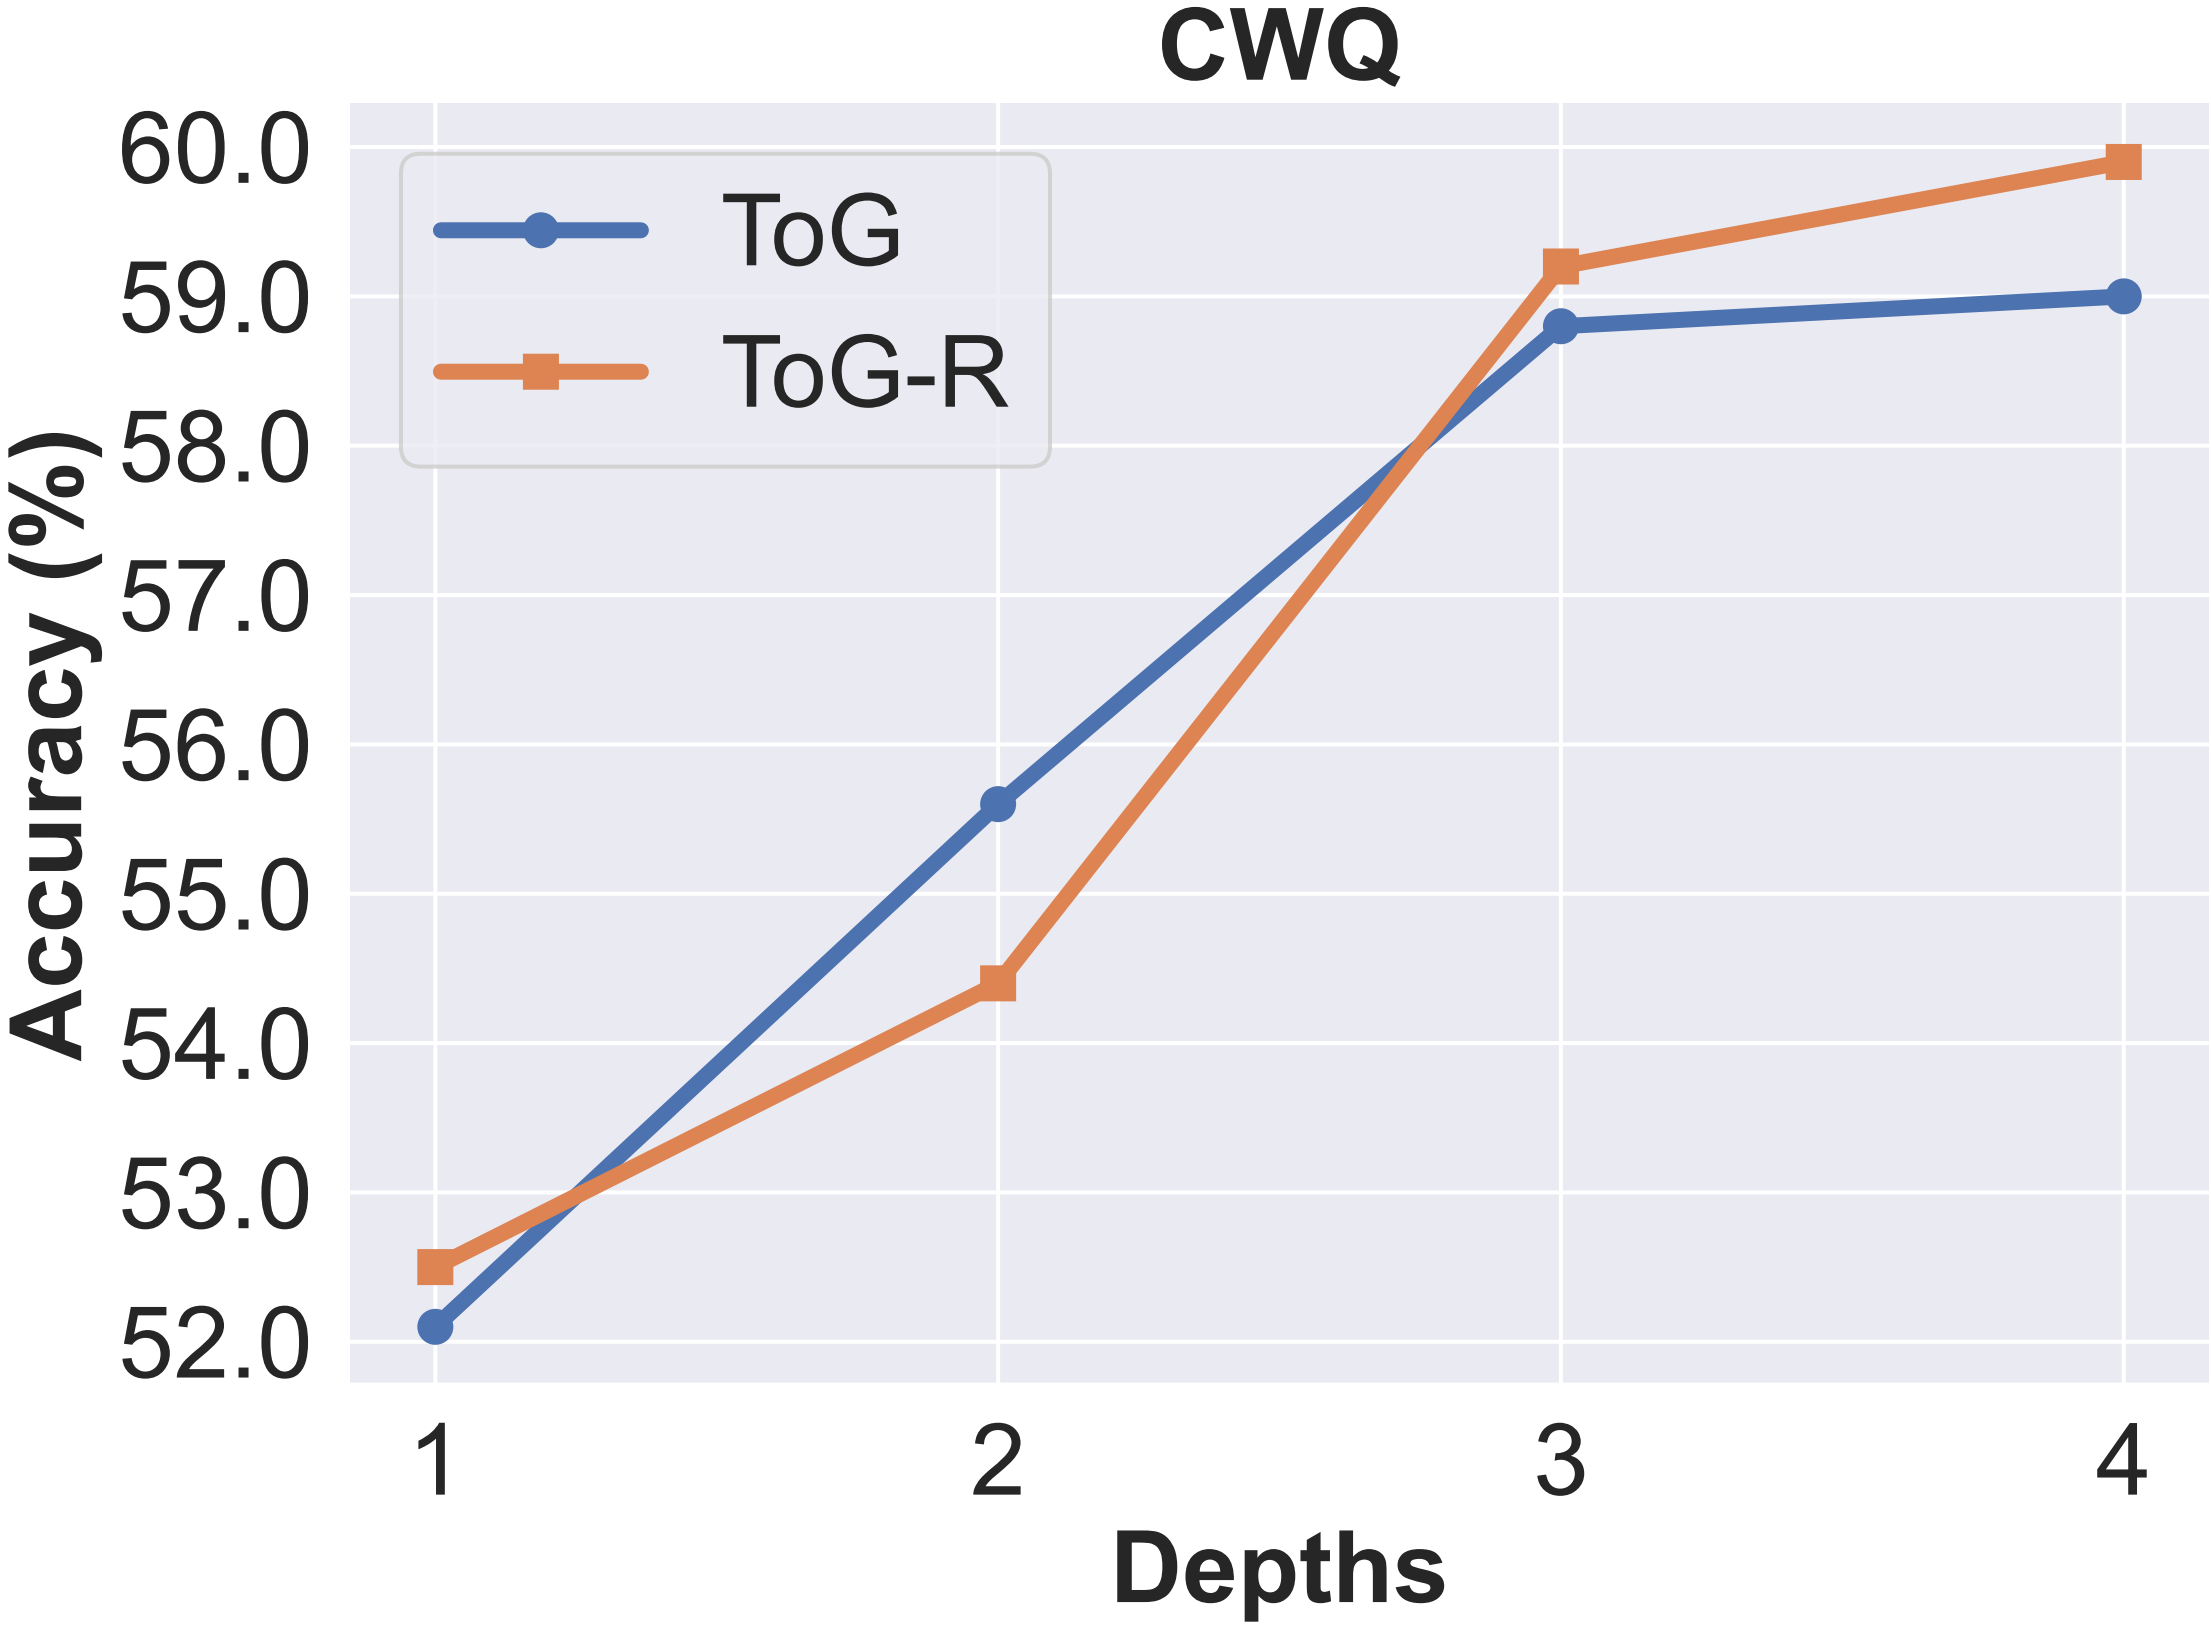
\includegraphics[width=\textwidth]{img/depth_cwq.png}
    \end{subfigure}
    \hfill
    \begin{subfigure}[b]{0.242\textwidth}
        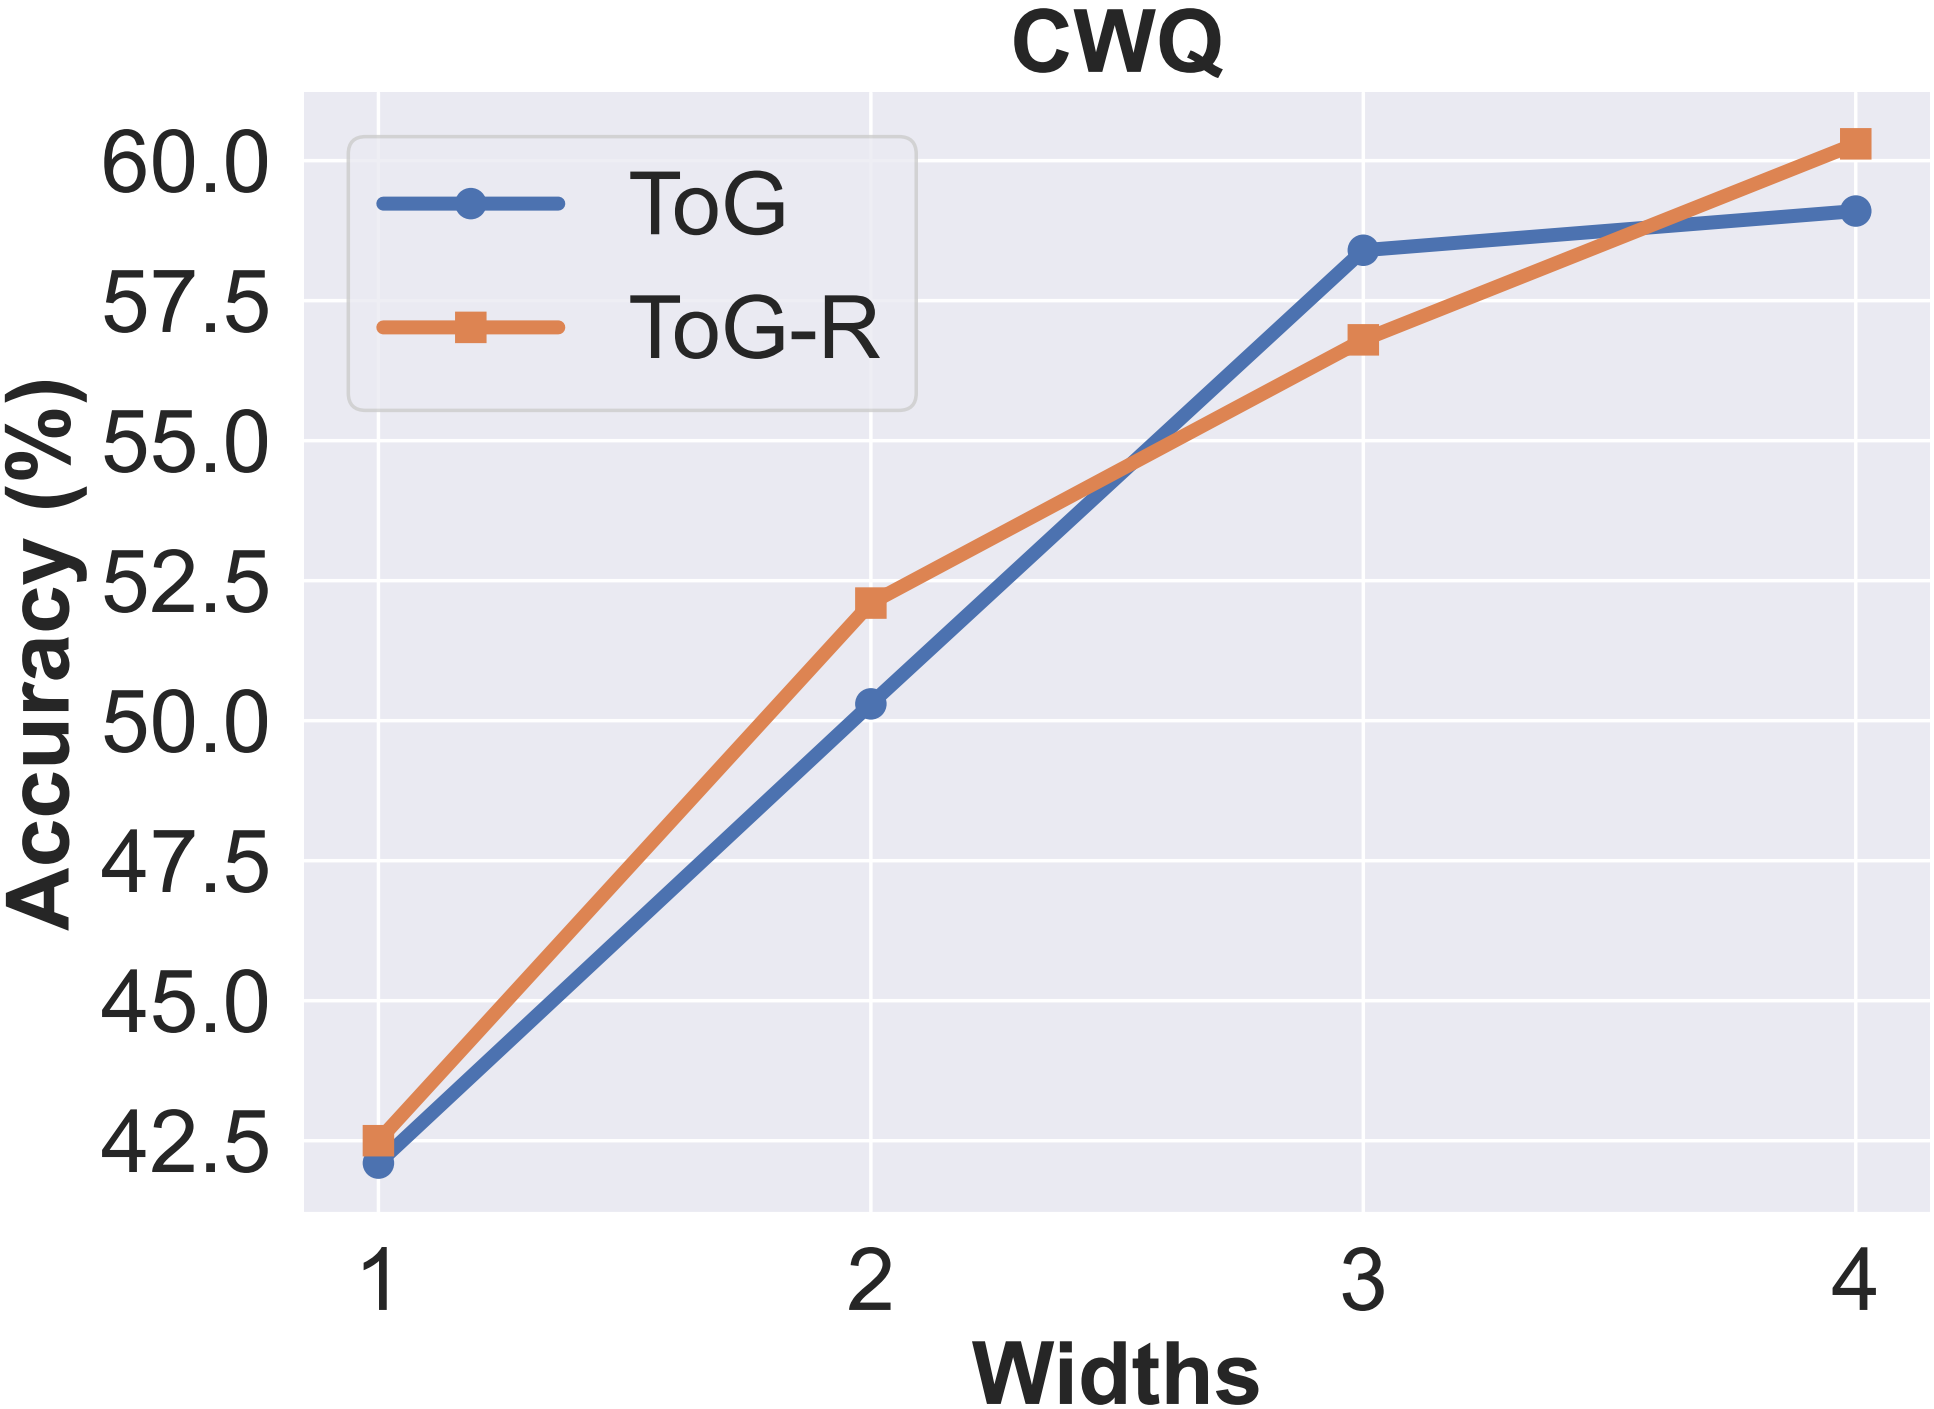
\includegraphics[width=\textwidth]{img/width_cwq.png}
    \end{subfigure}
    \hfill
    \begin{subfigure}[b]{0.242\textwidth}
        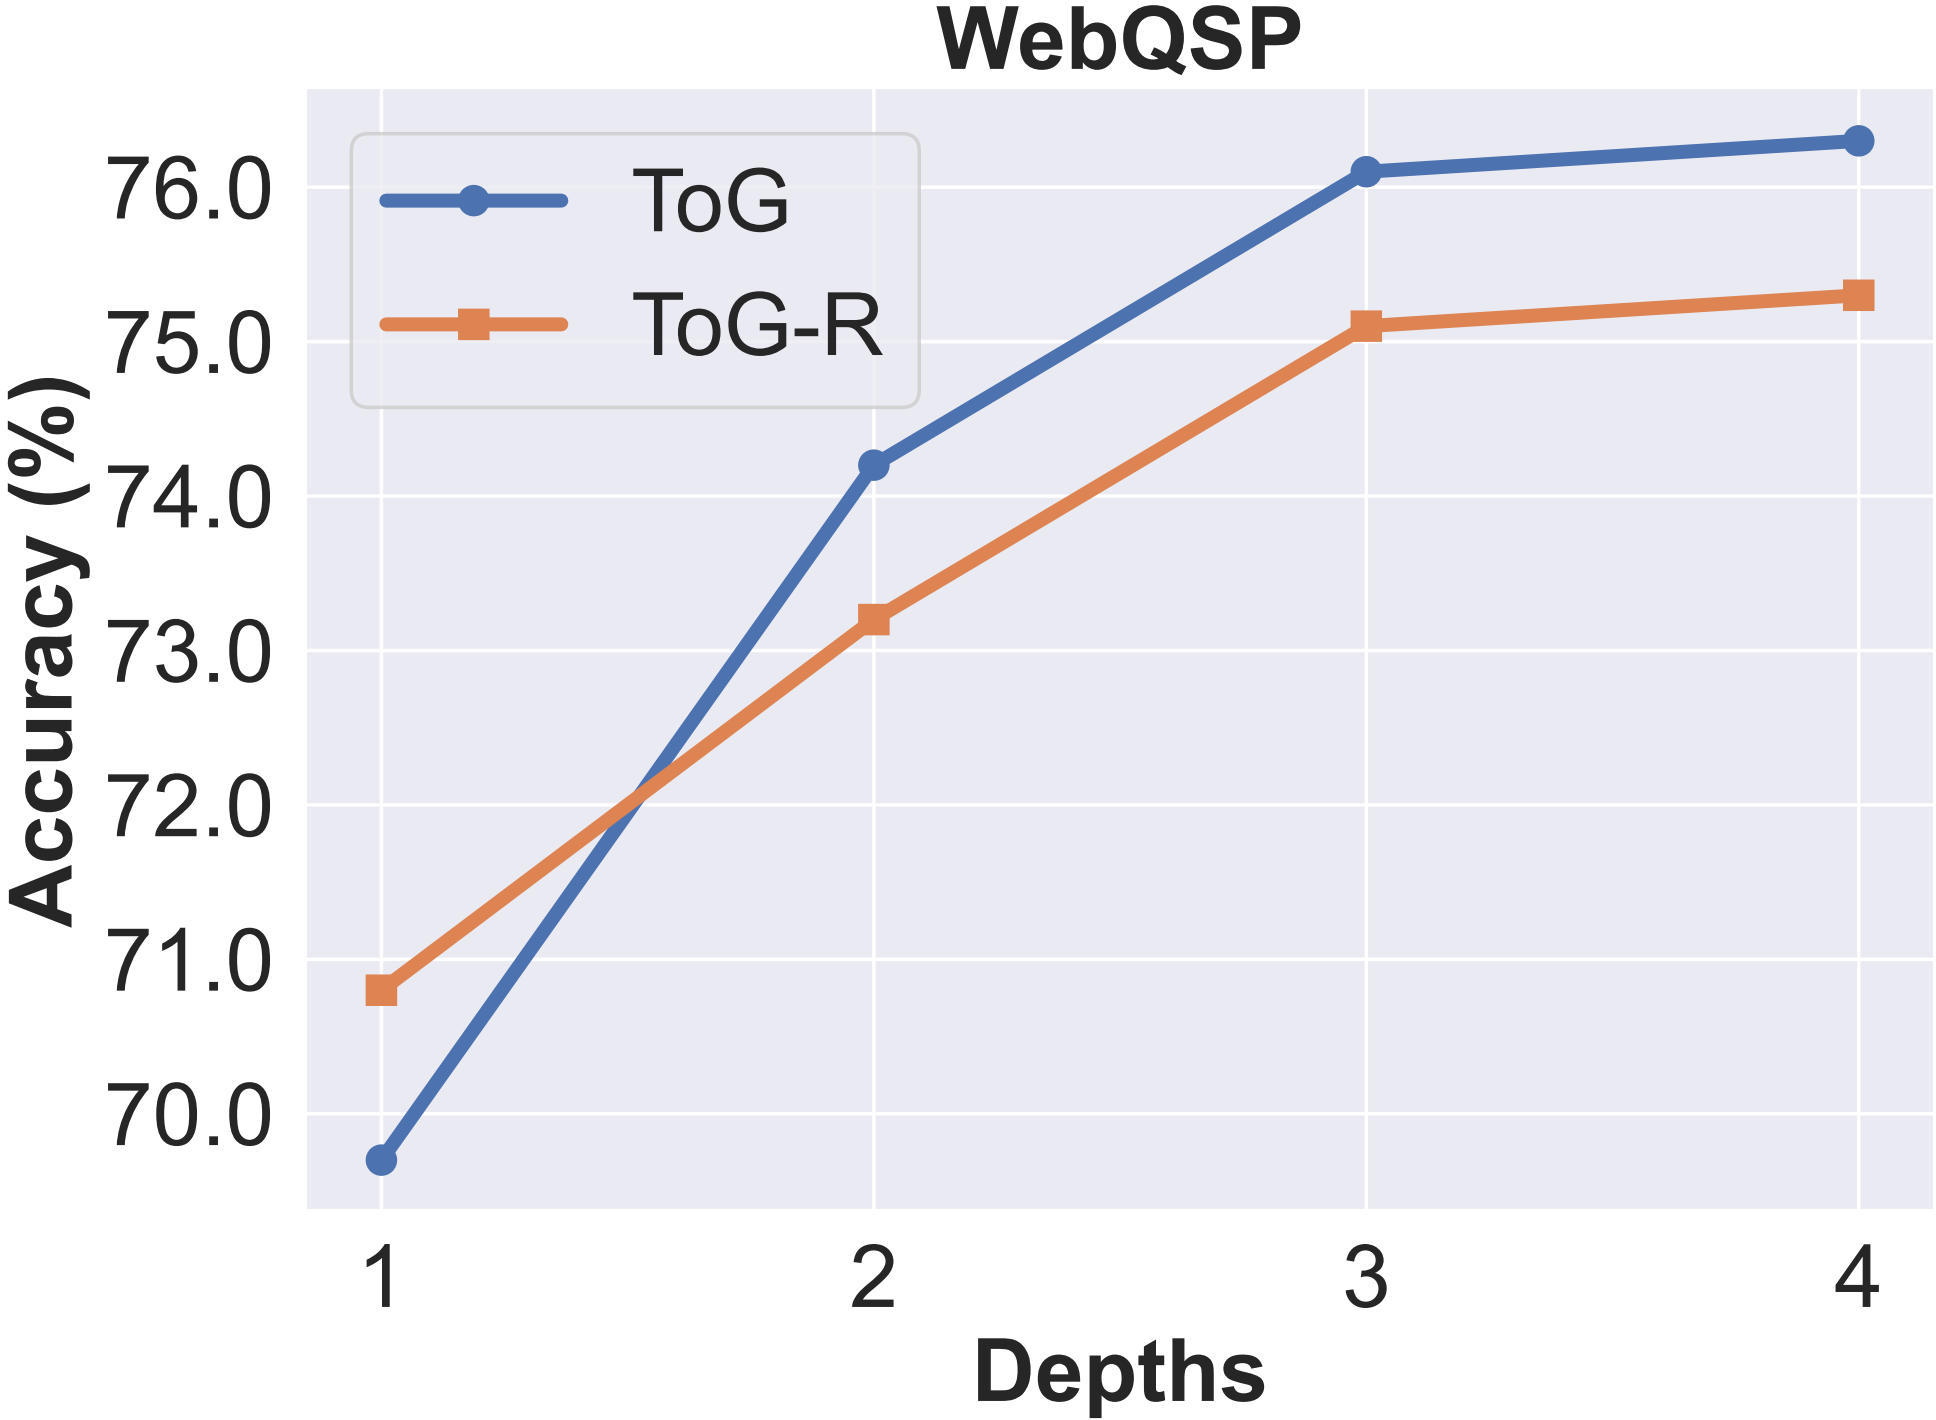
\includegraphics[width=\textwidth]{img/depth_webq.png}
    \end{subfigure}
    \hfill
    \begin{subfigure}[b]{0.242\textwidth}
        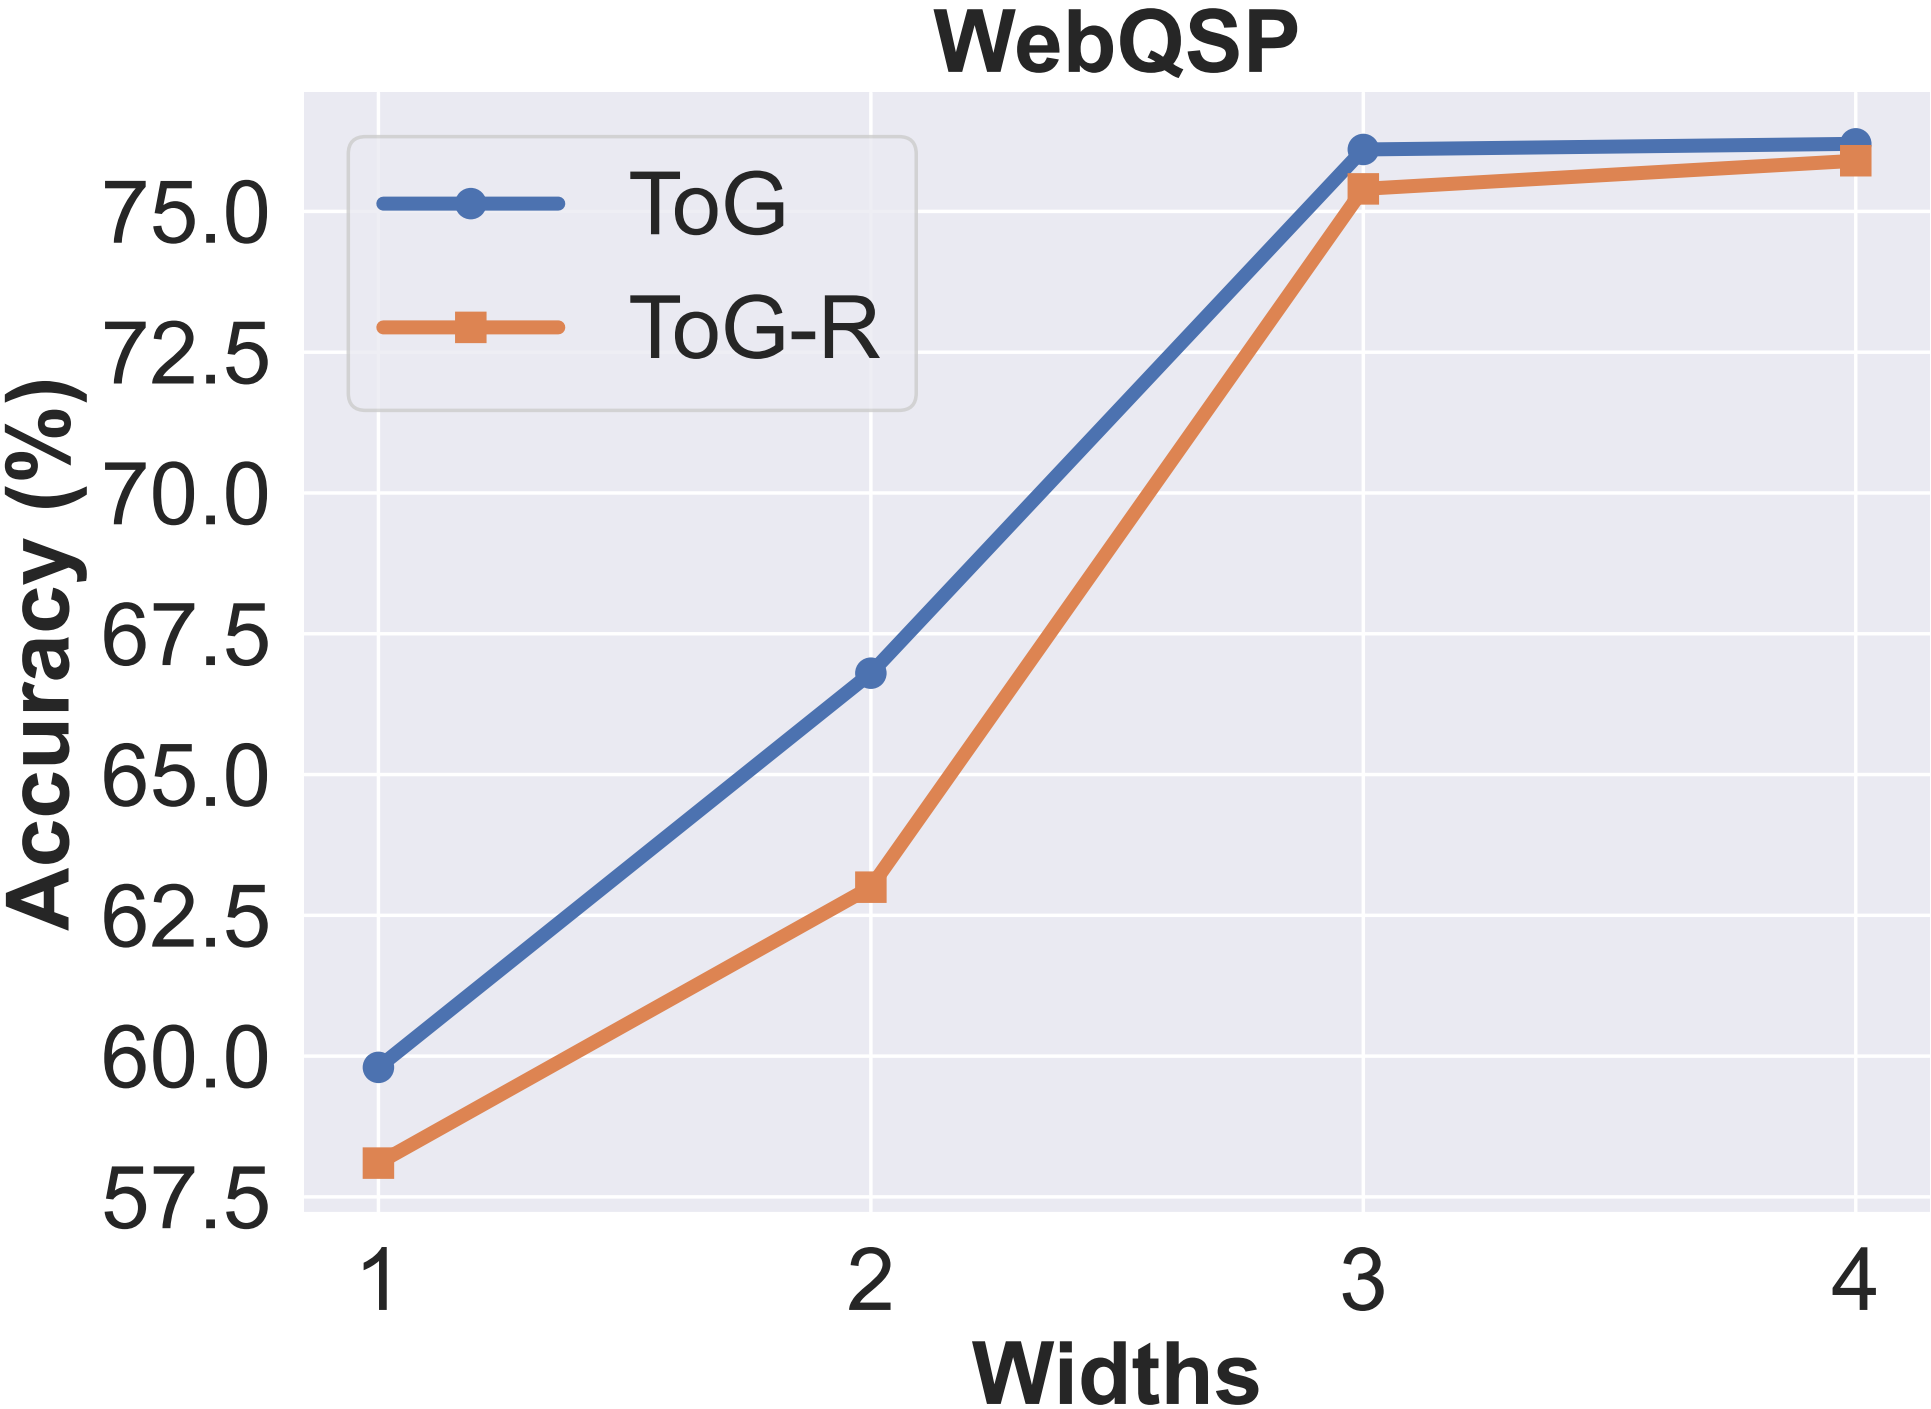
\includegraphics[width=\textwidth]{img/width_webq.png}
    \end{subfigure}
    \caption{Performances of ToG with different search depths and widths.}
    \label{fig: depth_width}
\end{figure}


\paragraph{Comparing the affects from different pruning tools.}
\label{sec: tools}

\begin{wraptable}{r}{0.4\textwidth}
\centering
\vspace{-0.5cm}
\resizebox{\linewidth}{!}{
\begin{tabular}{lcc}
\hline
\multirow{2}{*}{\textbf{Method}} & \multirow{2}{*}{\textbf{CWQ}} & \multirow{2}{*}{\textbf{WebQSP}} \\
                                 &                               &                              \\ \hline
\textbf{ToG}                   &                      &                      \\
w/BM25                           & 51.4                 & 58.7                 \\
w/SentenceBERT                   & 51.7                 & 66.3                 \\
w/ChatGPT                        & 58.8                 & 76.2                 \\ \hline
\textbf{ToG-R}                   & \multicolumn{1}{l}{} & \multicolumn{1}{l}{} \\
w/BM25                           & 49.4                 & 57.3                 \\
w/SentenceBERT                   & 50.1                 & 60.1                 \\
w/ChatGPT                        & 59.2                 & 75.1                 \\ \hline
\end{tabular}
}
\caption{Performances of ToG using different pruning tools.}
\label{table: tools}
\end{wraptable}
Other than the LLM, lightweight models that can measure text similarity like BM25 and SentenceBERT, can be employed as pruning tools in the exploration phase. We can select top-$N$ entities and relations based on their literal similarities with the question. We investigate the impacts of different pruning tools on the performance of the ToG, as demonstrated in Table \ref{table: tools}. The replacement of the LLM with either BM25 or SentenceBERT results in the significant performance degradation of our approach. Concretely, the results on CWQ drop on average by 8.4\%, and the results on WebQSP drop on average by 15.1\%.
The results show that the LLMs perform best as a pruning tool in terms of effectiveness. On the other hand, after utilizing
the BM25 or SentenceBERT, we only need $D + 1$ calls to the LLM instead of $2ND + D + 1$ as we
discuss in Section \ref{sec: reasoning}, which enhances the efficiency of ToG. 

We conduct additional ablation studies on the effect of the number of seed exemplars and the difference between ToG and naive beam search on the KG, which can be seen in Appendix~\ref{sec:ablation2}. 

\subsection{Knowledge Traceability and Correctability in ToG}
\label{sec: application}
The quality of KG is very important for correct reasoning by ToG. An interesting feature of ToG is knowledge traceability and knowledge correctability during LLM reasoning, and it provides a way to improve KG's quality using ToG itself and reduce the cost of KG construction and correction. As illustrated in Figure \ref{fig: app}, the explicit reasoning paths of the ToGs can be displayed to users. If potential errors or uncertainties in ToG answers are discovered by human users/experts or other LLMs, ToG has the ability to trace back and examine the reasoning path, find suspicious triples with errors, and correct them. 

%And upon a thorough self-evaluation conducted by either the LLM agent or a human expert, the causes of reasoning errors can be traced back to relevant incorrect triples in the KG, which can be rectified instantly. 

Take the case in Figure \ref{fig: app} as an example. Given the input question ``What is mascot Phillie Phanatic's team's spring training stadium?'', ToG outputs the wrong answer ``Bright House Field'' in the first round. Then ToG traces back all reasoning paths, localizes the cause of the error may come from the second reasoning path (Phillie Phanatic $\xrightarrow{\text{Team}}$ Philadelphia Phillies $\xrightarrow{\text{Arena Stadium}}$ Bright House Field), and analyzes that the error comes from the old name ``Specturm Field'' of ``Bright House Field'' in the outdated triple (\textit{Philadelphia Phillies}, \textit{Arena Stadium}, \textit{Bright House Field}). According to the hints from ToG, user can ask LLM to correct this error and answer the same question with correct information. This example reveals that ToG not only enhances LLM with KG, but also improves the quality of KG with LLM, known as knowledge infusion \citep{knowledge_infusion}. 
% ``\textit{Phillie Phanatic} $\to$ \textit{Team} $\to$ \textit{Philadelphia Phillies} $\to$ \textit{Arena Stadium} $\to$ \textit{Bright House Field}''

\begin{figure}[t]
	\centering
	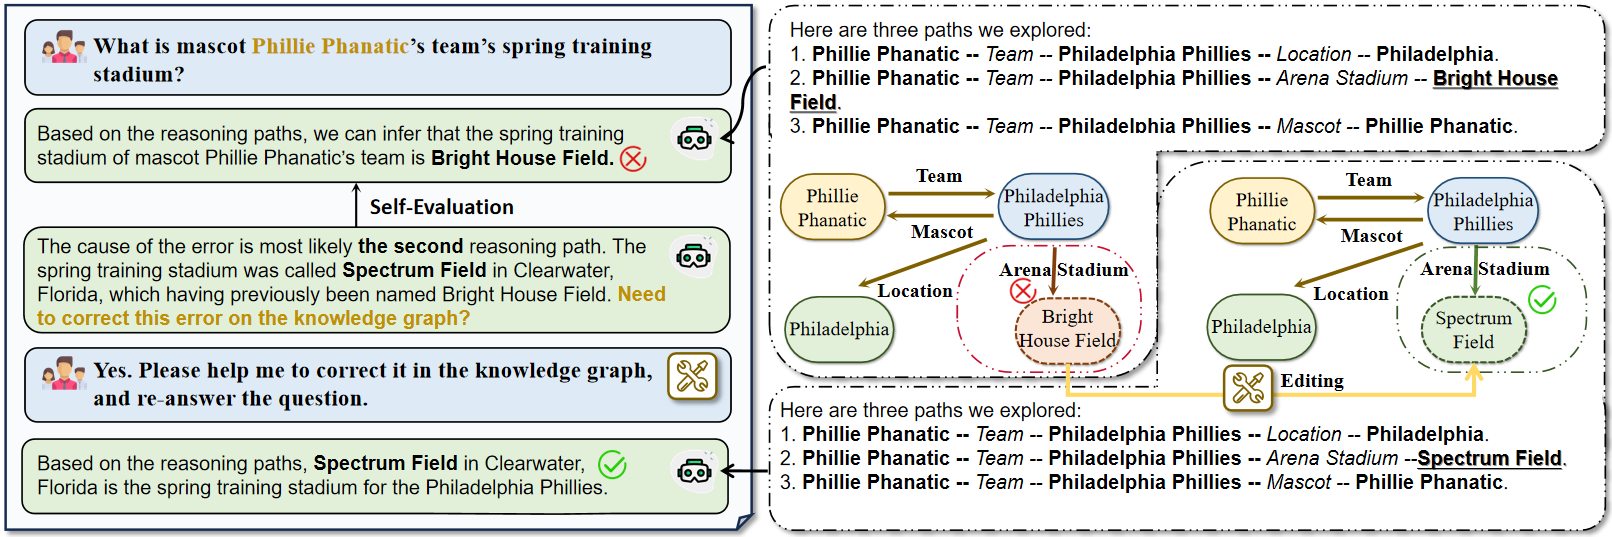
\includegraphics[width=0.99\columnwidth]{img/app.png}
	\caption{The illustration of knowledge traceability and correctability of ToG.}
         % \vspace{-10pt}
	\label{fig: app}
\end{figure}
% This specific path leverages the entity 'Philadelphia Phillies' and the relation 'Arena Stadium' to establish a connection, ultimately leading to the incorrect destination of 'Bright House Field'.



\section{Related Work}
% \paragraph{Knowledge Based Question Answering}
% In the field of knowledge-based question answering (KBQA), the goal is to find answers to questions by leveraging a structured knowledge base, such as Freebase \citep{freebase},wikidata \citep{10.1145/2629489}. Early approaches in KBQA can be broadly categorized into two main strategies: semantic parsing (SP) and information retrieval (IR).

% SP-based methods (\citep{berant2014semantic}, \citep{sun2020sparqa},\citep{mo2022transparent}) involve encoding the question and transforming it into an uninstantiated and syntactic logic form. These methods focus on understanding the underlying semantics of the question by mapping it to a logical representation. This allows for more structured reasoning and inference to be performed on the knowledge base to retrieve the relevant answer.

% On the other hand, IR-based methods (\citep{yang2016combining}, \citep{zhang2022subgraph}) aim to rank and retrieve topic entity-related subgraphs from the knowledge base. These subgraphs are then encoded, along with the question, using embedding tools such as BERT (\citep{liu2019bb}). The encoded representations are used to perform graph-based reasoning, enabling the system to locate and rank the most suitable candidate answer within the retrieved subgraphs.
% However, despite these achievements, there are still challenges that need to be addressed in KBQA. For instance, effectively handling complex questions with multiple facets, dealing with incomplete or noisy knowledge bases, and incorporating contextual information are areas that require further exploration and improvement.Our work was shown to find the correct chain of reasoning for the answer on an incomplete knowledge base rather retieving a big subgraph.
% \paragraph{}

\paragraph{Reasoning with LLM Prompting}
Chain-of-Thought (CoT) \citep{COT} has been shown to be effective in enhancing LLM reasoning. It creates a series of prompt instances according to reasoning logic under a few-shot learning paradigm in order to improve LLM's performance on complex tasks. The thought of CoT has been improved along different dimensions, including Auto-CoT \citep{auto}, Complex-CoT \citep{complex_cot}, Self-Consistency \citep{self_consistency}, Zero-Shot-CoT \citep{zero_shot_cot}, Iter-CoT \citep{iter-cot}, ToT \citep{tot}, GoT \citep{got} and so on. Given the limitation that all these works only use the knowledge in training data, recent efforts such as ReAct~\citep{yao2022react} attempt to utilize the information from external sources such as Wiki documents to further improve the reasoning performance. 

%Among different types of external knowledge sources, KGs are favored due to their dynamic, explicit, and structured knowledge representation~\citep{pan2023unifying}. In this work, we specifically focus on employing KGs as knowledge sources to enhance LLM's reasoning ability.

%In our research, we specifically focus on link inference within a knowledge graph. By retrieving a set of candidate entities and relations, we employ CoT as input to the LLM. The model then evaluates whether the links formed by these entities and relations are sufficient to infer the answer. While \citet{knowledgeaugmented} proposed a similar approach called Knowledge-Augmented Language Model Prompting, there are key distinctions in our methodology. Our approach utilizes a different set of links and candidates as CoT, whereas their approach directly samples the subgraph associated with the topic entity as the prompt for answer generation. Our emphasis lies more on the inference process rather than solely extracting the answer.

%By focusing on link inference, our research contributes to the advancement of knowledge-base question answering (KBQA) systems by leveraging CoT-based approaches. This enables the model to reason over the knowledge graph and evaluate the sufficiency of inferred links for answering the question at hand. The incorporation of CoT enhances the model's ability to handle complex reasoning tasks, leading to improved performance in terms of inference and answer quality.


\paragraph{KG-enhanced LLM} KG has advantages in dynamic, explicit, and structured knowledge representation~\citep{pan2023unifying} and techniques combining LLMs with KGs have been studied. Early studies~\citep{Knowbert,huang2024joint, luo2024rog, zhang2021poolingformer, li2023trea, liu2020reasoning} embed structured knowledge from KGs into the underlying neural networks during the pretraining or fine-tuning process. However, KG embedded in LLM sacrifices its own nature of explainability in knowledge reasoning and efficiency in knowledge updating~\citep{KELLMsurvey}.

Recent works instead combine LLMs with KGs by translating relevant structured knowledge from KGs to textual prompts for LLMs. All the methods follow a fixed pipeline that retrieves extra information from KGs to augment the LLM prompt and they belong to the $\hbox{LLM}\oplus \hbox{KG}$ paradigm we defined in the introduction section. On the other hand, \citet{structgpt} asks LLM to explore KG and so it can be regarded as a special case of ToG, which belongs to the $\hbox{LLM}\otimes \hbox{KG}$ paradigms. 

% For example, \citet{DB-BLINDER} generates the backbone of SPARQL queries using the LLM and fills them with complete information using KGs. \citet{knowledgeaugmented} samples the triples containing the entities appearing in question for LLM inference.

% \paragraph{Knowledge Intensive NLP Task}
% The use of external knowledge or textual resources has gained significant attention in recent papers aiming to address the knowledge limitations of LLMs. There are two main approaches to making a LLM more knowledgeable: incorporating an external knowledge base for question answering or directly utilizing the knowledge base during pre-training or fine-tuning. For instance, RAG (Retrieval-Augmented Generation) (\citep{lewis2021retrievalaugmented}) employs a retriever to rank and extract relevant documents, which are then used as input to a generator for generating the final answer. Another notable example is ERNIE (Enhanced Representation through kNowledge IntEgration), proposed by \citet{zhang2019ernie}. ERNIE utilizes informative entities from knowledge graphs (KGs) for pre-training and exhibits strong performance in various knowledge-driven tasks. Recently there have been many approaches to explore LLM knowledge enhancement around ChatGPT.\citet{cok} uses LLM to split the question and uses generator to generate different spraql to retrieve the answer and let the LLM generate the answer itself. In our approach, we leverage external knowledge as a prompt. However, instead of simply retrieving a portion of the information, we assign the task of retrieving and evaluating different relations and entity scores directly to the LLM. The model then selects the appropriate number of relations during this process. By repeating this procedure, we obtain an inference path rather than a set of documents containing redundant information. By adopting this approach, our research extends the existing methods of incorporating external knowledge. We empower the LLM to actively retrieve and evaluate relevant relations and entities, allowing for more focused and selective reasoning. This enables the model to construct an inference path tailored to the specific question, enhancing its ability to generate accurate and meaningful answers.


\section{Conclusion}
We introduce the $\hbox{LLM}\otimes \hbox{KG}$ paradigm for integrating LLMs and KGs in a tight-coupling manner, and propose the Think-on-Graph (ToG) algorithmic framework which leverages LLM as a agent participating in KG reasoning for better decision-making. Experimental results demonstrate that ToG outperforms existing fine-tuning-based methods and prompting-based methods without additional training cost and mitigates the hallucination issue of LLMs.

\section{Acknowledgement}
We express our sincere gratitude to the esteemed reviewers for their invaluable feedback and constructive comments, which significantly contributed to the improvement and refinement of this paper. Their insightful suggestions and meticulous attention to detail have played a pivotal role in enhancing the quality and clarity of our research work.

\bibliography{iclr2024_conference}
\bibliographystyle{iclr2024_conference}

%%%%%%%%%%%%%%%%%%%%%%%%%%%%%%%%%%%%%%%%%%%%%%%%%%%%%%%%%%%%

\newpage

\appendix

\section{Algorithm for ToG}
We summarize the comprehensive algorithmic procedure of ToG and ToG-R, as shown in Figure Algorithm \ref{algorithm1} and \ref{algorithm2}.

\begin{figure}[htb]
\begin{minipage}[t]{0.5\textwidth}
\begin{algorithm}[H]
\begin{algorithmic}
\Require Input $x$, LLM $\pi$, depth limit $D_{max}$ sample limit $N$.
\State Initialize $E^{0} \gets $ Extract entities on $x$, $P \gets []$, $M \gets 0$.
\While {$D$ $\leq$ $D_{max}$} 
    \State  $R^{D}_{cand}$, $P_{cand}$  $ \gets $ Search($x$, $E^{D-1}$, $P$)
    \State $R^{D}$, $P$  $\gets $ Prune($\pi$, $x$,  $R^{D}_{cand}$, $P_{cand}$) 
    \State $E^{D}_{cand}$, $P_{cand}$  $\gets $ Search($x$, $E^{D-1}$, $R^{D}$, $P$)
    \State $E^{D}$, $P$ $\gets $ Prune($\pi$, $x$,  $E^{D}_{cand}$, $P_{cand}$)
    % \State Update $P = P \cup \sum_{i=1}^{N}(e_s^{i}, r^{i}, e_o^{i})$
    \If {Reasoning($\pi$, $x$, $P$)} 
        \State Generate($\pi$, $x$, $P$)
        \State \textbf{break}
    \EndIf
    \State Increment $D$ by 1.
\EndWhile%
\If {$D$ $>$ $D_{max}$}
    \State Generate($\pi$, $x$)
\EndIf
\caption{ToG}
\label{algorithm1}
\end{algorithmic}
\end{algorithm}
\end{minipage}
\begin{minipage}[t]{0.5\textwidth}
\begin{algorithm}[H]
\begin{algorithmic}
\Require Input $x$, LLM $\pi$, depth limit $D_{max}$ sample limit $N$.
\State Initialize $E^{0} \gets $ Extract entities on $x$, $P \gets []$, $M \gets 0$.
\While {$D$ $\leq$ $D_{max}$} 
    \State  $R^{D}_{cand}$, $P_{cand}$  $ \gets $ Search($x$, $E^{D-1}$, $P$)
    \State $R^{D}$, $P$  $\gets $ Prune($\pi$, $x$, $R^{D}_{cand}$, $P_{cand}$) 
    \State $E^{D}_{cand}$, $P_{cand}$  $\gets $ Search($x$, $E^{D-1}$, $R^{D}$, $P$)
    % \State Update $P = P \cup \sum_{i=1}^{N}(e_s^{i}, r^{i}, e_o^{i})$
    \If {Reasoning($\pi$, $x$, $P$, $E^{D}_{cand}$)} 
        \State Generate($\pi$, $x$, $P$, $E^{D}_{cand}$)
        \State \textbf{break}
    \EndIf
    \State $E^{D}$, $P$ $\gets $ Random\_Prune($E^{D}_{cand}$, $P_{cand}$)
    \State Increment $D$ by 1.
\EndWhile%
\If {$D$ $>$ $D_{max}$}
    \State Generate($\pi$, $x$)
\EndIf
\caption{ToG-R}
\label{algorithm2}
\end{algorithmic}
\end{algorithm}
\end{minipage}
% \begin{minipage}[t]{0.5\textwidth}
% \begin{algorithm}[H]
% \begin{algorithmic}
% \Require Input $x$, LLM $p_\theta$, depth limit $D_{max}$, sample limit $N$.
% \State Initialize $E_{c} \gets $ Extract entities $x$, $P \gets []$, $depth \gets 0$.
% \While {depth $\leq$ $D_{max}$}
%     \State $R_{cand} \gets $ Search($x$, $E_{c}$)
%     \State $R_c  \gets $ Prune($x$, $R_{cand}$, $E_{c}$)
%     \State $E_{cand} \gets $ Entity\_Search($x$, P, $R_c$)
%     % \State $E_c \gets $ Prune($x$, $R_c$, $E_{cand}$)
%     \State Update $P = P \cup R_c$
%     \If {Reasoning($p_\theta$, $x$, P, $E_{cand}$)} 
%         \State Generate($p_\theta$, $x$, P)
%         \State \textbf{break}
%     \EndIf
%     \State Increment $depth$ by 1.
% \EndWhile
% \If {not Reasoning($p_\theta$, $x$, P, $E_{cand}$)}
%     \State Generate($p_\theta$, $x$)
% \EndIf
% \vspace{12.8pt}
% \caption{Relation-based ToG}
% \label{algorithm2}
% \end{algorithmic}
% \end{algorithm}
% \end{minipage}
\end{figure}


\section{Additional Ablation Study and Experiment Analysis}
In this section, we conduct more experiments for ablation study in addition to Section \ref{sec:ablation1}, and analyze experimental results of ToG in detail.

\subsection{Additional Ablation Study}~\label{sec:ablation2}
\paragraph{Sensitivity to the Number of Seed Examplars}
To better understand how sensitive ToG is sensitivity to the number of seed exemplars, we employ sensitivity analysis shown in Figure \ref{fig: shots}. We conduct zero-shot experiment and select 1-6 examples from the training set as few-shot setting. In the few-shot tests, we randomly chose $M$ of $\{1,2,3,4,6\}$ exemplars as demonstrations and replicated the experiments three times. As the number of examples in the demonstrations increases, the overall performance also generally improves. However, the performance peaks for ToG and ToG-R differ (with the best performance for ToG at 5-shot and for ToG-R at 4-shot). Moreover, ToG's zero-shot performance outpaces ToG-R. This can be attributed to ToG having fully completely explored paths, ensuring commendable performance even in zero-shot. In contrast, ToG-R omits entities in the path, but its average performance with demonstrations is superior to ToG.

\begin{figure}[t]
    \centering
    \begin{subfigure}[b]{0.49\textwidth}
        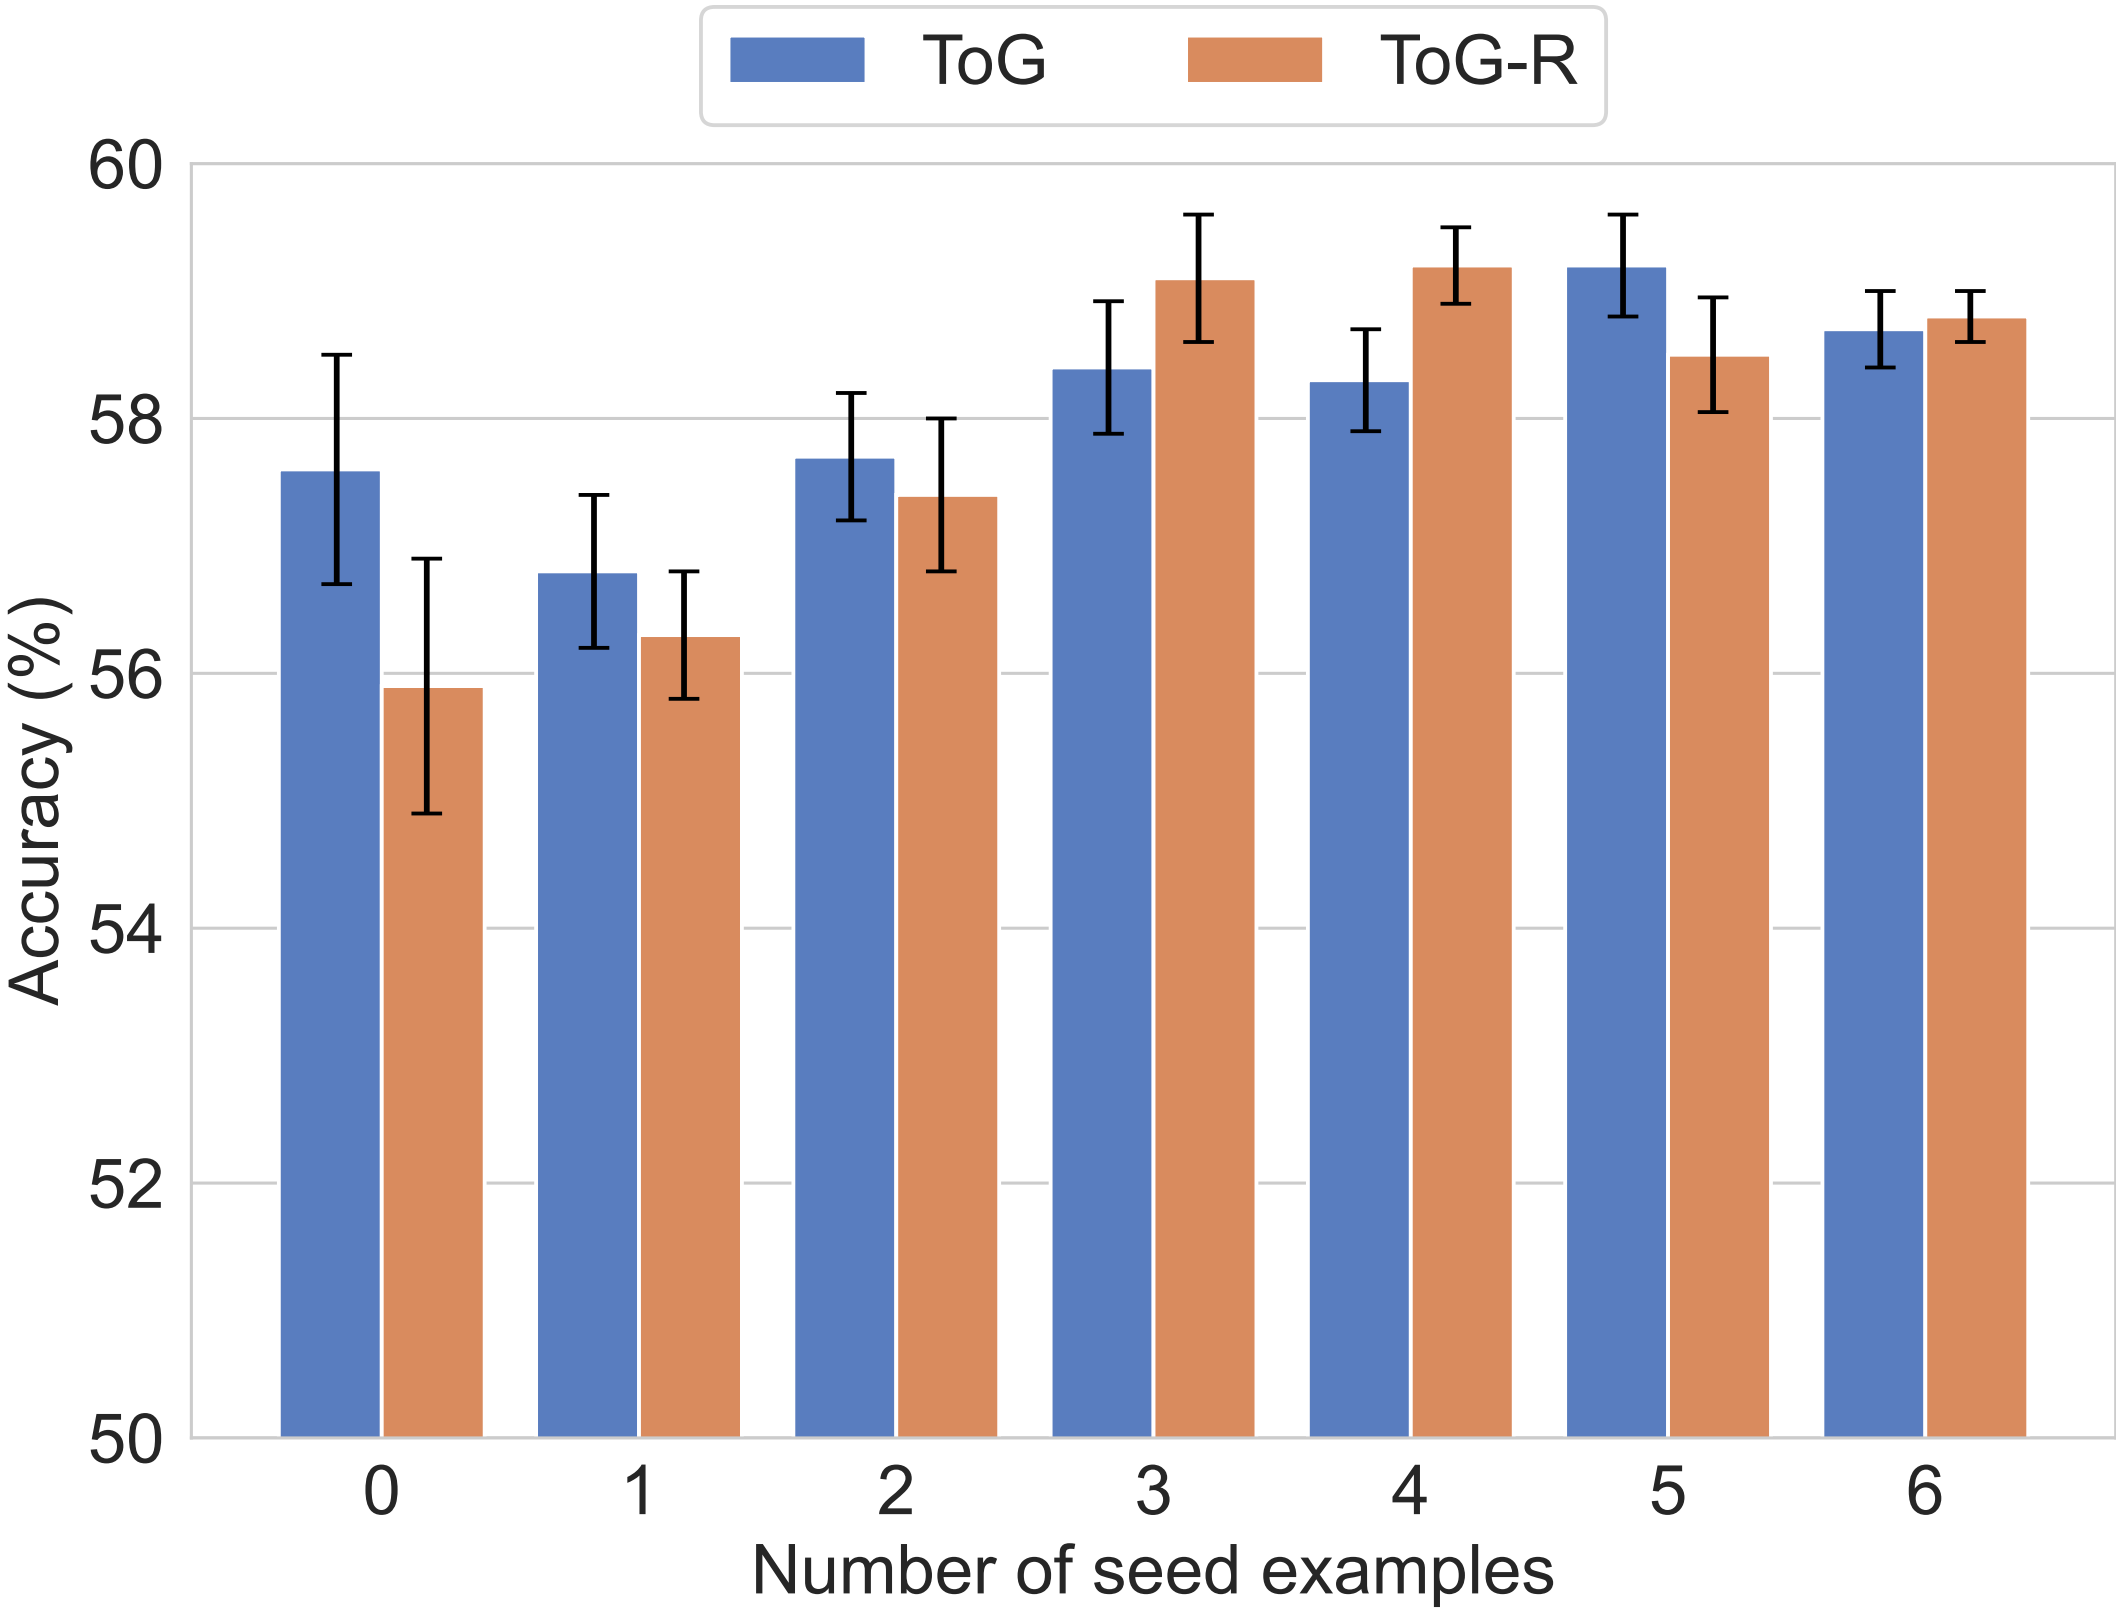
\includegraphics[width=\textwidth]{img/shot_cwq_with_error_bars.png}
    \end{subfigure}
    \hfill
    \begin{subfigure}[b]{0.49\textwidth}
        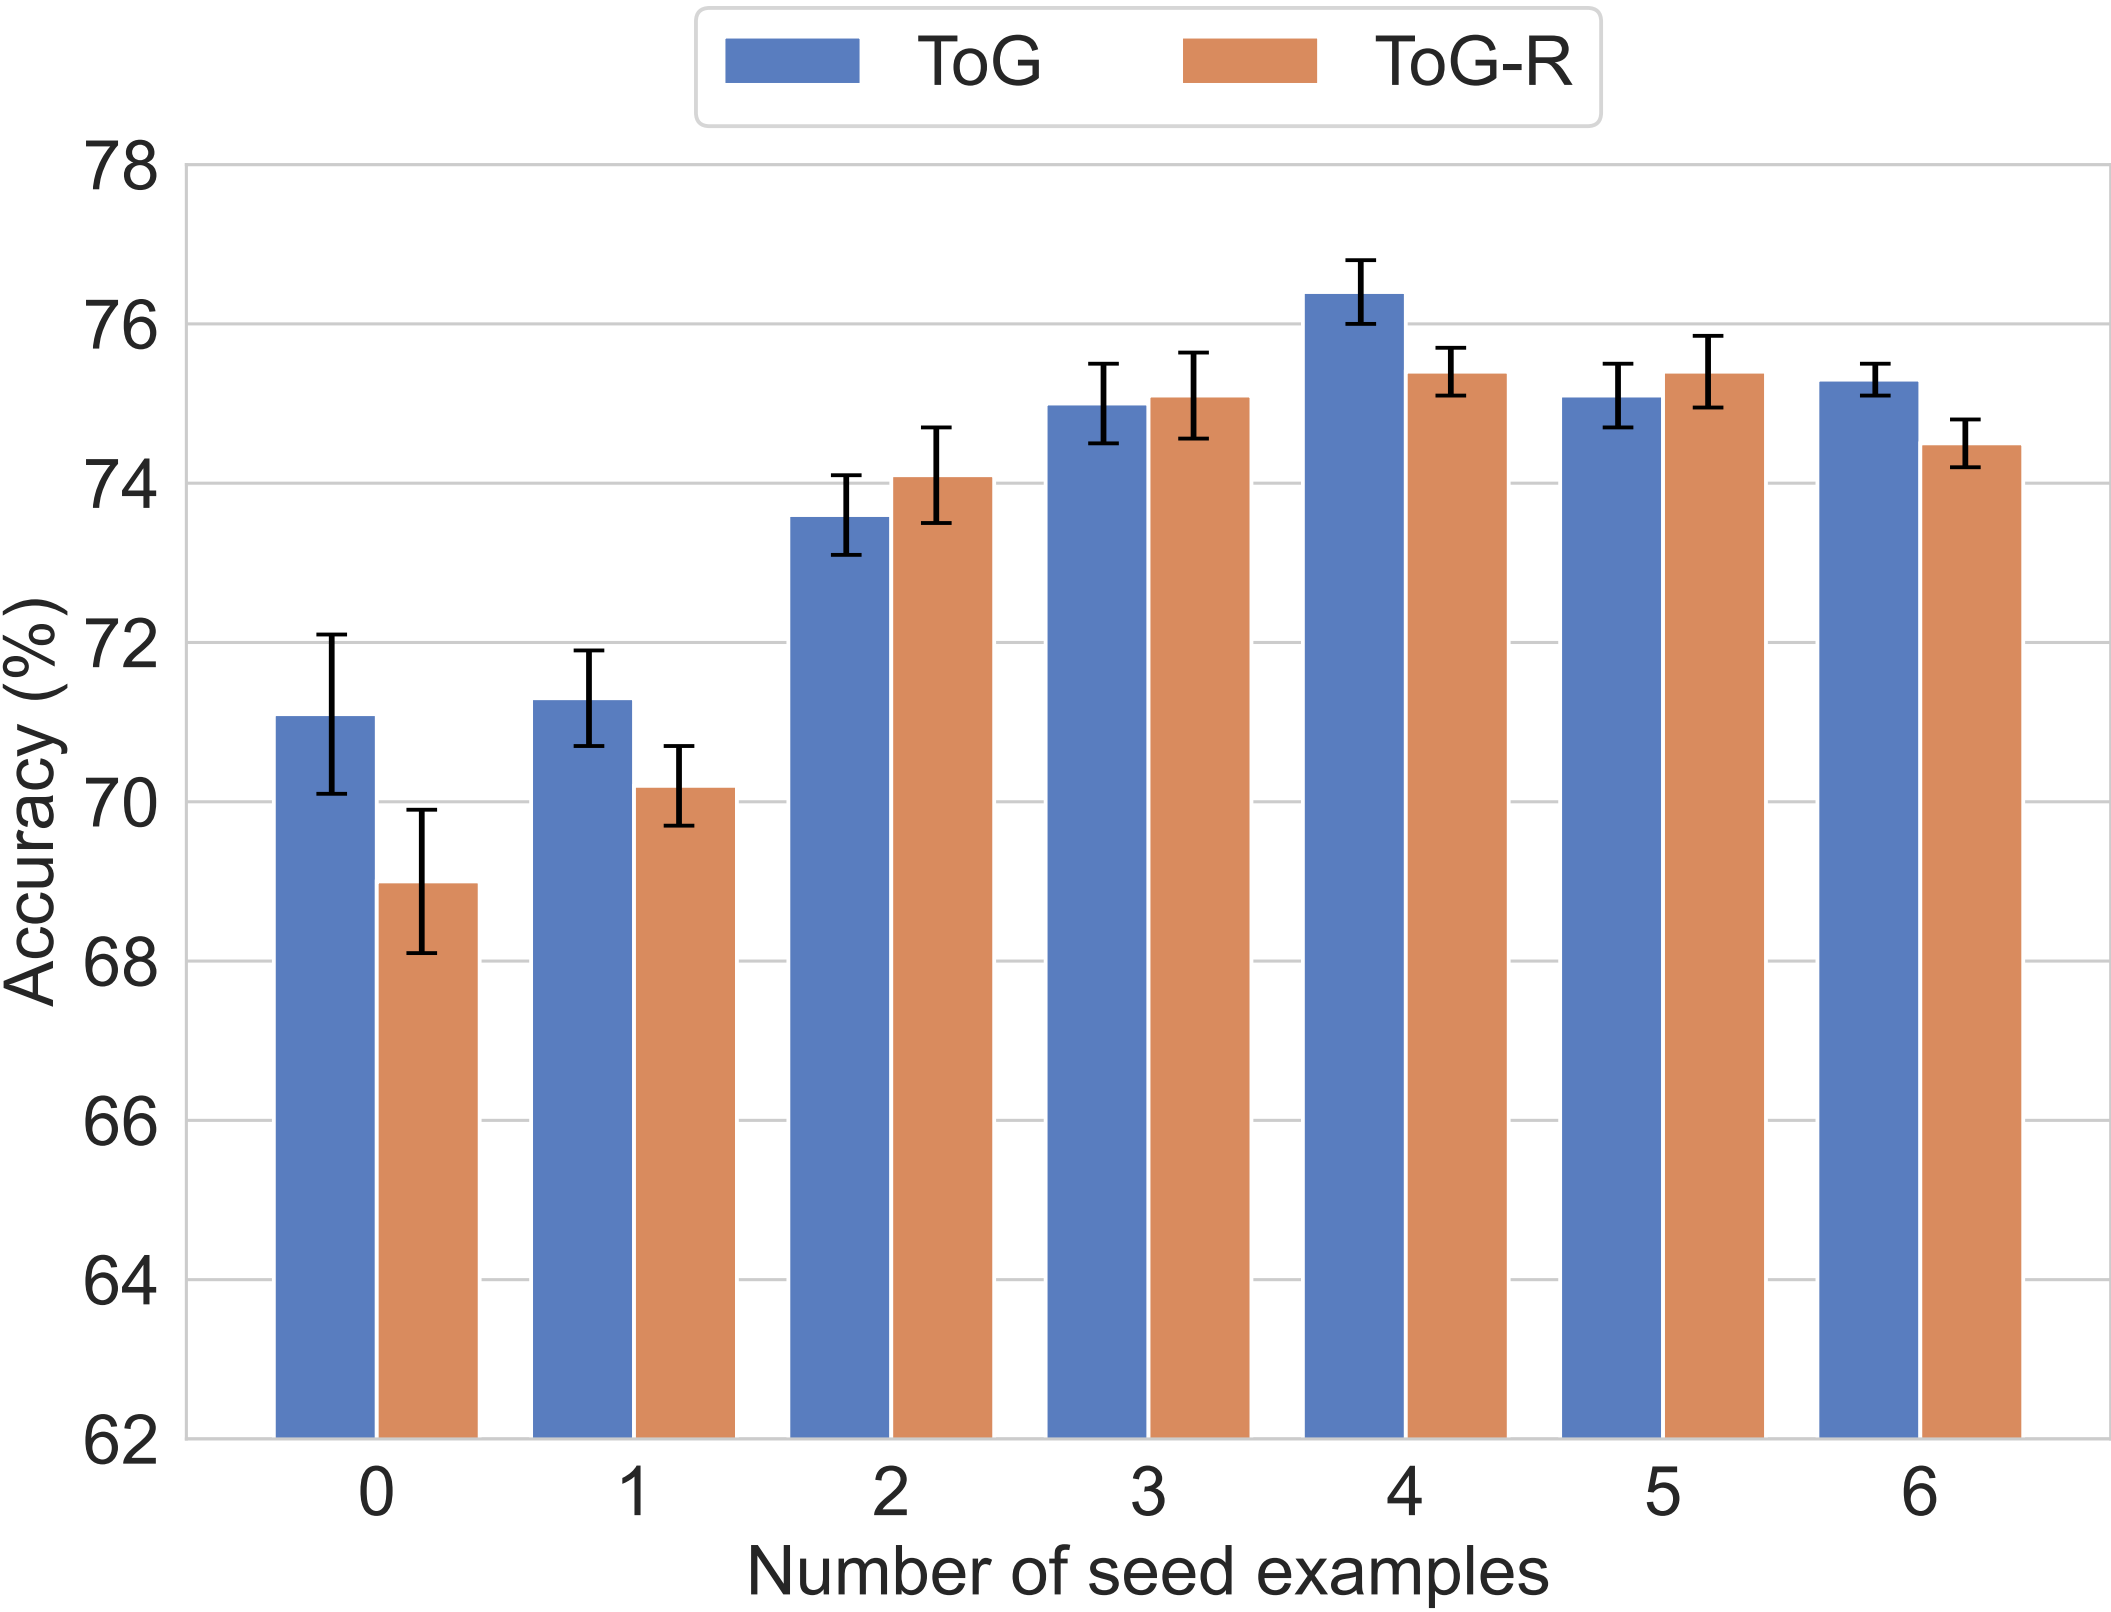
\includegraphics[width=\textwidth]{img/shot_webq_with_error_bars.png}
    \end{subfigure}
    \caption{Exemplar sensitivity analysis for CWQ and WebQSP for ToG, where "0" denotes zero-shot and "k" denotes k-shot.}
    \label{fig: shots}
\end{figure}

\begin{figure}[t]
    \centering
    \begin{subfigure}[b]{0.32\textwidth}
        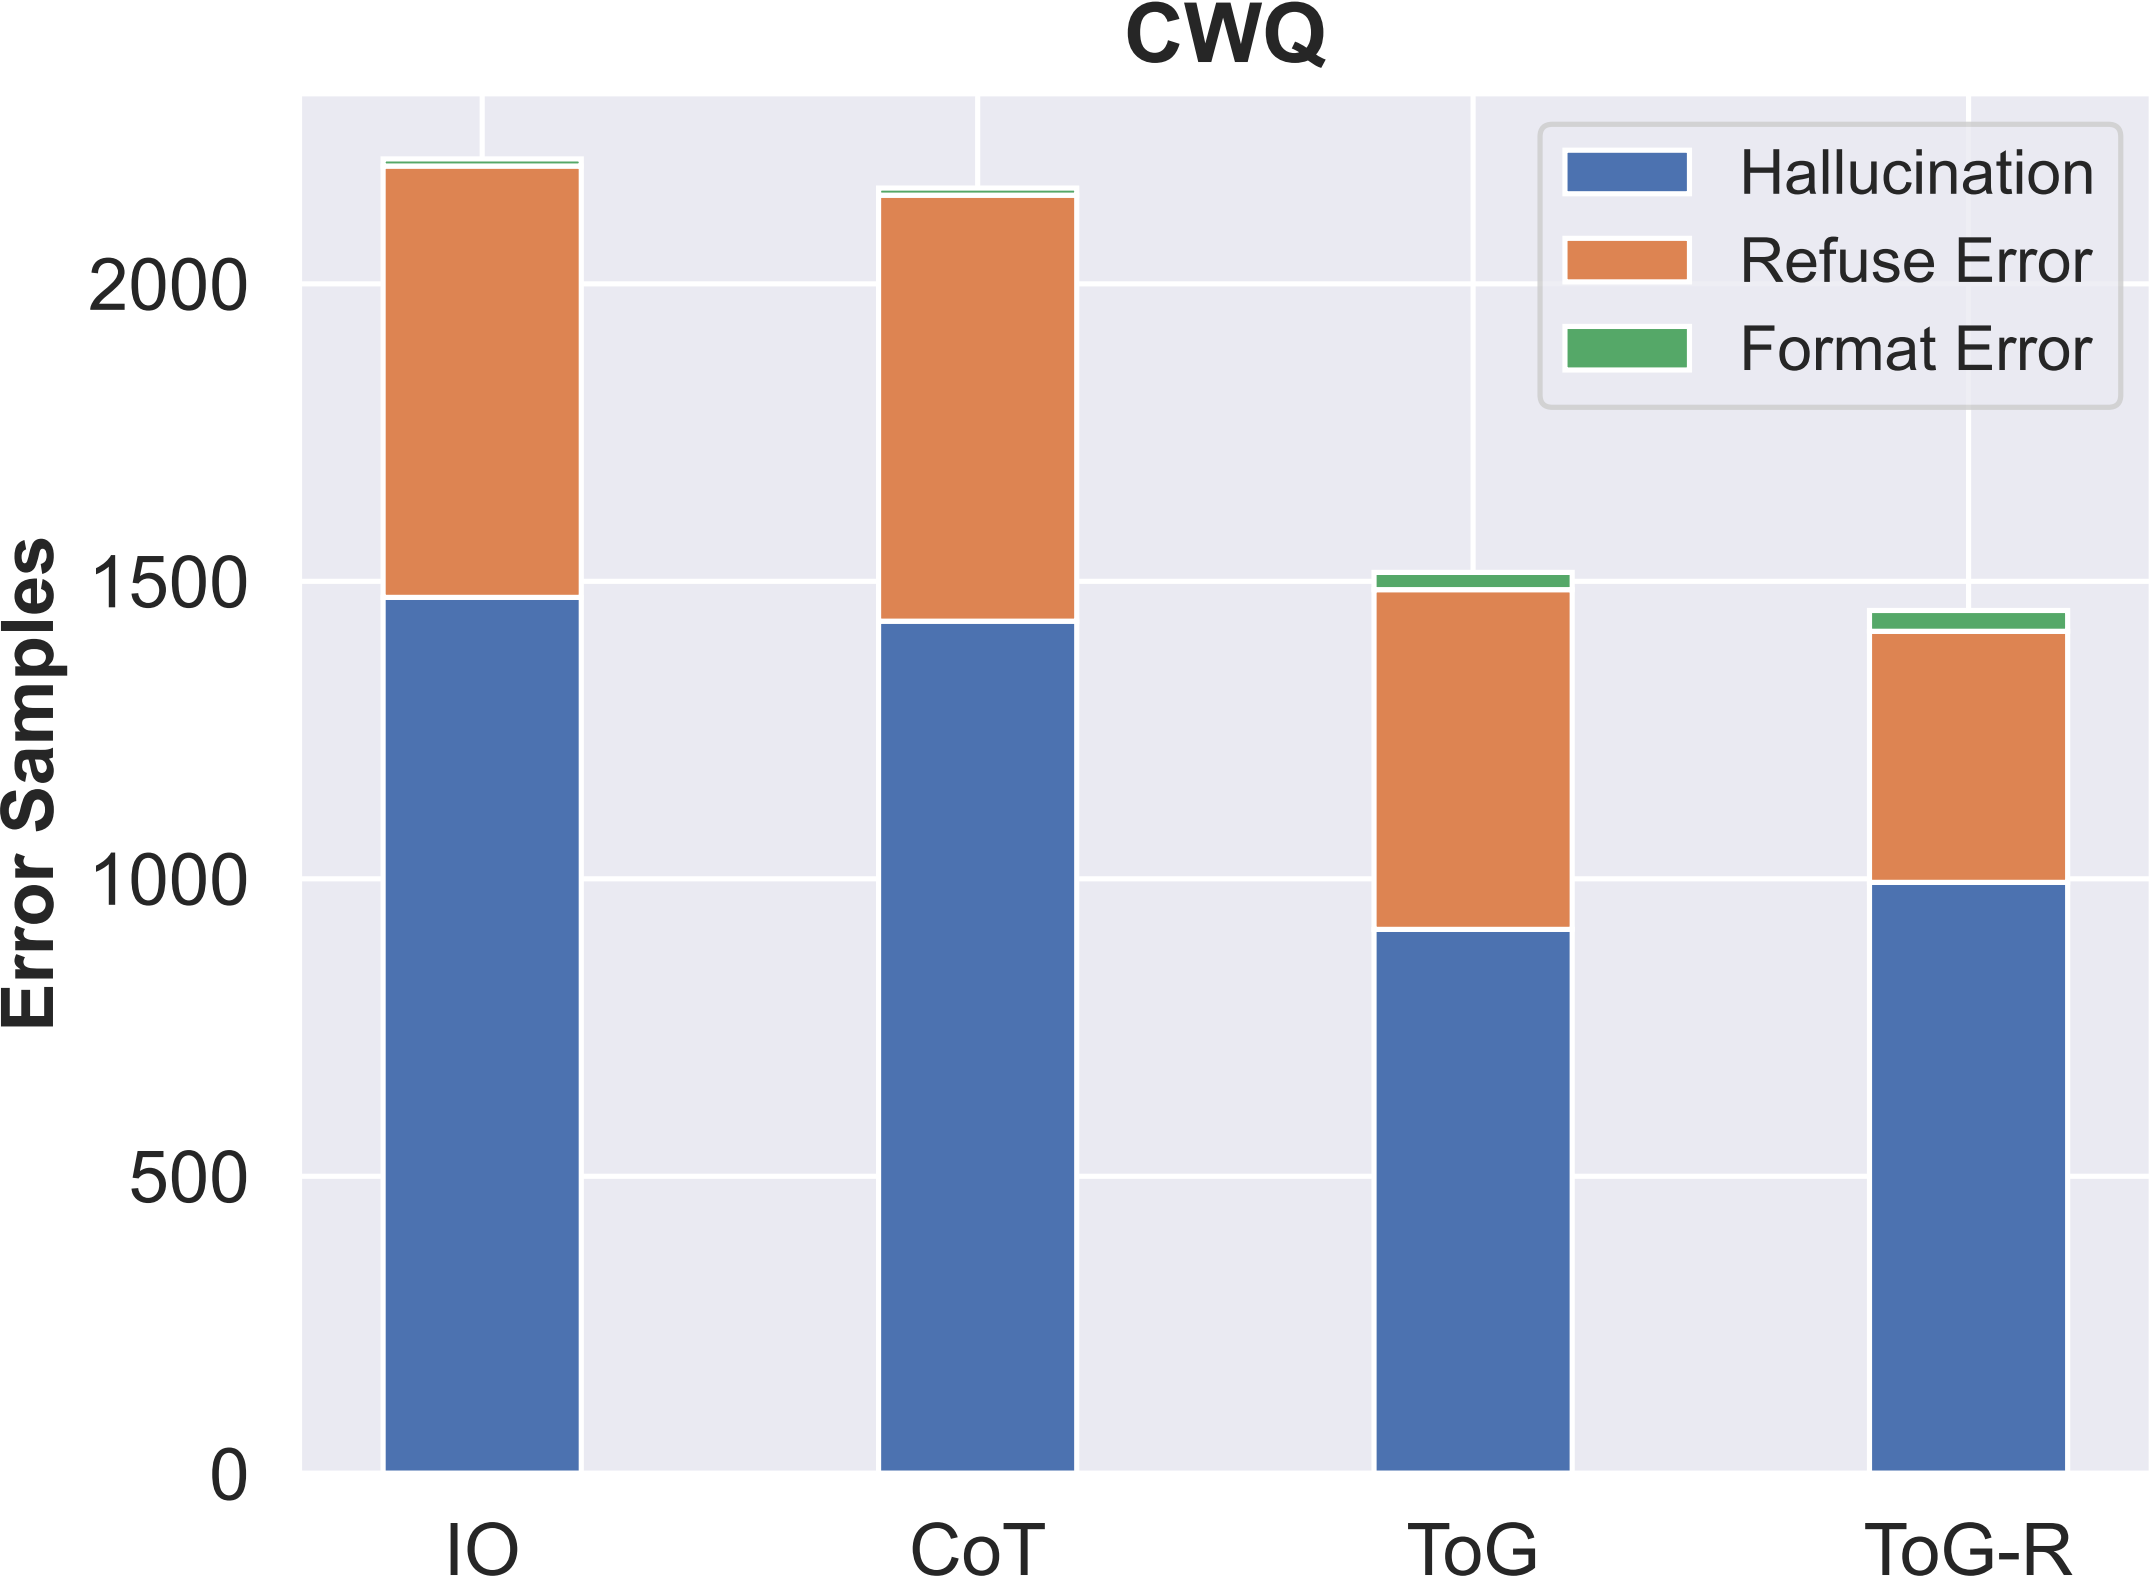
\includegraphics[width=\textwidth]{img/error_bar_cwq.png}
    \end{subfigure}
    \hfill
    \begin{subfigure}[b]{0.32\textwidth}
        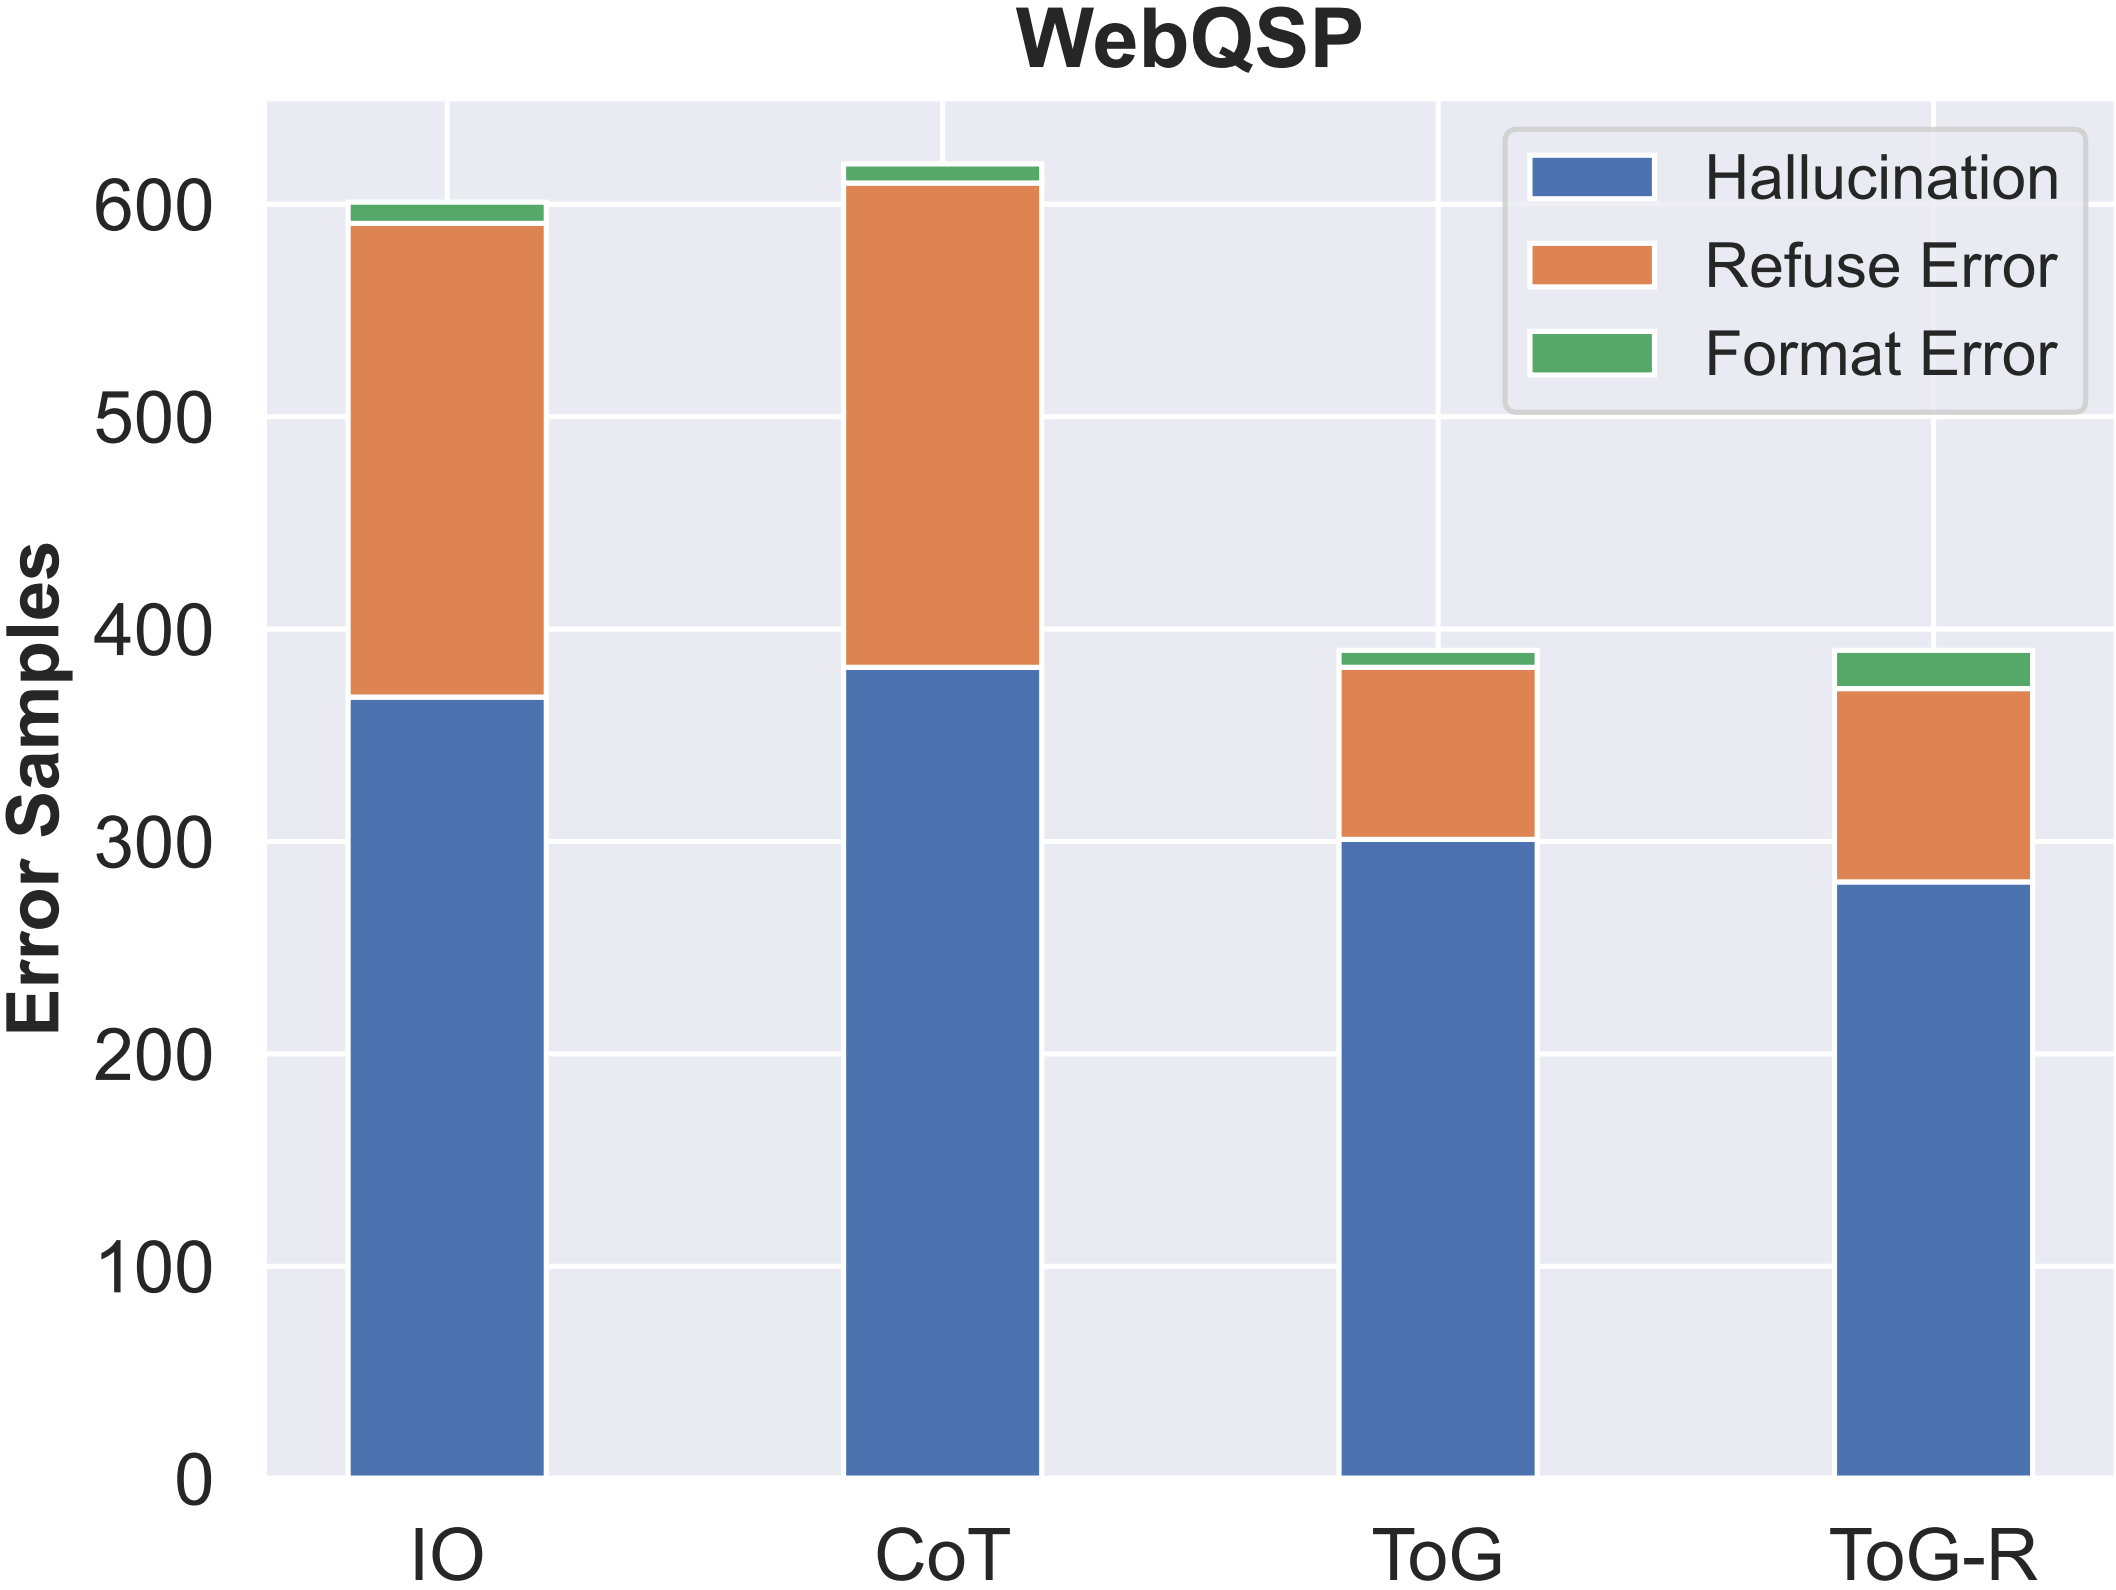
\includegraphics[width=\textwidth]{img/error_bar_webqsp.png}
    \end{subfigure}
    \hfill
    \begin{subfigure}[b]{0.32\textwidth}
        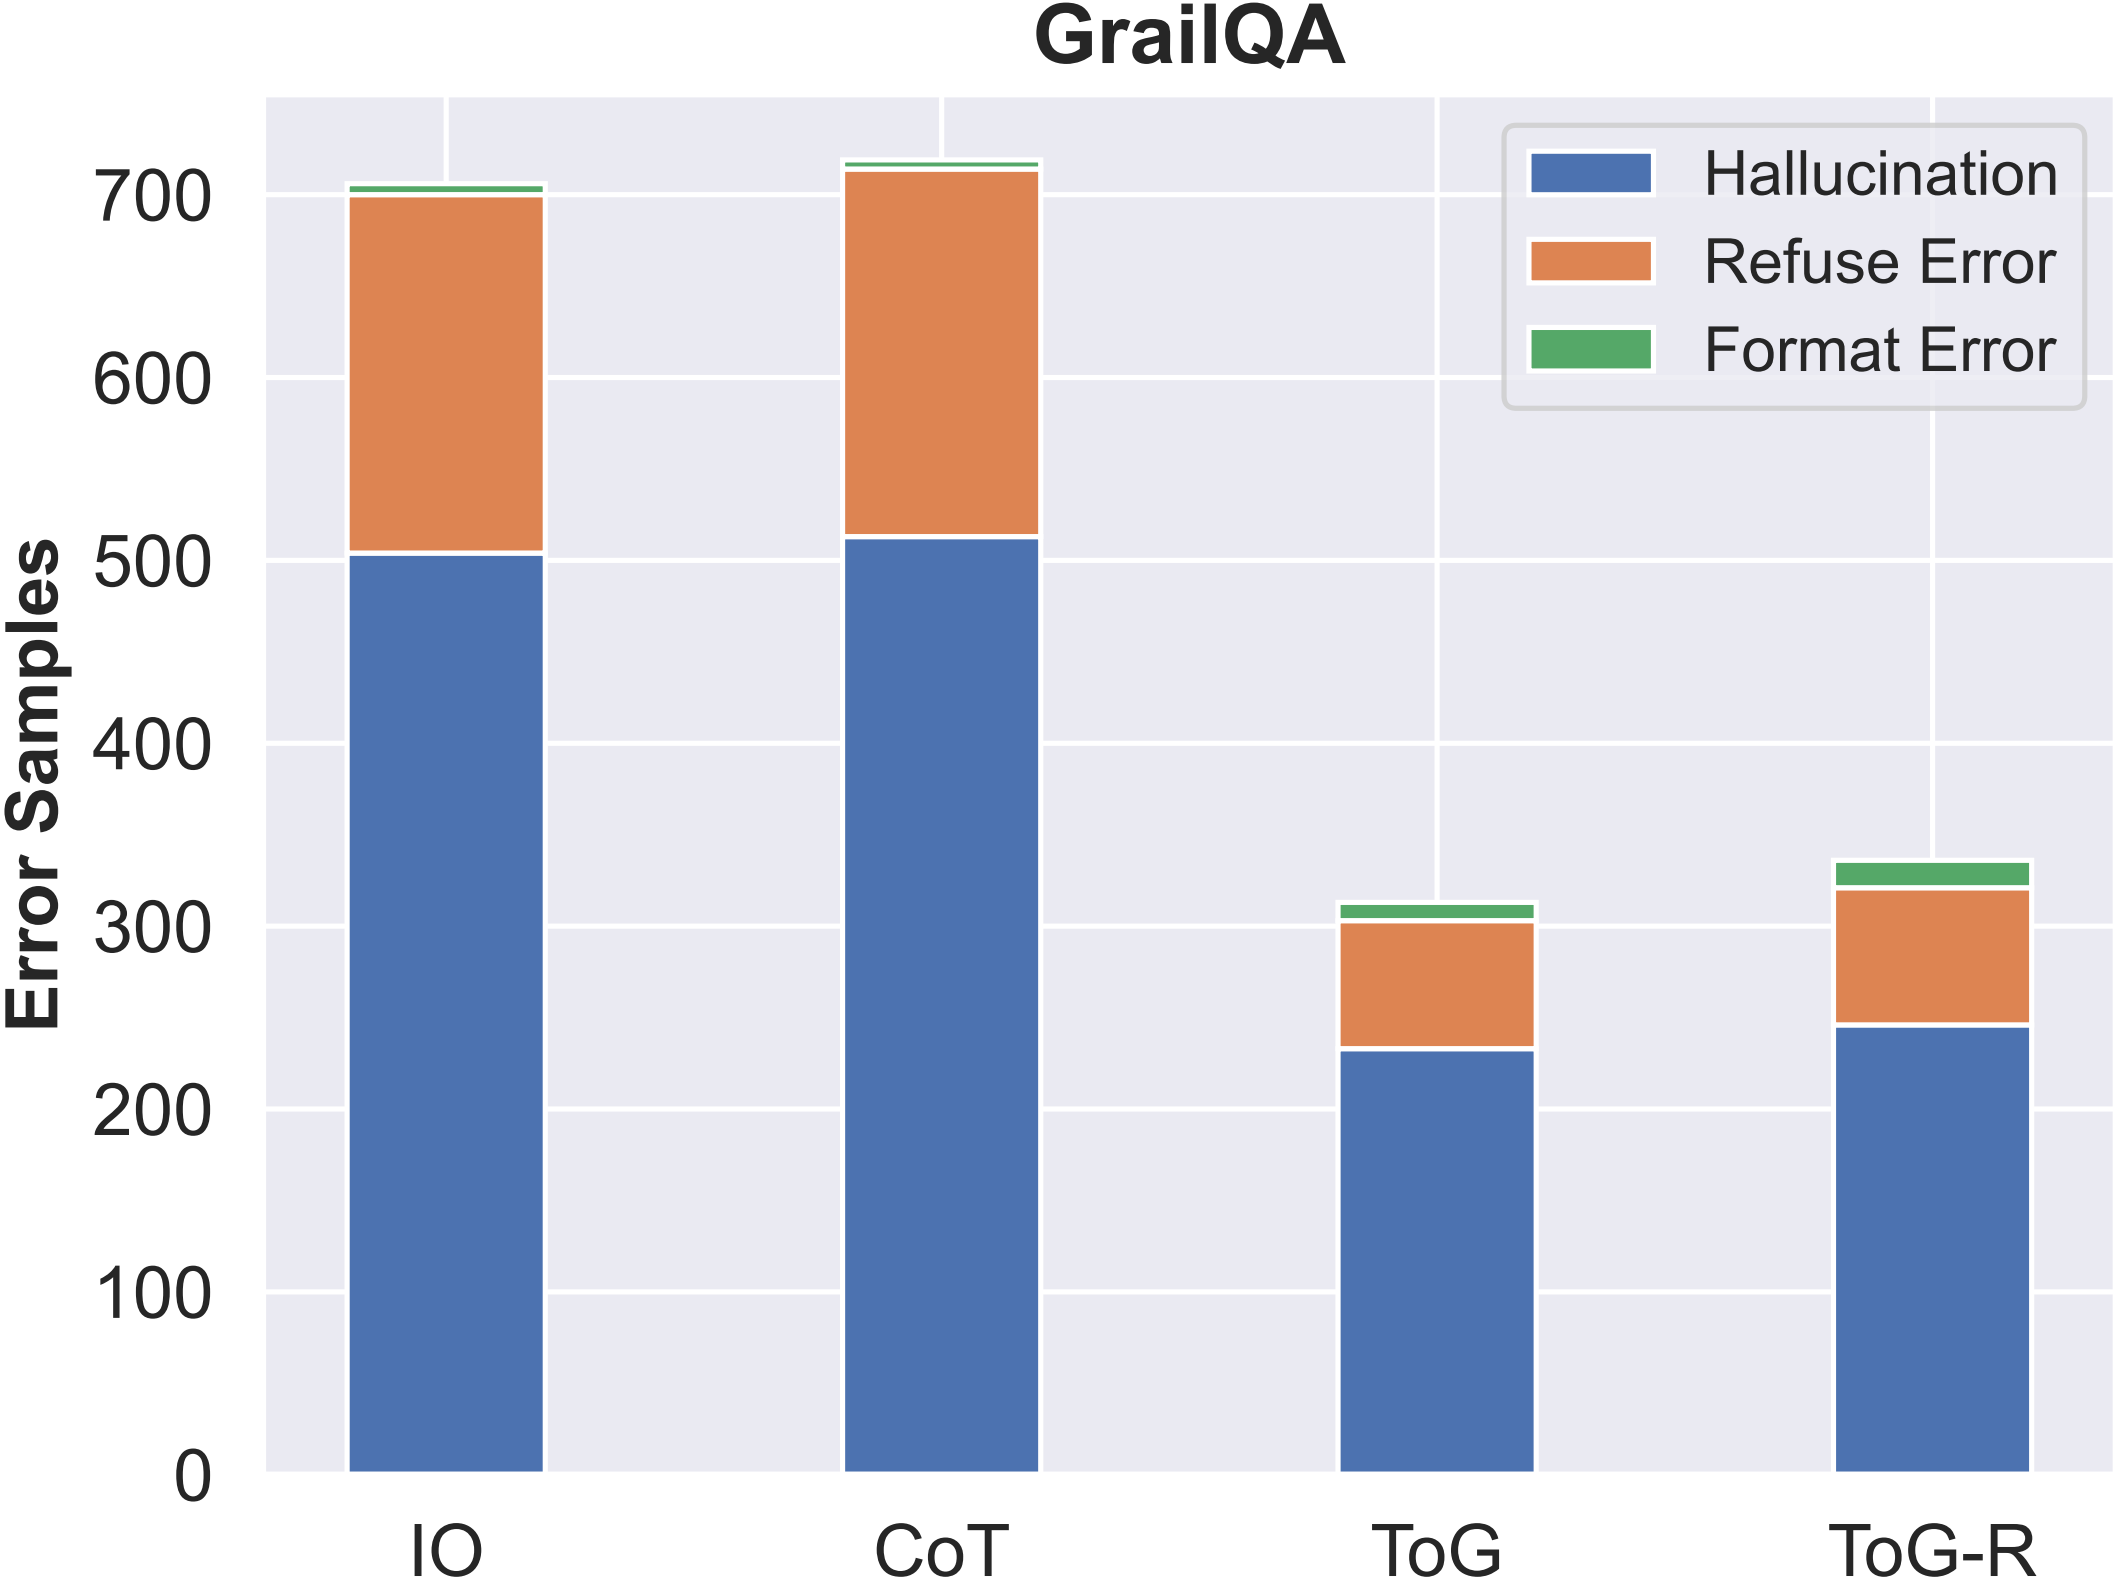
\includegraphics[width=\textwidth]{img/error_bar_grailqa.png}
    \end{subfigure}
    \caption{The erroneous instances and categories in the CWQ, WebQSP, and GrailQA of IO, CoT, and ToG.}
    \label{fig: error_analysis}
\end{figure}



\begin{wraptable}{r}{0.4\textwidth}
\centering
\resizebox{\linewidth}{!}{
\begin{tabular}{llc}
\hline
       \textbf{Search Algorithm}    & \textbf{Dataset} &  \textbf{EM} \\ \hline
\multirow{2}{*}{Naive Beam Search} 

&  	 
 CWQ                    & 30.1		 \\
 &   
 WebQSP                  &  46.1	   \\ \hline
\multirow{2}{*}{TOG-R}                 &  CWQ           &  59.2  \\ 
 &  WebQSP           &  75.1  \\\hline
\multirow{2}{*}{TOG}                 &  CWQ           &  58.8  \\ 
 &  WebQSP           &  76.2  \\\hline
\end{tabular}	
}
\caption{The results of Naive Beam Search, ToG methods on CWQ and WebQSP.}
\label{tab: diff_search_algo}
\end{wraptable}
\paragraph{Difference with Naive Beam Search}
ToG is slightly different from the beam search. ToG uses the top-$N$ reasoning paths as evidence while the naive beam search chooses the most plausible path as the only reasoning path. We conduct naive top1-beam search methods for ToG on CWQ and WebQSP. For each depth of the ToG, we choose the reasoning path with the highest plausibility, to evaluate if the current reasoning path is sufficient to answer the questions. The experiment results are shown in Table \ref{tab: diff_search_algo}. In naive beam search, the calibration error accumulates along the inference, leading to the instability of the final result.
We believe that ToG can partially alleviate this issue by considering the top-$N$ reasoning paths.



\subsection{Result Analysis}\label{sec: analysis}
We conduct a detailed analysis on the answers generated by ToG and ToG-R.

\paragraph{Error Analysis}
We considered three types of errors: (1) Hallucination error, (2) Refuse error \footnote{LLM will refuse to answer due to lack of information.}, and (3) Format error. The distribution is shown in Figure \ref{fig: error_analysis}. Our approach has significantly reduced the hallucination and refusal to answer error types in IO and CoT. For GrailQA, ToG even reduces these types of errors by 50\% and 60\%, respectively. Moreover, in ToG's error samples, there are still many instances of hallucination and refusal to answer errors. This is because the current search depth and width are both set to 3. By increasing the search depth and width, these error instances will further decrease (refer to Section \ref{sec: depth_breadth}). Furthermore, we currently generalize incorrect answers as hallucinations, but there are various categories within hallucinations, which we won't discuss in this paper. Additionally, after applying ToG, there's a slight increase in samples with format errors. This result shows that the explored paths lead to a noticeable increase in the tokens, sometimes even exceeding the maximum output limit. However, the error rate from this issue is negligible (less than 3\%).



\paragraph{Evidence of Answers}
We conducted an analysis of the correctly answered samples in three datasets to investigate the evidence for LLM in generating answers as shown in Figure \ref{fig: evidence_answers}. Evidently, a significant portion of the answers are derived from the paths explored by ToG, while roughly 20\% rely exclusively on the intrinsic knowledge embedded within LLM's parameters for generating responses. It is worth noting that around 7\% of the correctly answered samples require a combination of knowledge from both the explored paths and LLM's inherent knowledge (as elaborated in Appendix Table \ref{table: case3}). This distinction sets our approach apart from traditional graph-based search methods, as it does not necessitate the path to encompass the node containing the correct answer entirely. Instead, the explored paths supplement and reference LLM's inherent knowledge. The distribution of answer types for ToG-R is almost indistinguishable from that of ToG, proving the robustness of our approach. 


\begin{figure}[htbp]
    \centering
    \begin{subfigure}[b]{0.32\textwidth}
        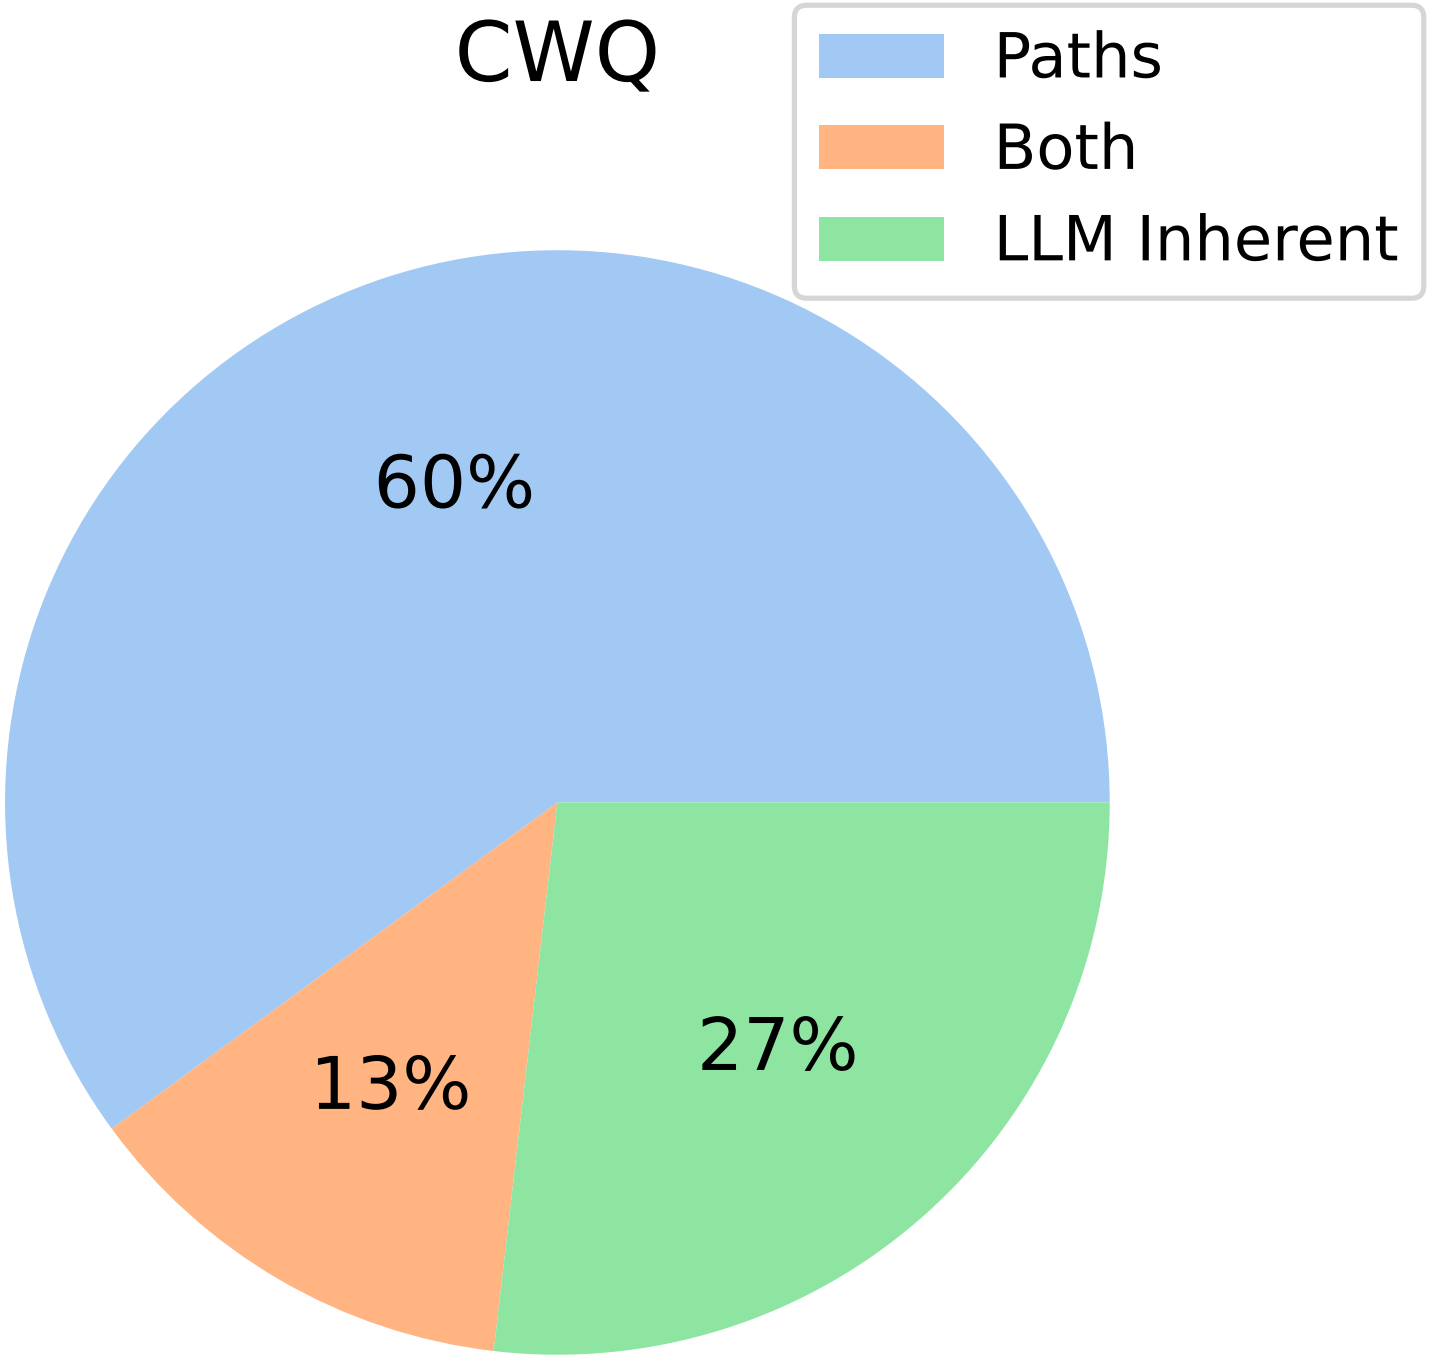
\includegraphics[width=\textwidth]{img/pie_cwq.png}
    \end{subfigure}
    \hfill
    \begin{subfigure}[b]{0.32\textwidth}
        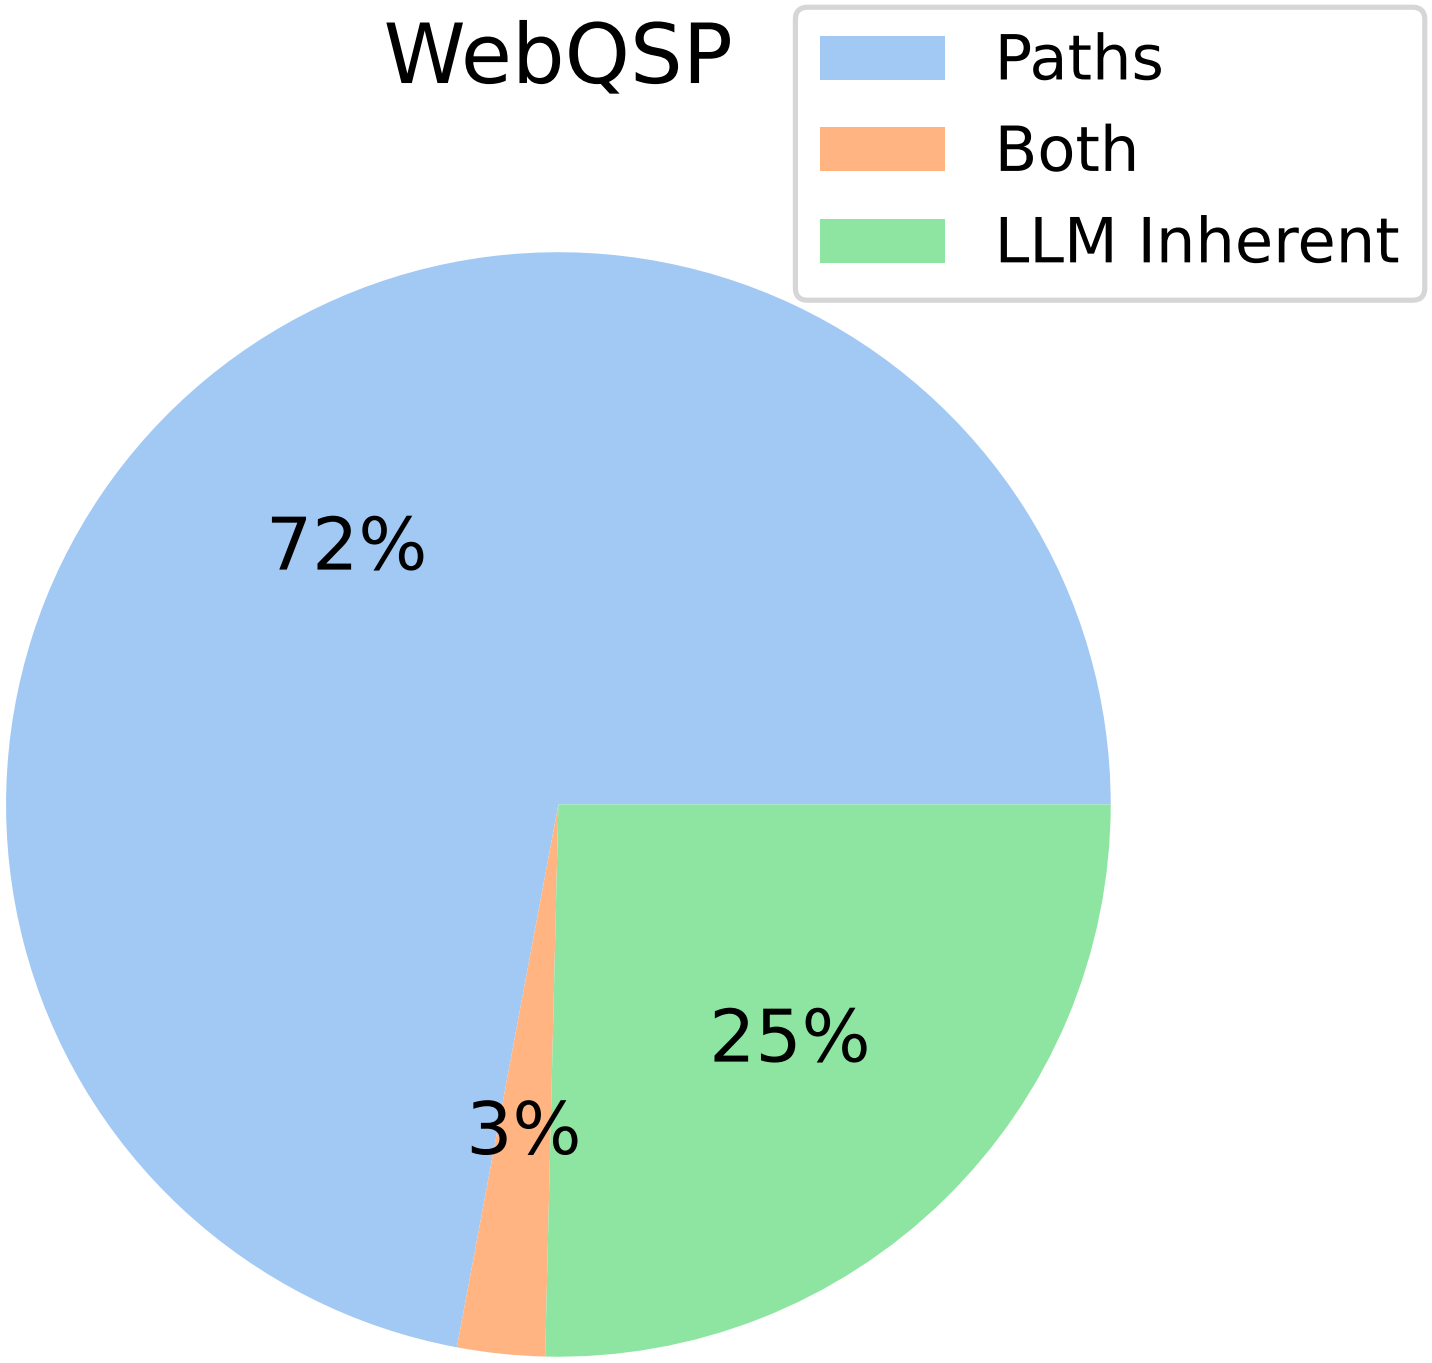
\includegraphics[width=\textwidth]{img/pie_webqsp.png}
    \end{subfigure}
    \hfill
    \begin{subfigure}[b]{0.32\textwidth}
        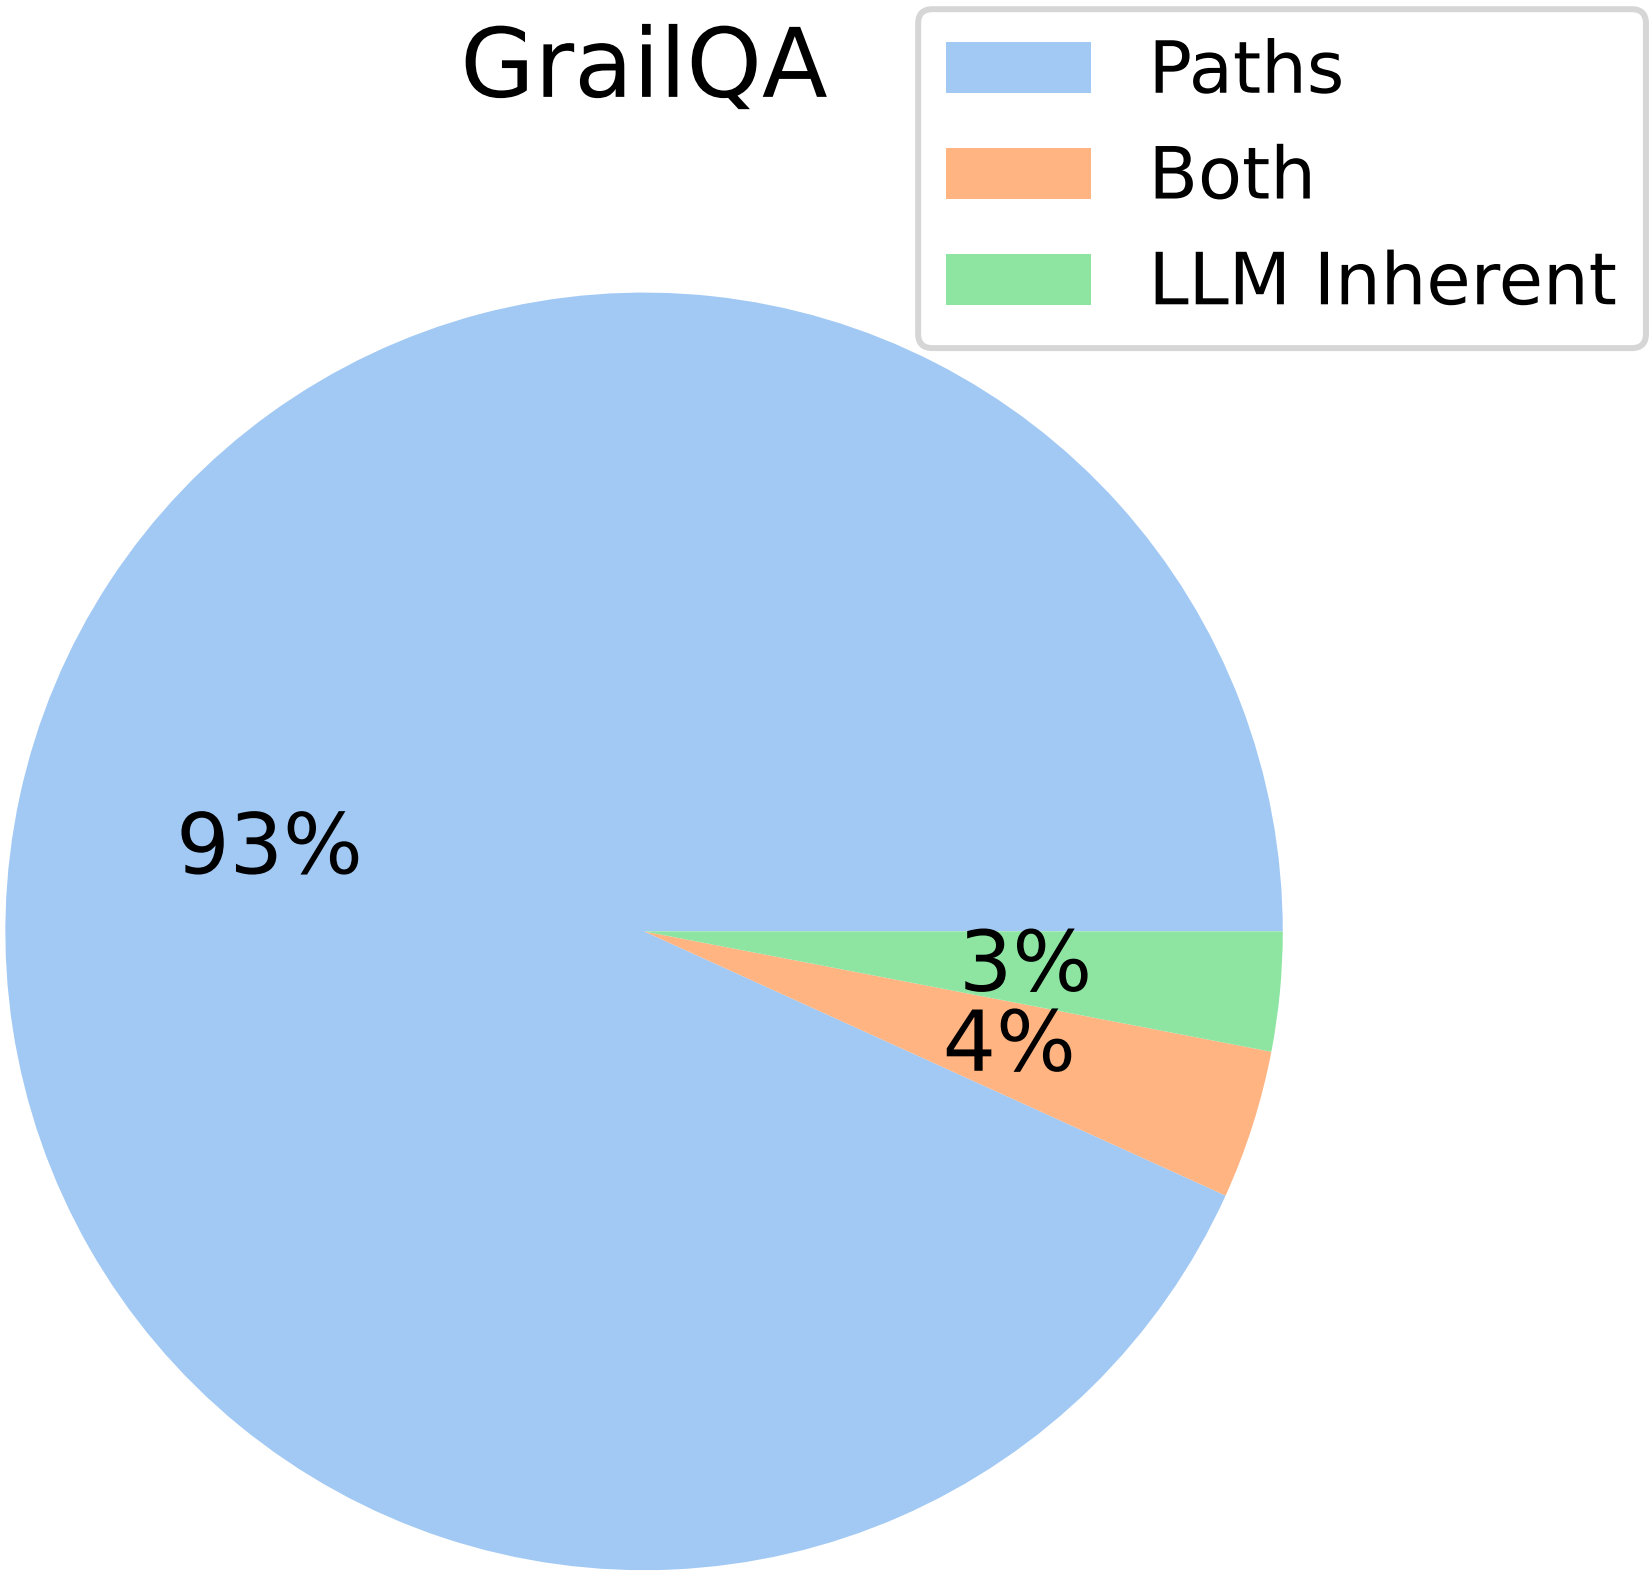
\includegraphics[width=\textwidth]{img/pie_grailqa.png}
    \end{subfigure}
    \caption{The proportions of ToG's evidence of answers on CWQ, WebQSP, and GrailQA datasets.}
    \label{fig: evidence_answers}
\end{figure}

\begin{figure}[htbp]
    \centering
    \begin{subfigure}[b]{0.32\textwidth}
        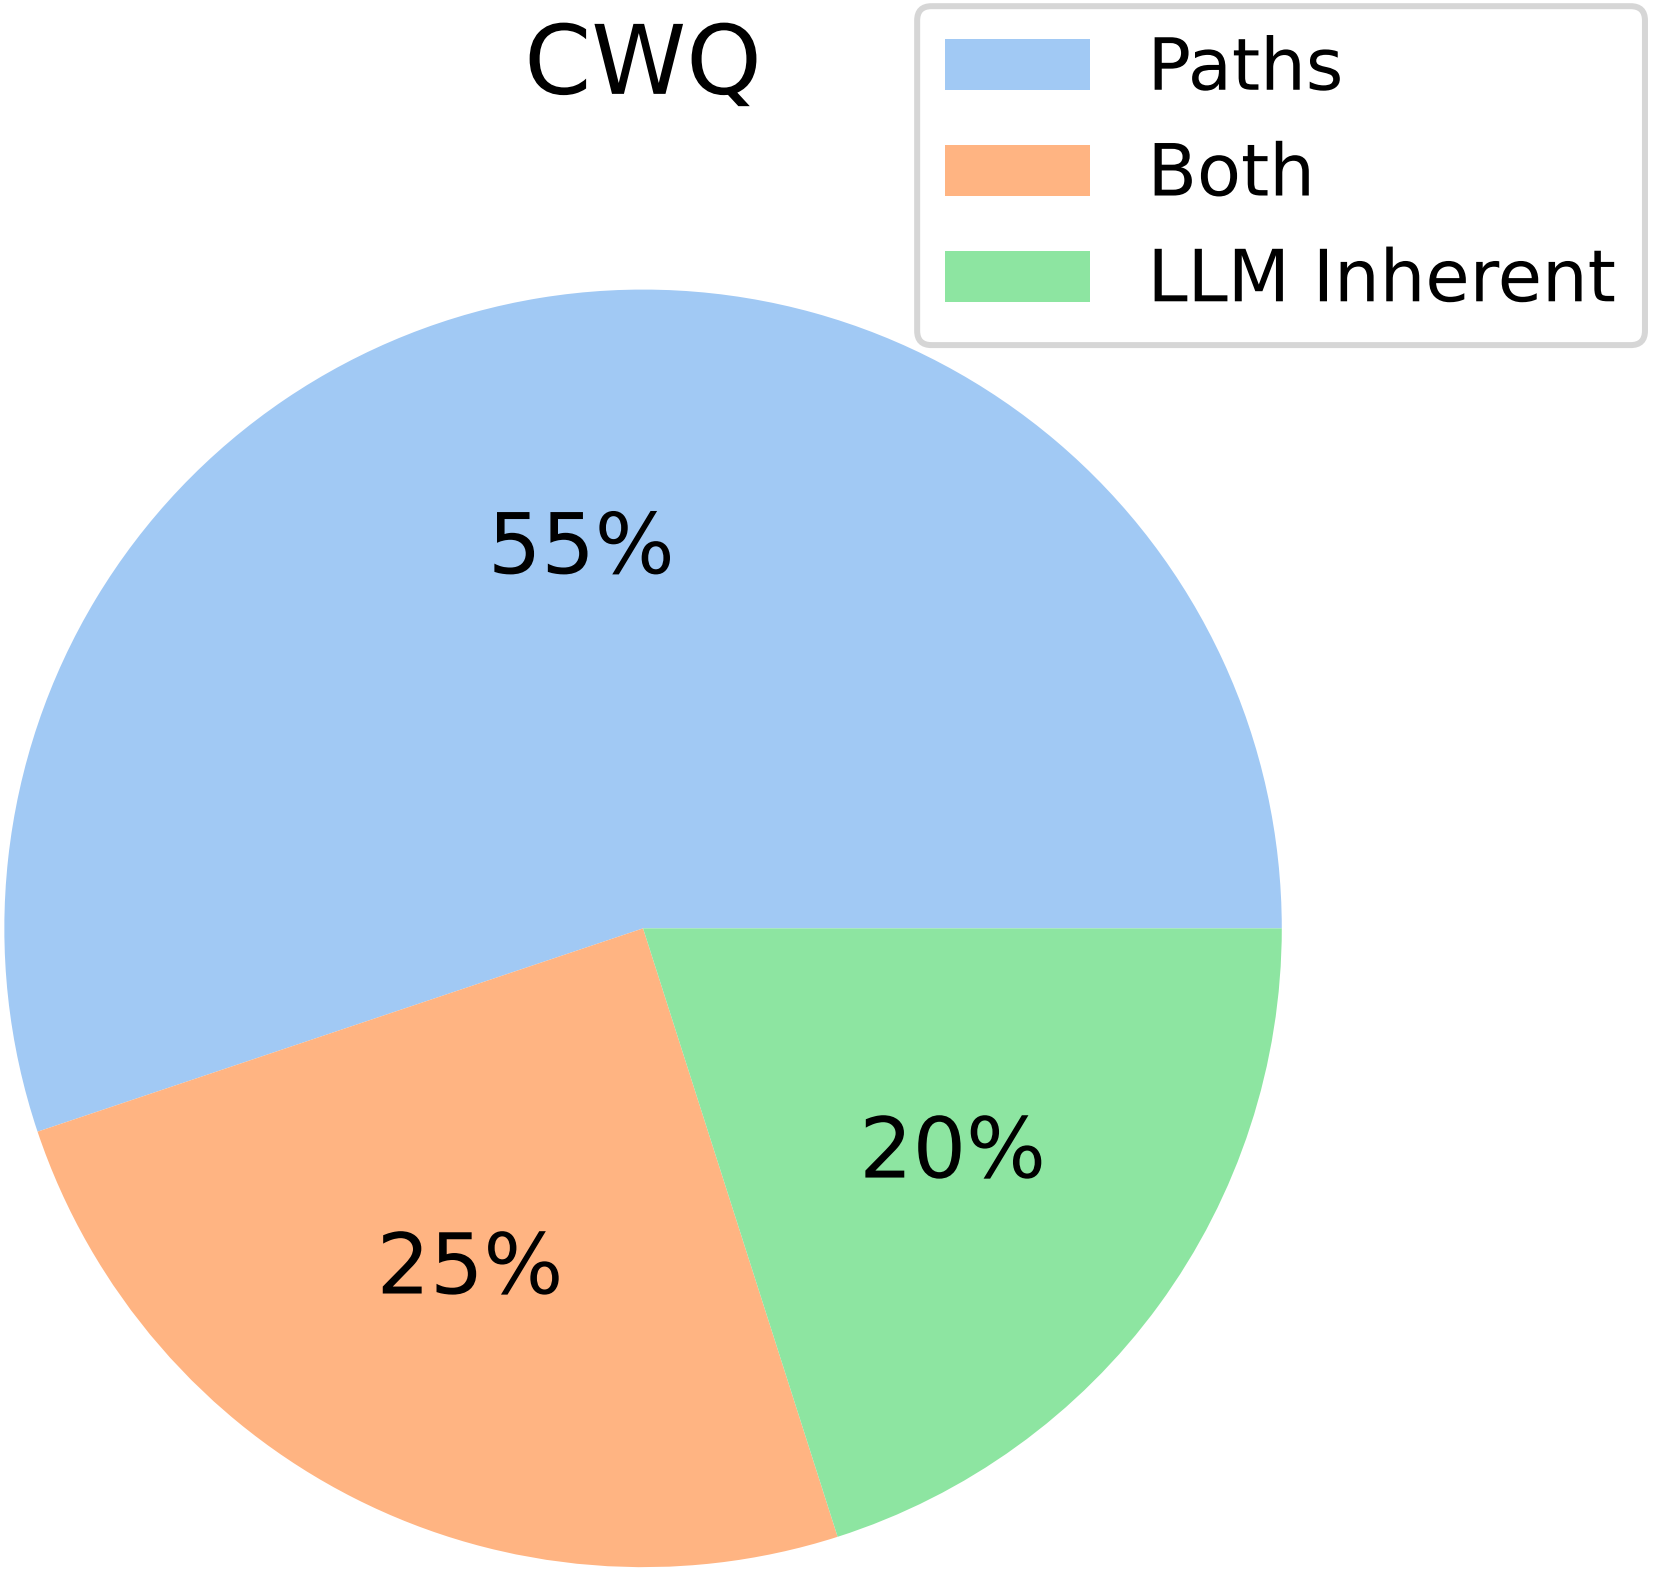
\includegraphics[width=\textwidth]{img/pie_cwq_togr.png}
    \end{subfigure}
    \hfill
    \begin{subfigure}[b]{0.32\textwidth}
        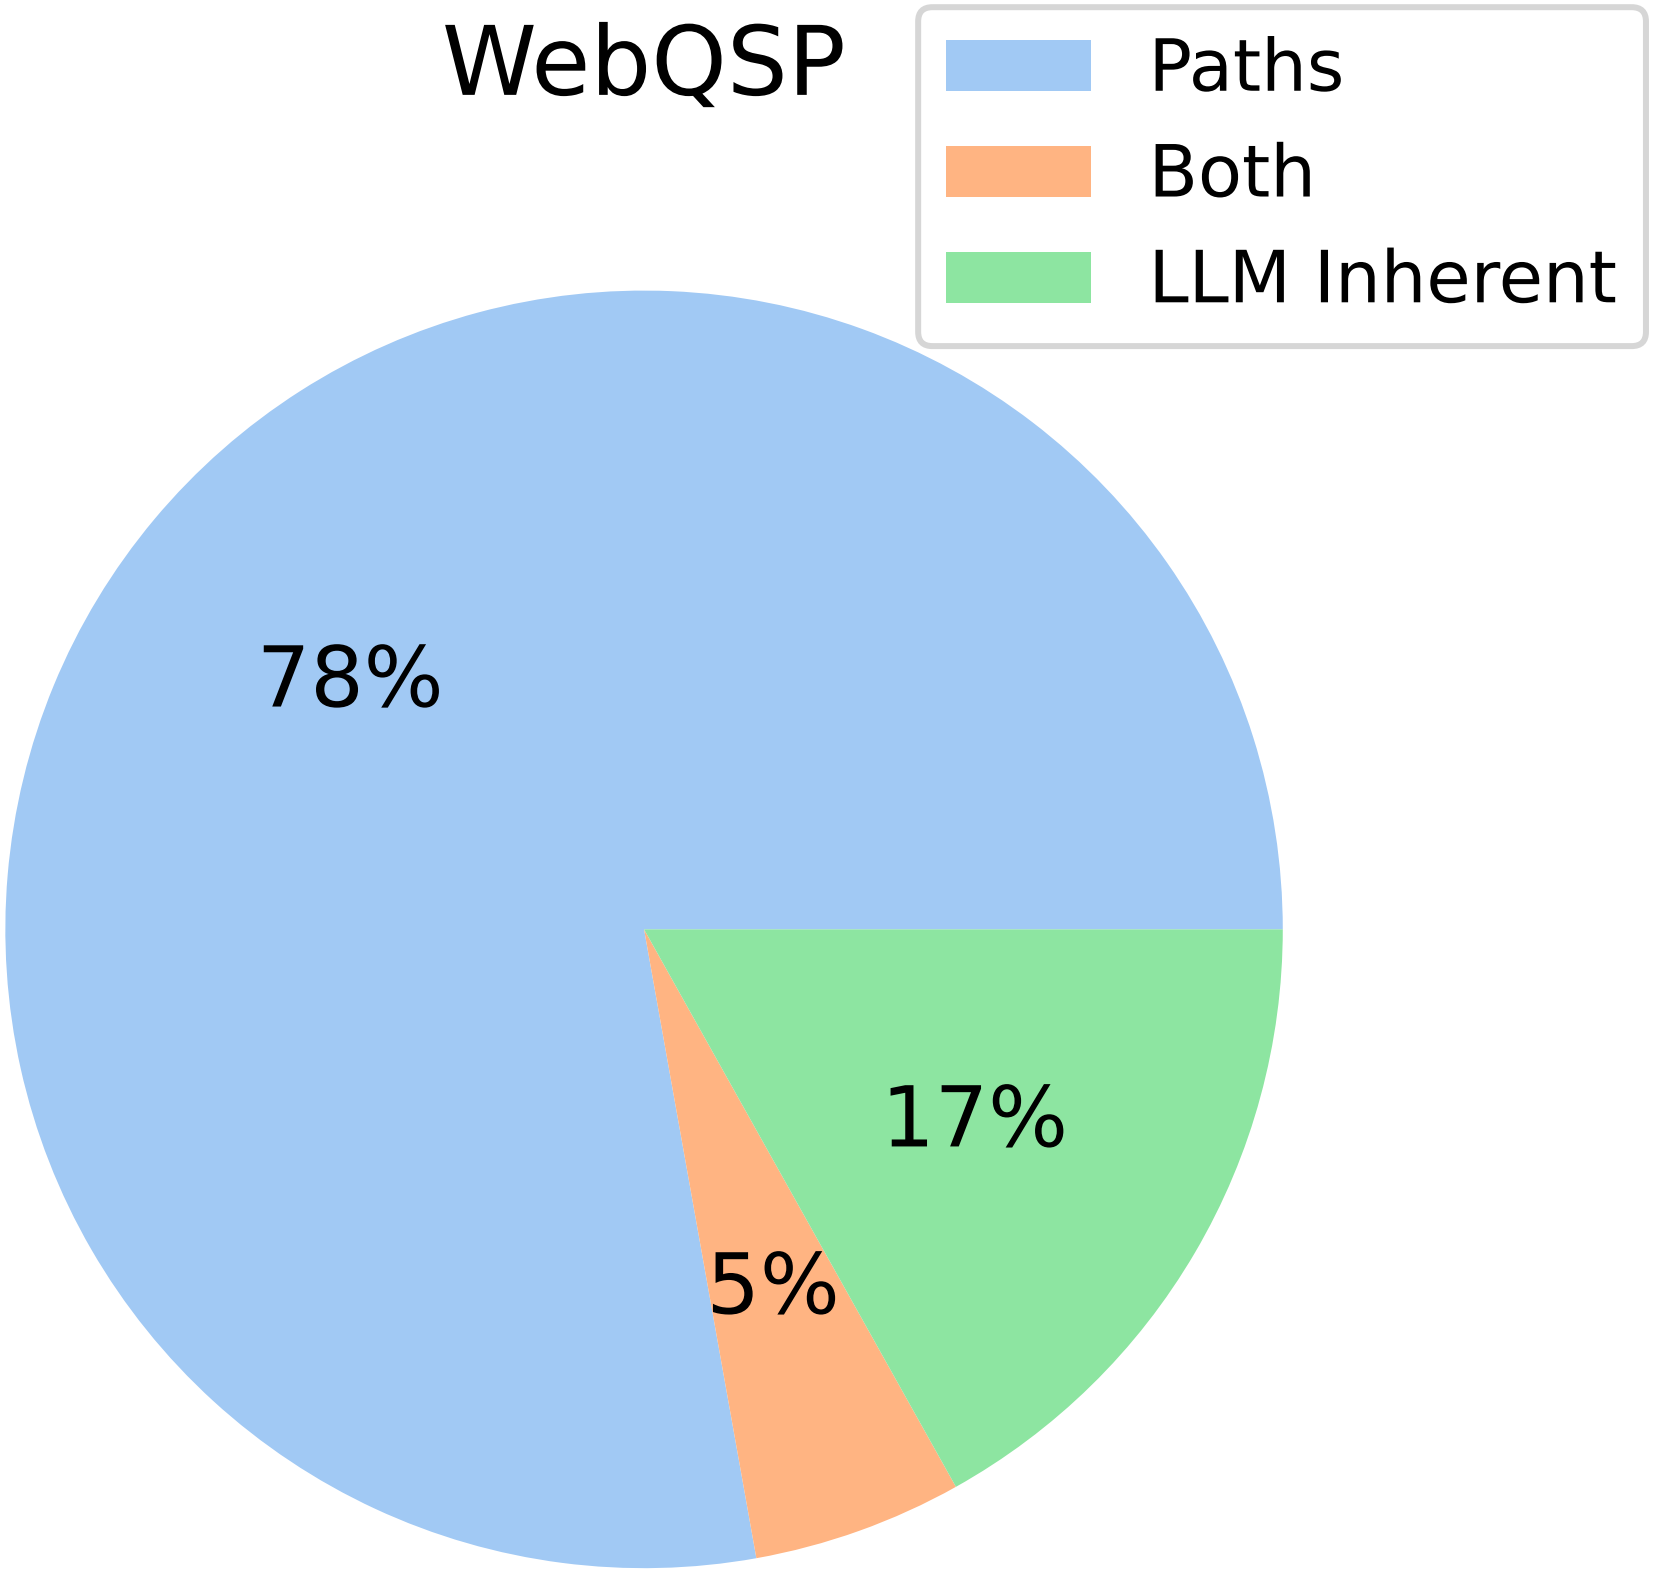
\includegraphics[width=\textwidth]{img/pie_webqsp_togr.png}
    \end{subfigure}
    \hfill
    \begin{subfigure}[b]{0.32\textwidth}
        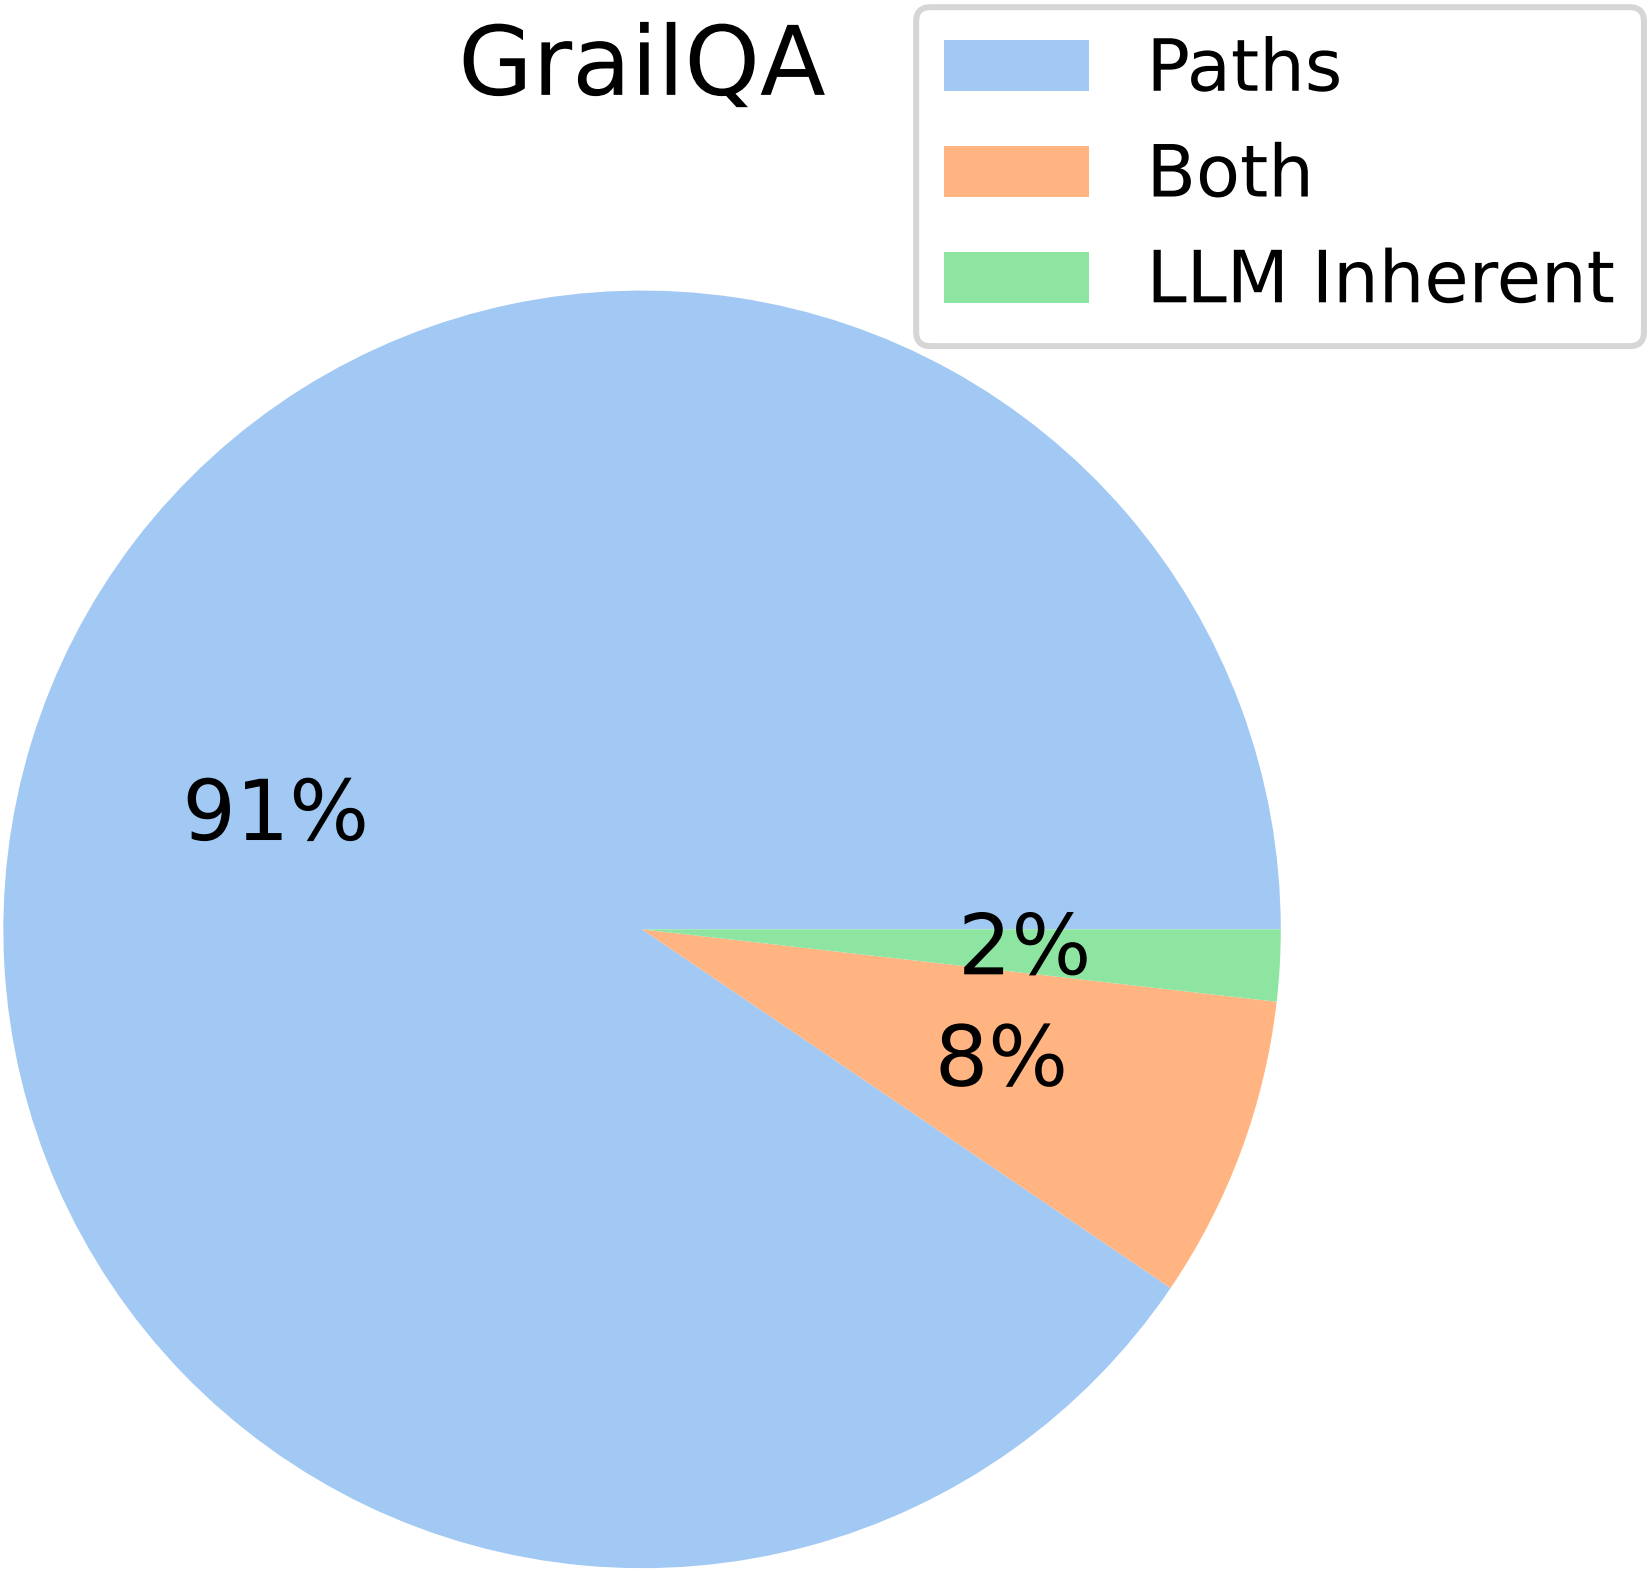
\includegraphics[width=\textwidth]{img/pie_grailqa_togr.png}
    \end{subfigure}
    \caption{The explored path overlap ratio of ToG-R on CWQ, WebQSP, and GrailQA datasets.}
    \label{fig: evidence_answers_togr}
\end{figure}



\paragraph{The Overlap Ratio between the Explored Paths and Ground-truth Paths}
\label{sec: overlap_ratio}
We also conduct an analysis of the correctly answered samples in three datasets to investigate the ratio of overlap between the paths explored by ToG and the ground-truth path in SPARQL. The definition of overlap ratio is the ratio of overlapping paths to the total number of relations in ground-truth SPARQL:
$$\frac{\text{Count}(\text{Rel}(\text{Paths}) \cap \text{Rel}(\text{SPARQL})) }{\text{Count}(\text{Rel}(\text{SPARQL}))}$$
where \text{Rel}(*) denotes all the unduplicated relations in the "*" and Count(*) denotes the number of "*"\footnote{We approximately calculate the length of a path by counting the number of relations in the ground-truth SPARQL.}. Figure \ref{fig: path_schematic} is a path schematic which takes the case shown in Table \ref{table: case4} for example.
It can be observed from Figure \ref{fig: overlap_ratio} that the paths explored by ToG are identical to the golden paths of an average of 30\% correct samples, while the paths of an average of 21\% correct samples are completely different from the golden path. This indicates that ToG has successfully explored a completely and approximately new path in the knowledge graph space to reach the final answer entity. For ToG-R, the disparity between the two is primarily evident in the CWQ dataset, where the percentage of intervals (25,50] in ToG results is quite significant (nearly 40\%), whereas ToG-R results tend to be more evenly distributed as shown in Figure \ref{fig: overlap_ratio_togr}. We contend that this discrepancy arises from the disregard of entity, thereby enhancing the diversity of explored relations. This represents a significant application of knowledge graph reasoning in academic research.

\begin{figure}
  \centering
  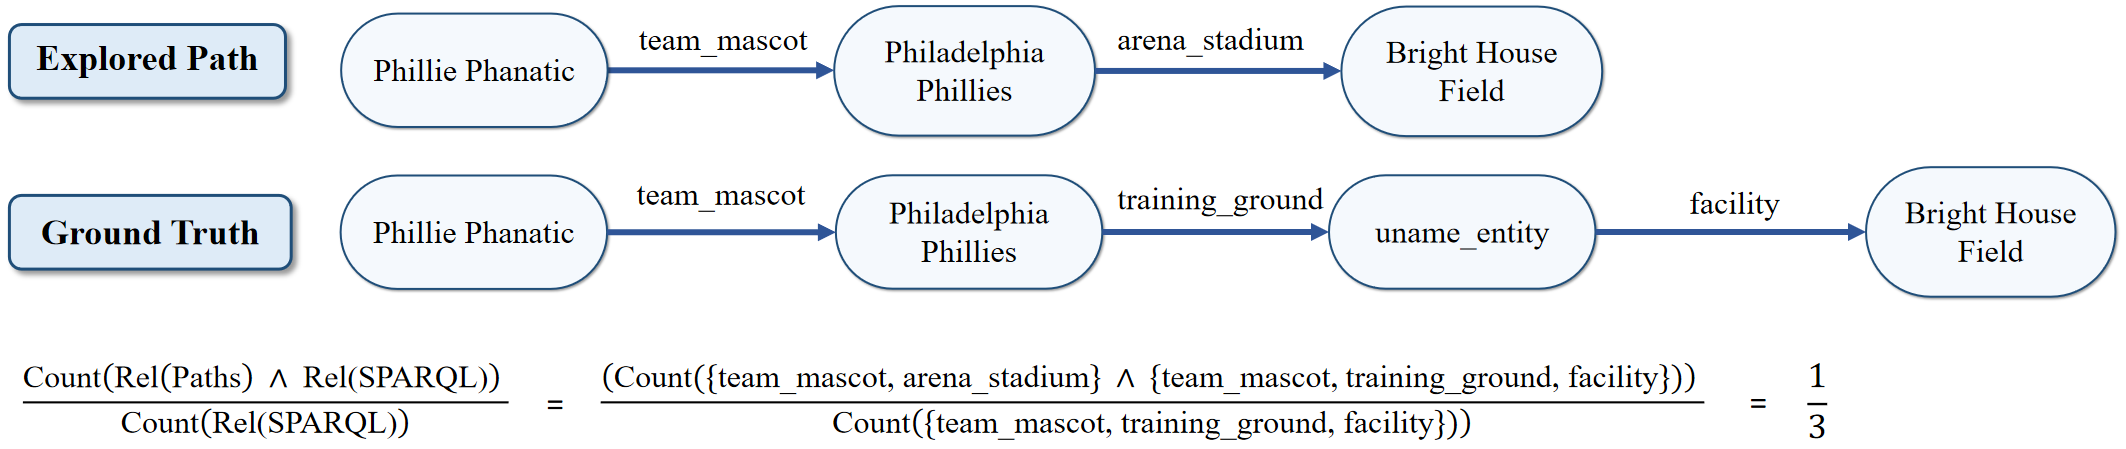
\includegraphics[width=0.95\textwidth]{img/link_overlap.png}
  \caption{Path schematic to calculate overlap.}
  \label{fig: path_schematic}
\end{figure}

\begin{figure}[htbp]
    \centering
    \begin{subfigure}[b]{0.32\textwidth}
        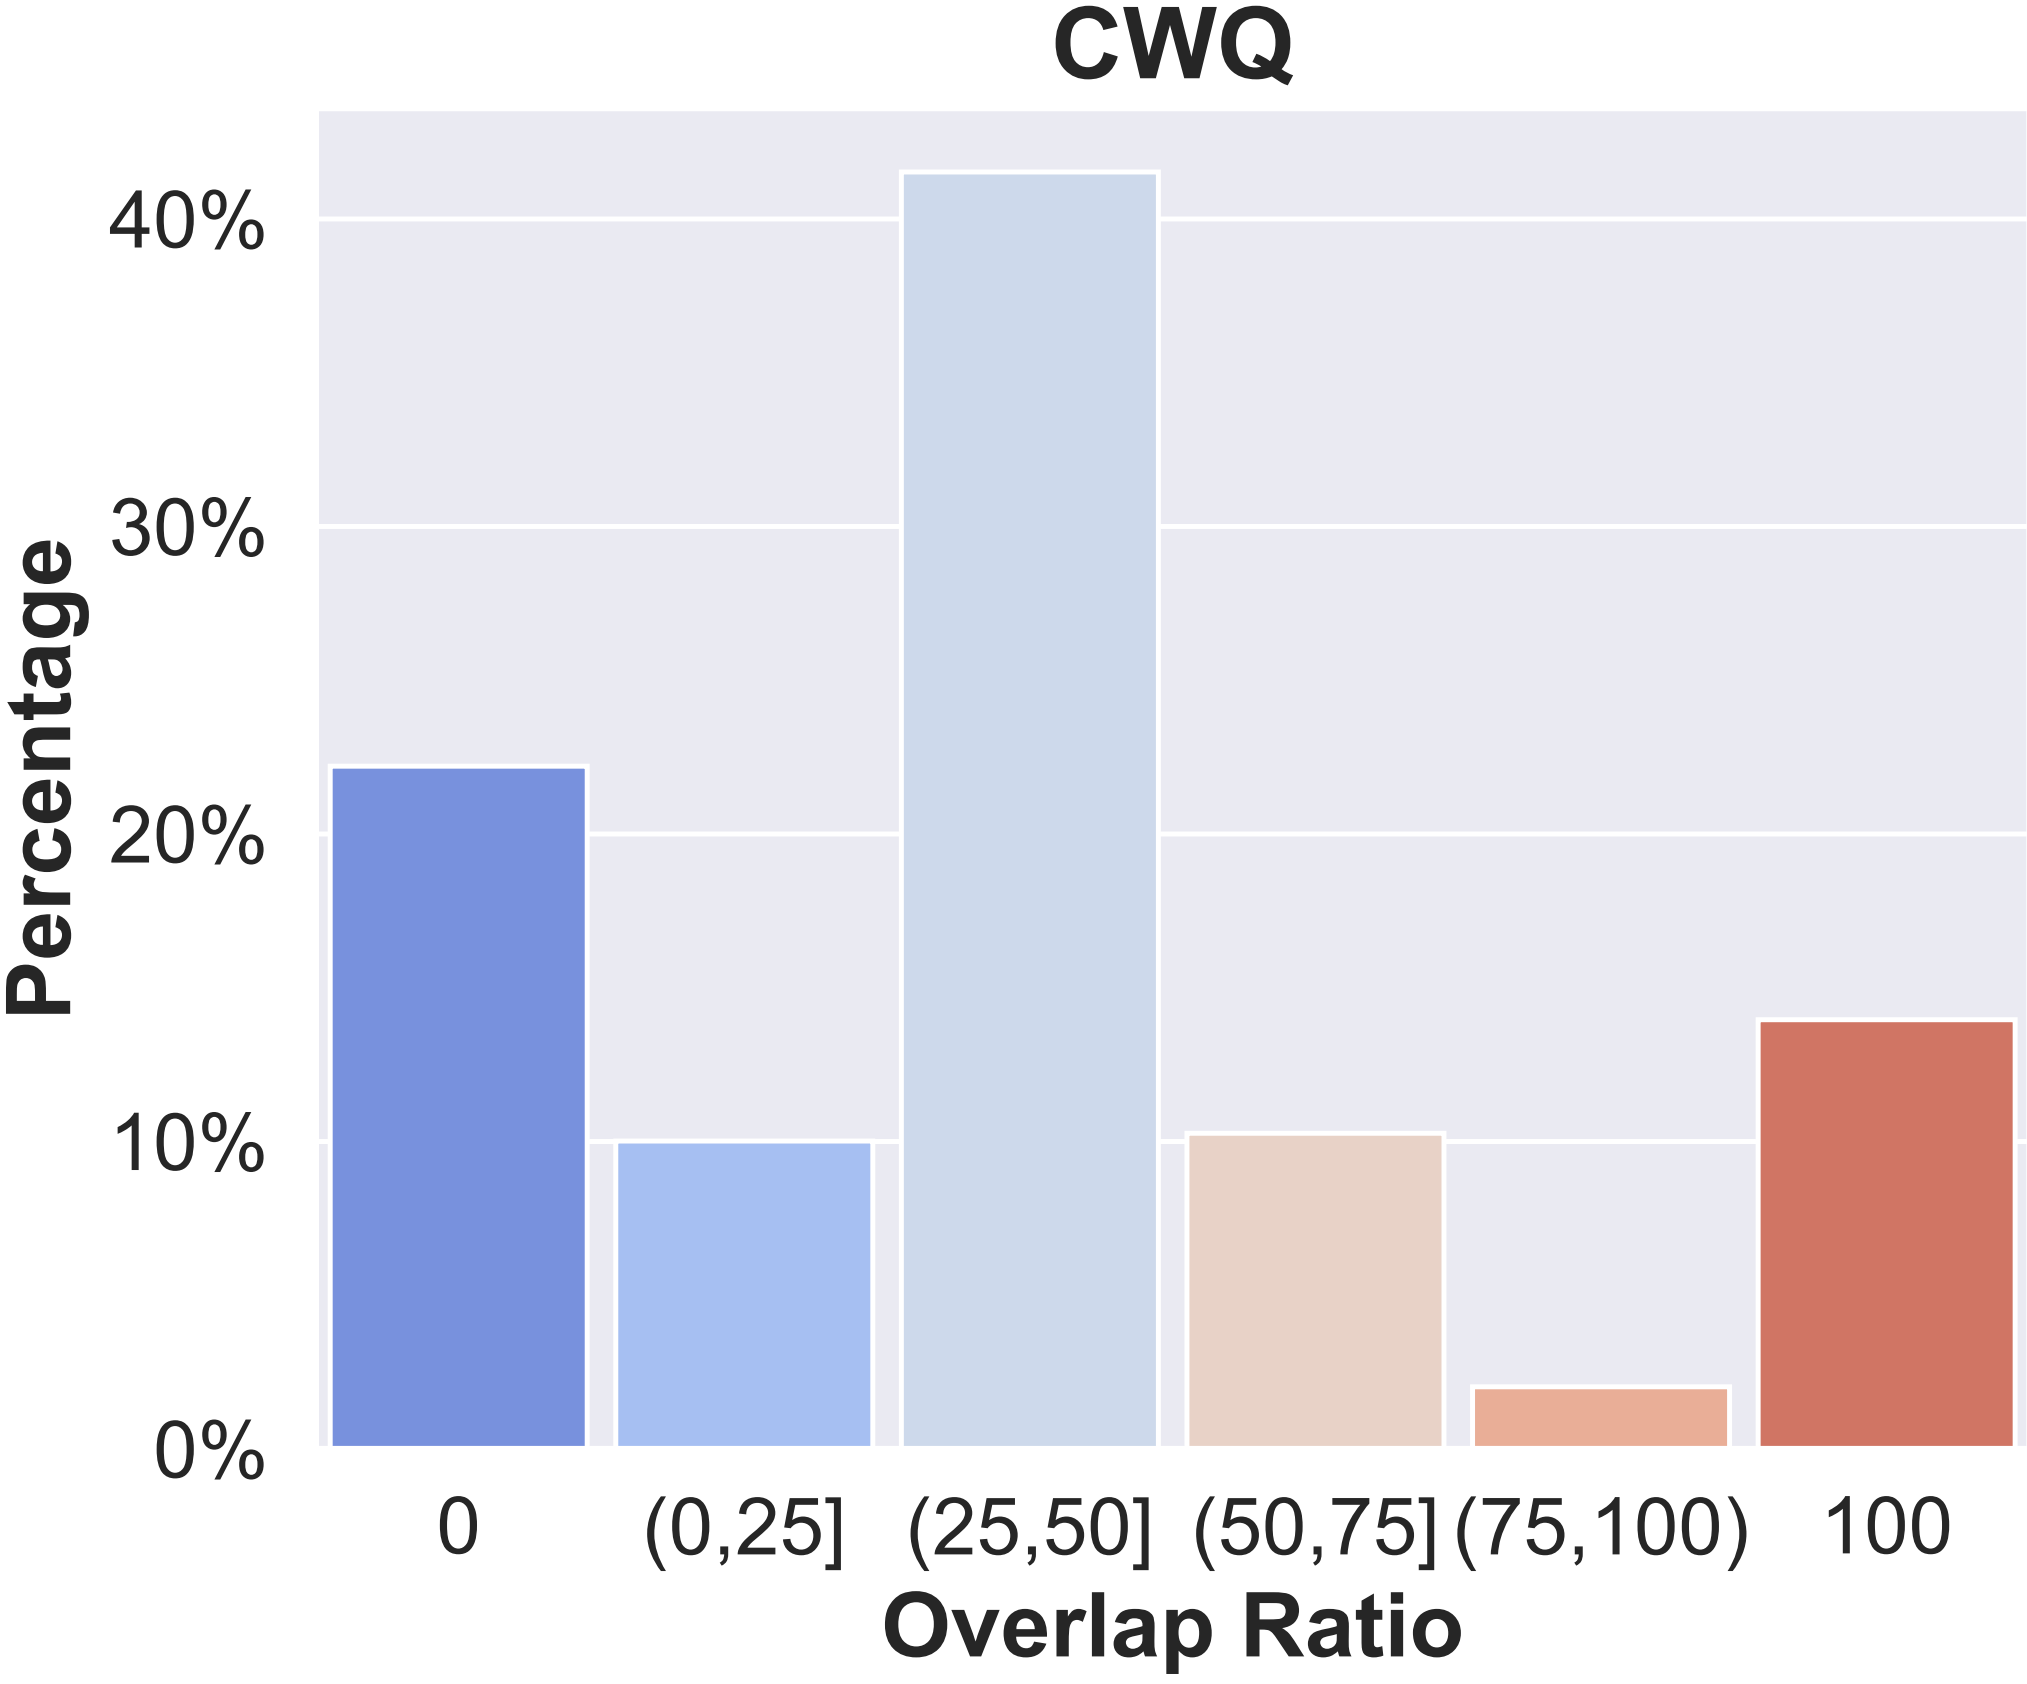
\includegraphics[width=\textwidth]{img/dis_cwq.png}
    \end{subfigure}
    \hfill
    \begin{subfigure}[b]{0.32\textwidth}
        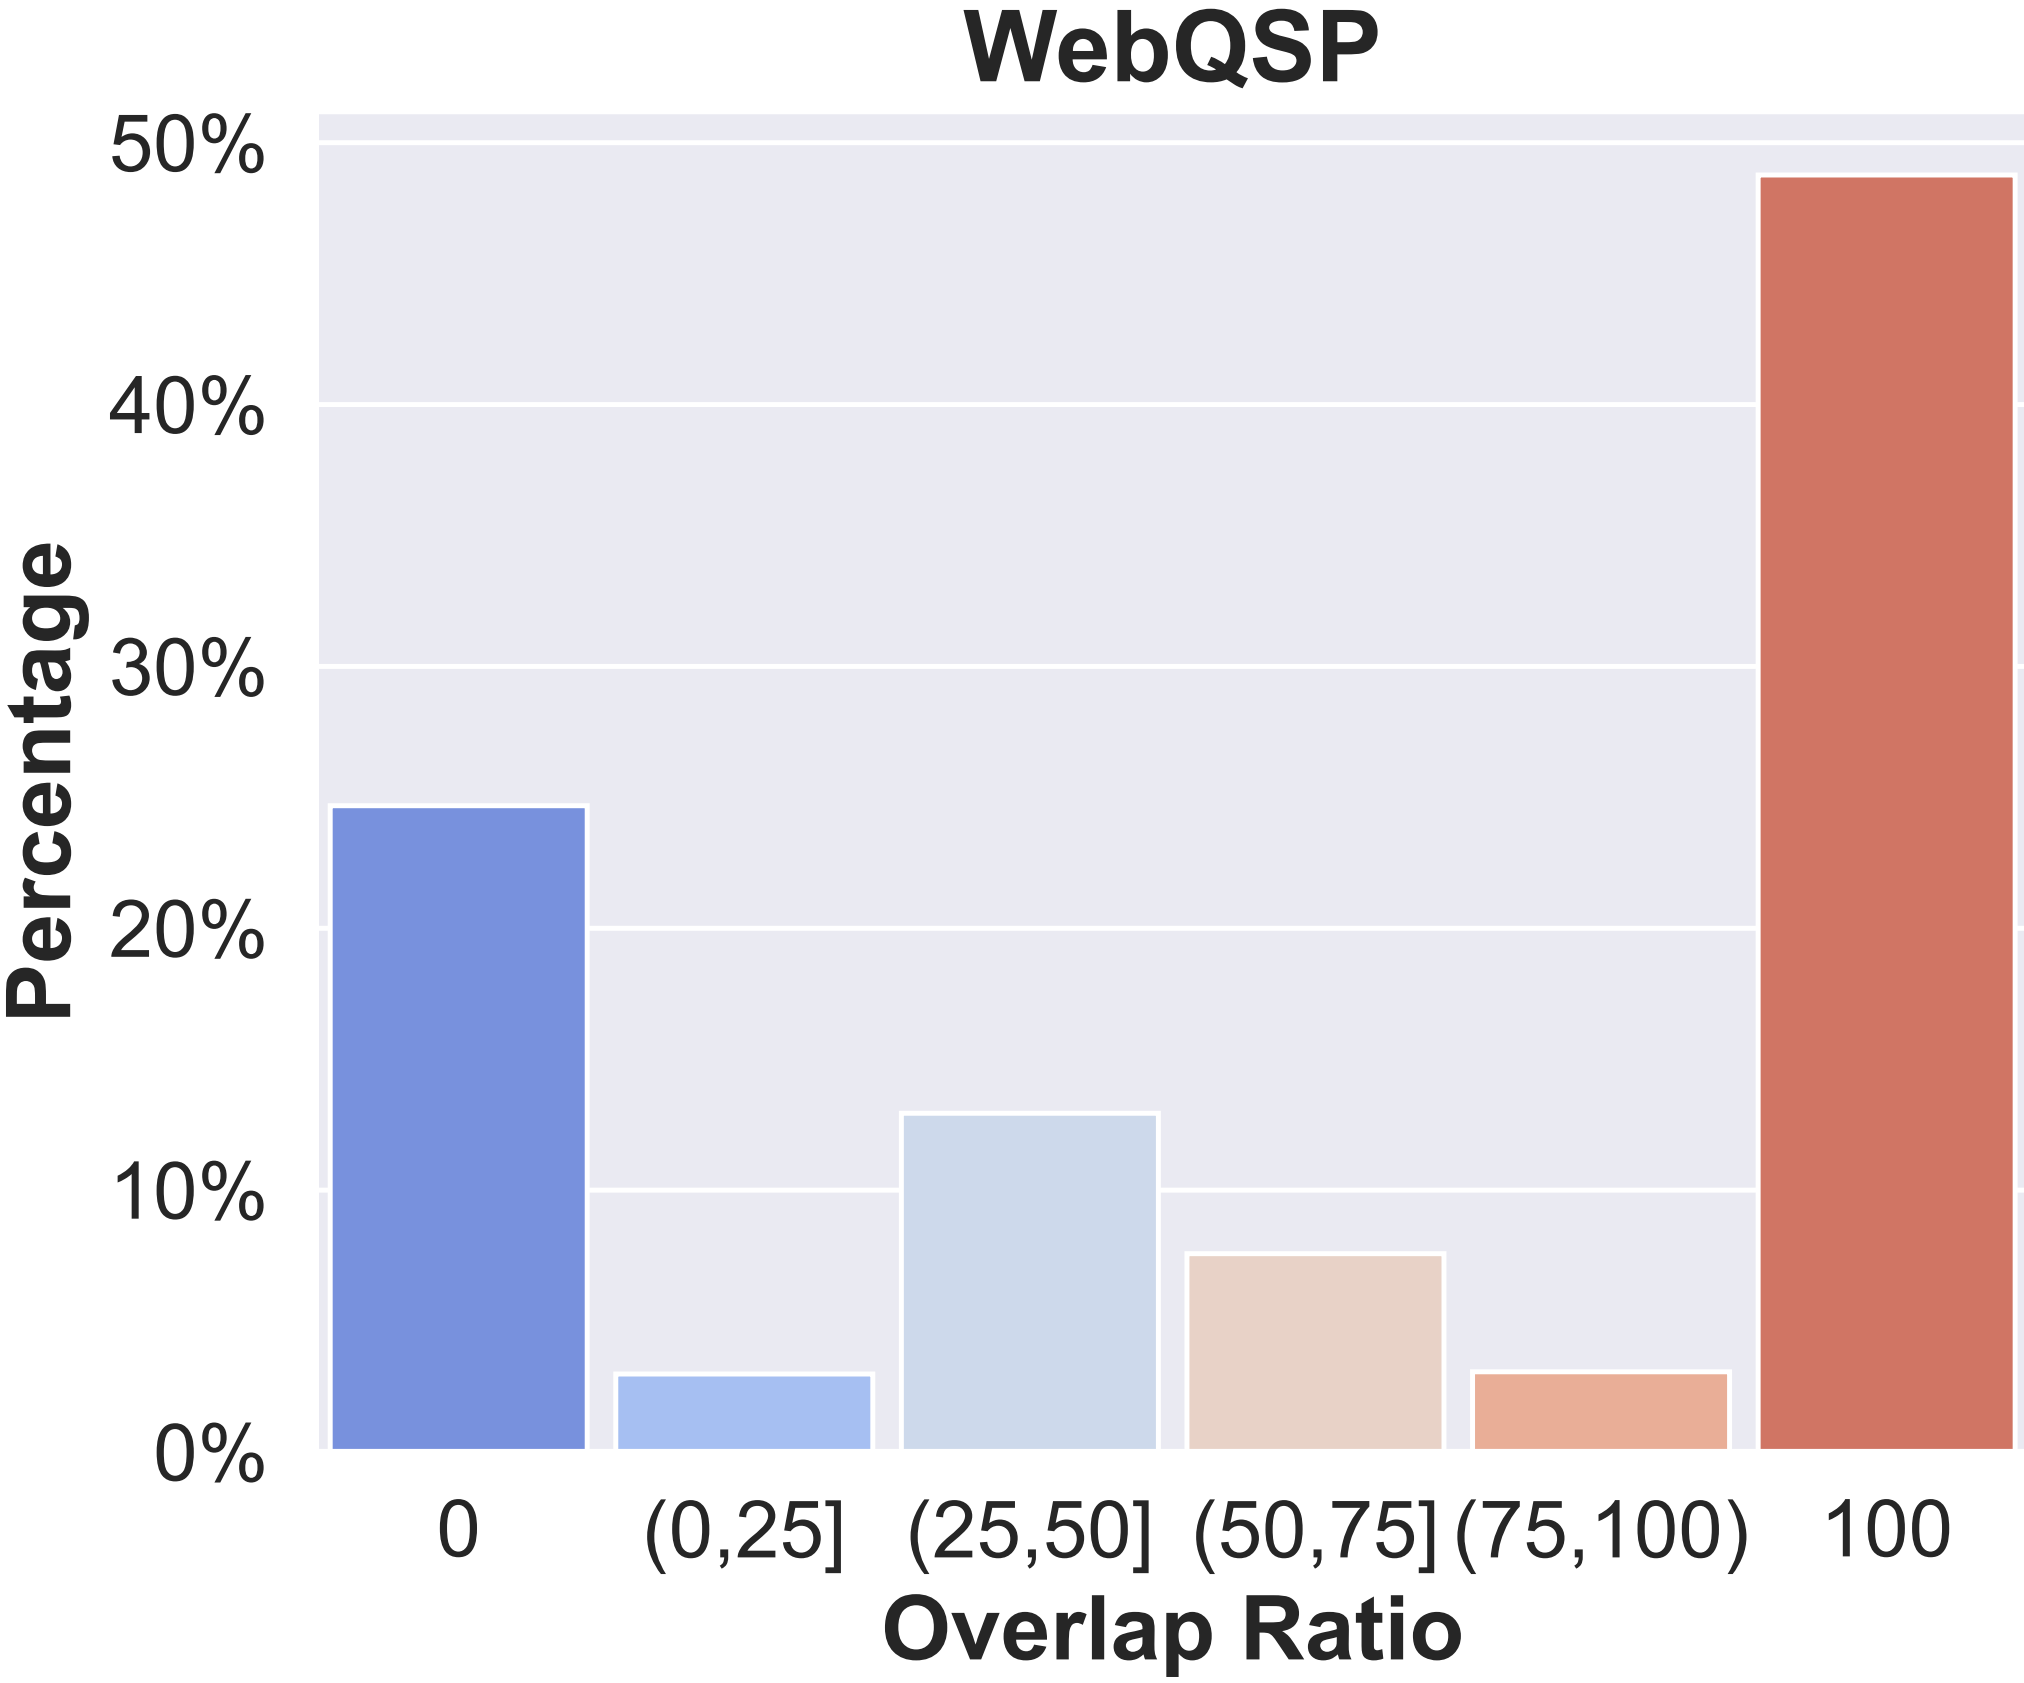
\includegraphics[width=\textwidth]{img/dis_webqsp.png}
    \end{subfigure}
    \hfill
    \begin{subfigure}[b]{0.32\textwidth}
        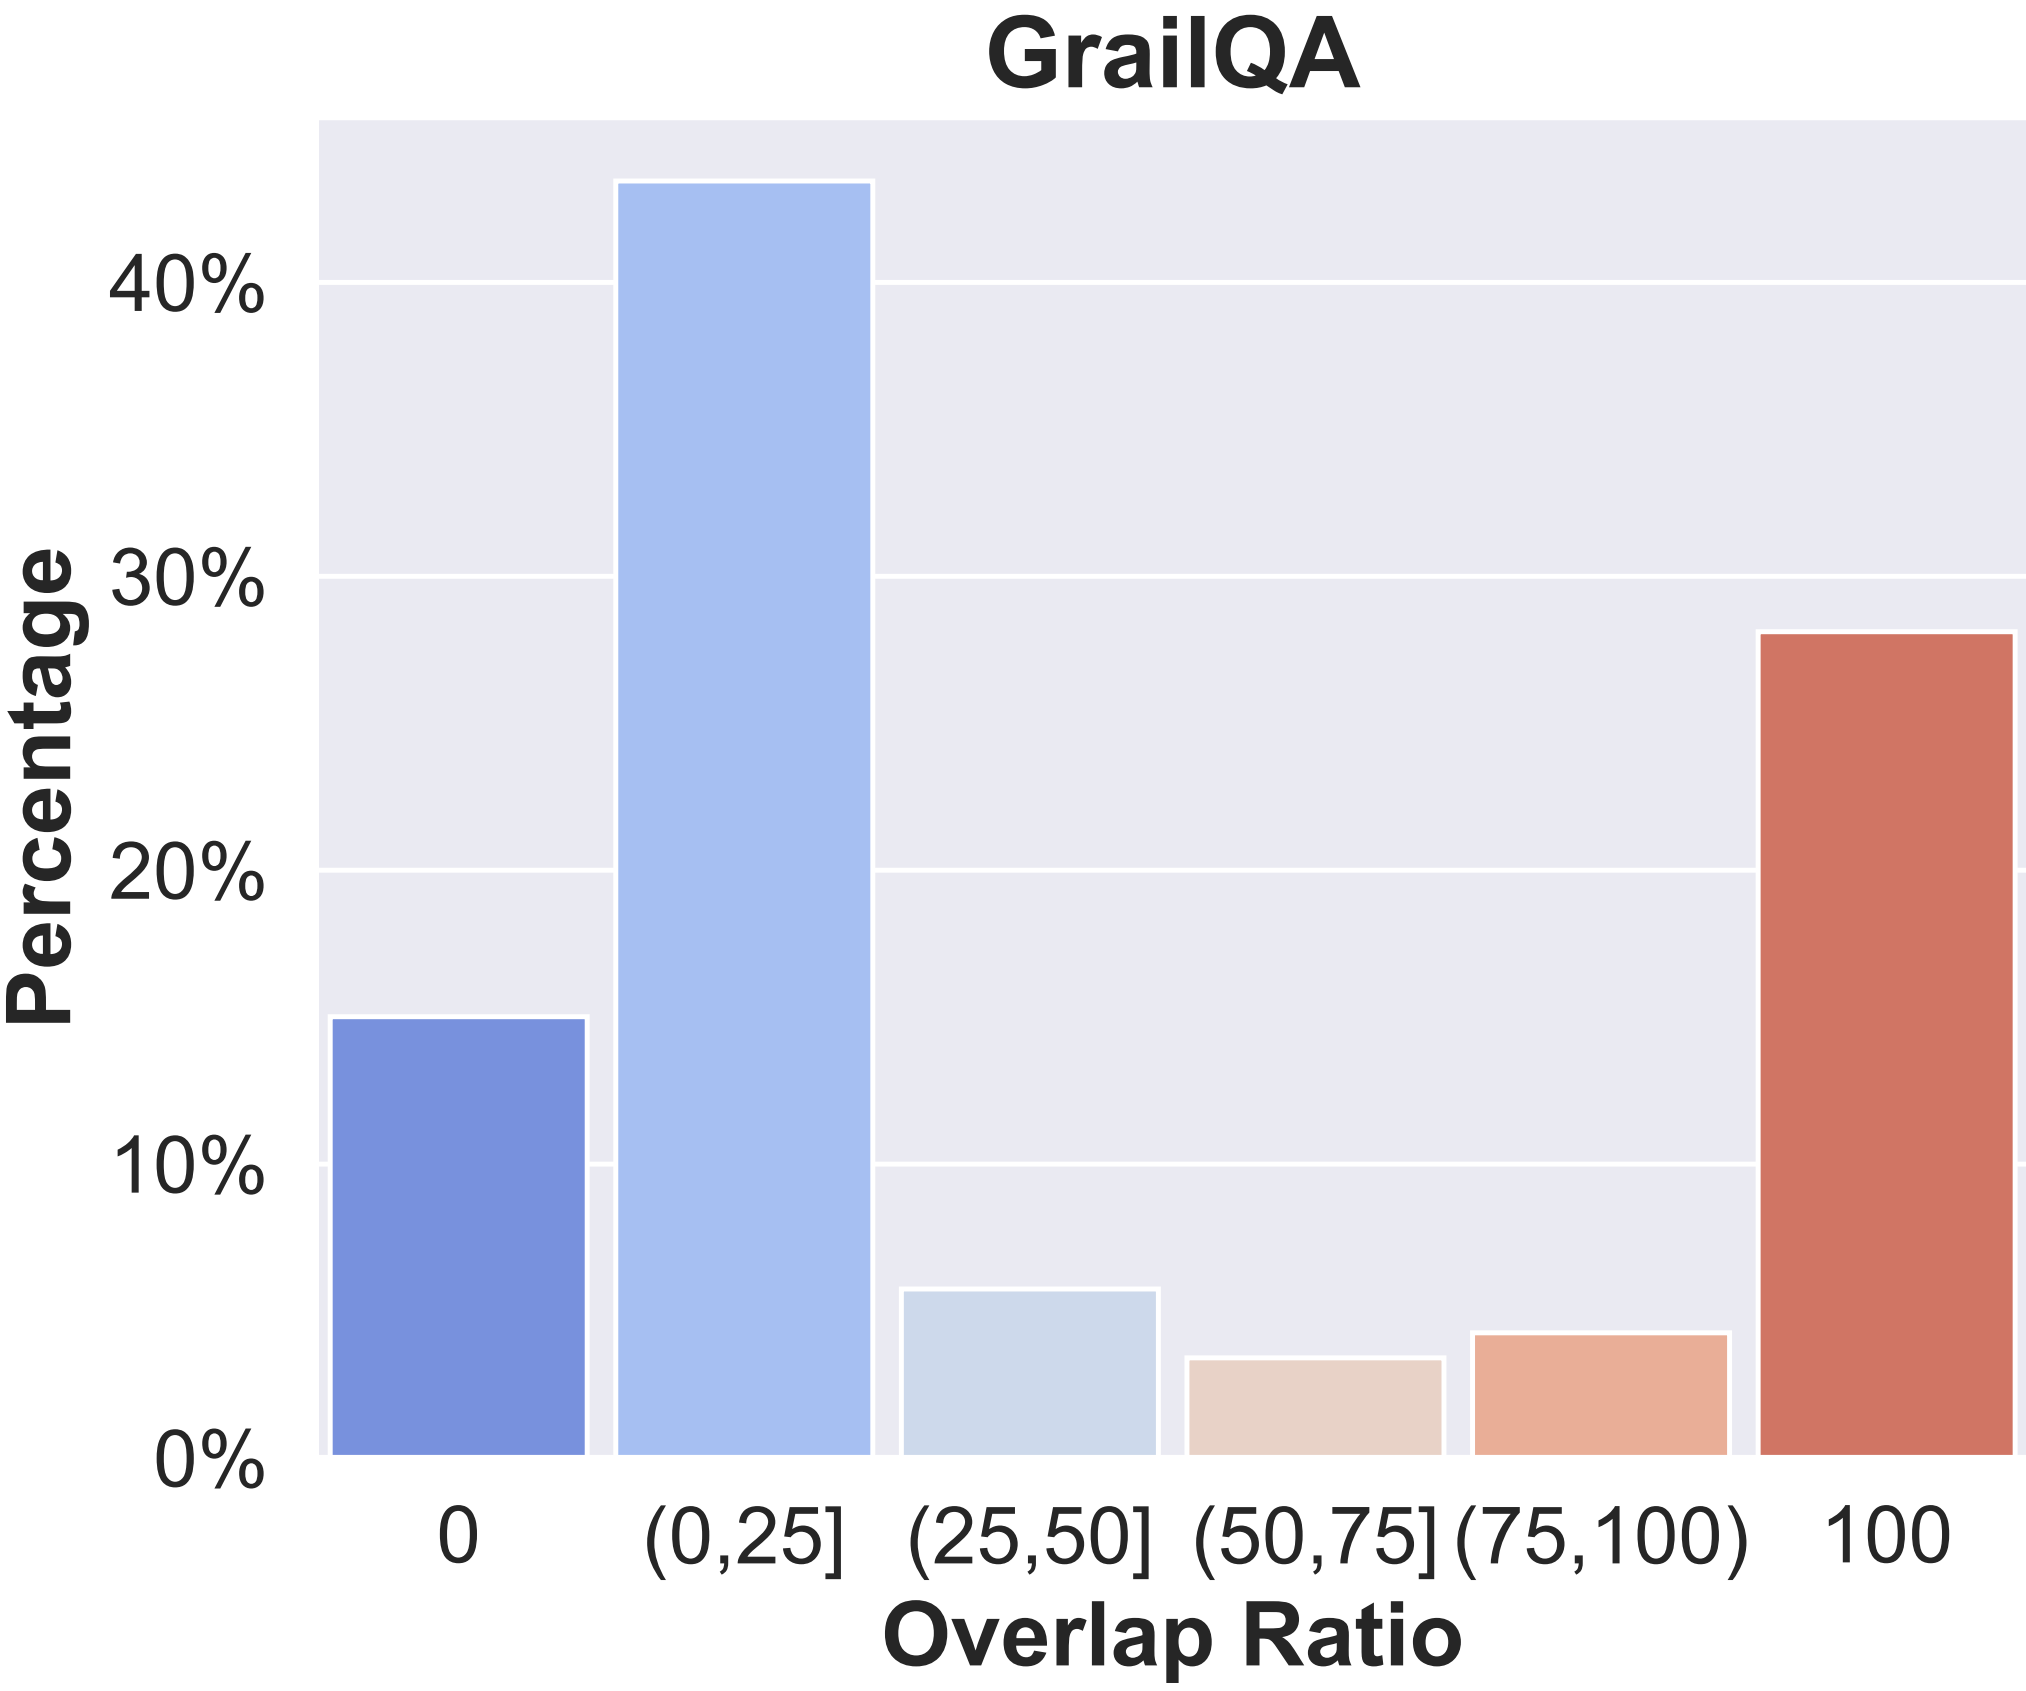
\includegraphics[width=\textwidth]{img/dis_grailqa.png}
    \end{subfigure}
    \caption{The explored path overlap ratio of ToG on CWQ, WebQSP, and GrailQA datasets.}
    \label{fig: overlap_ratio}
\end{figure}

\begin{figure}[htbp]
    \centering
    \begin{subfigure}[b]{0.32\textwidth}
        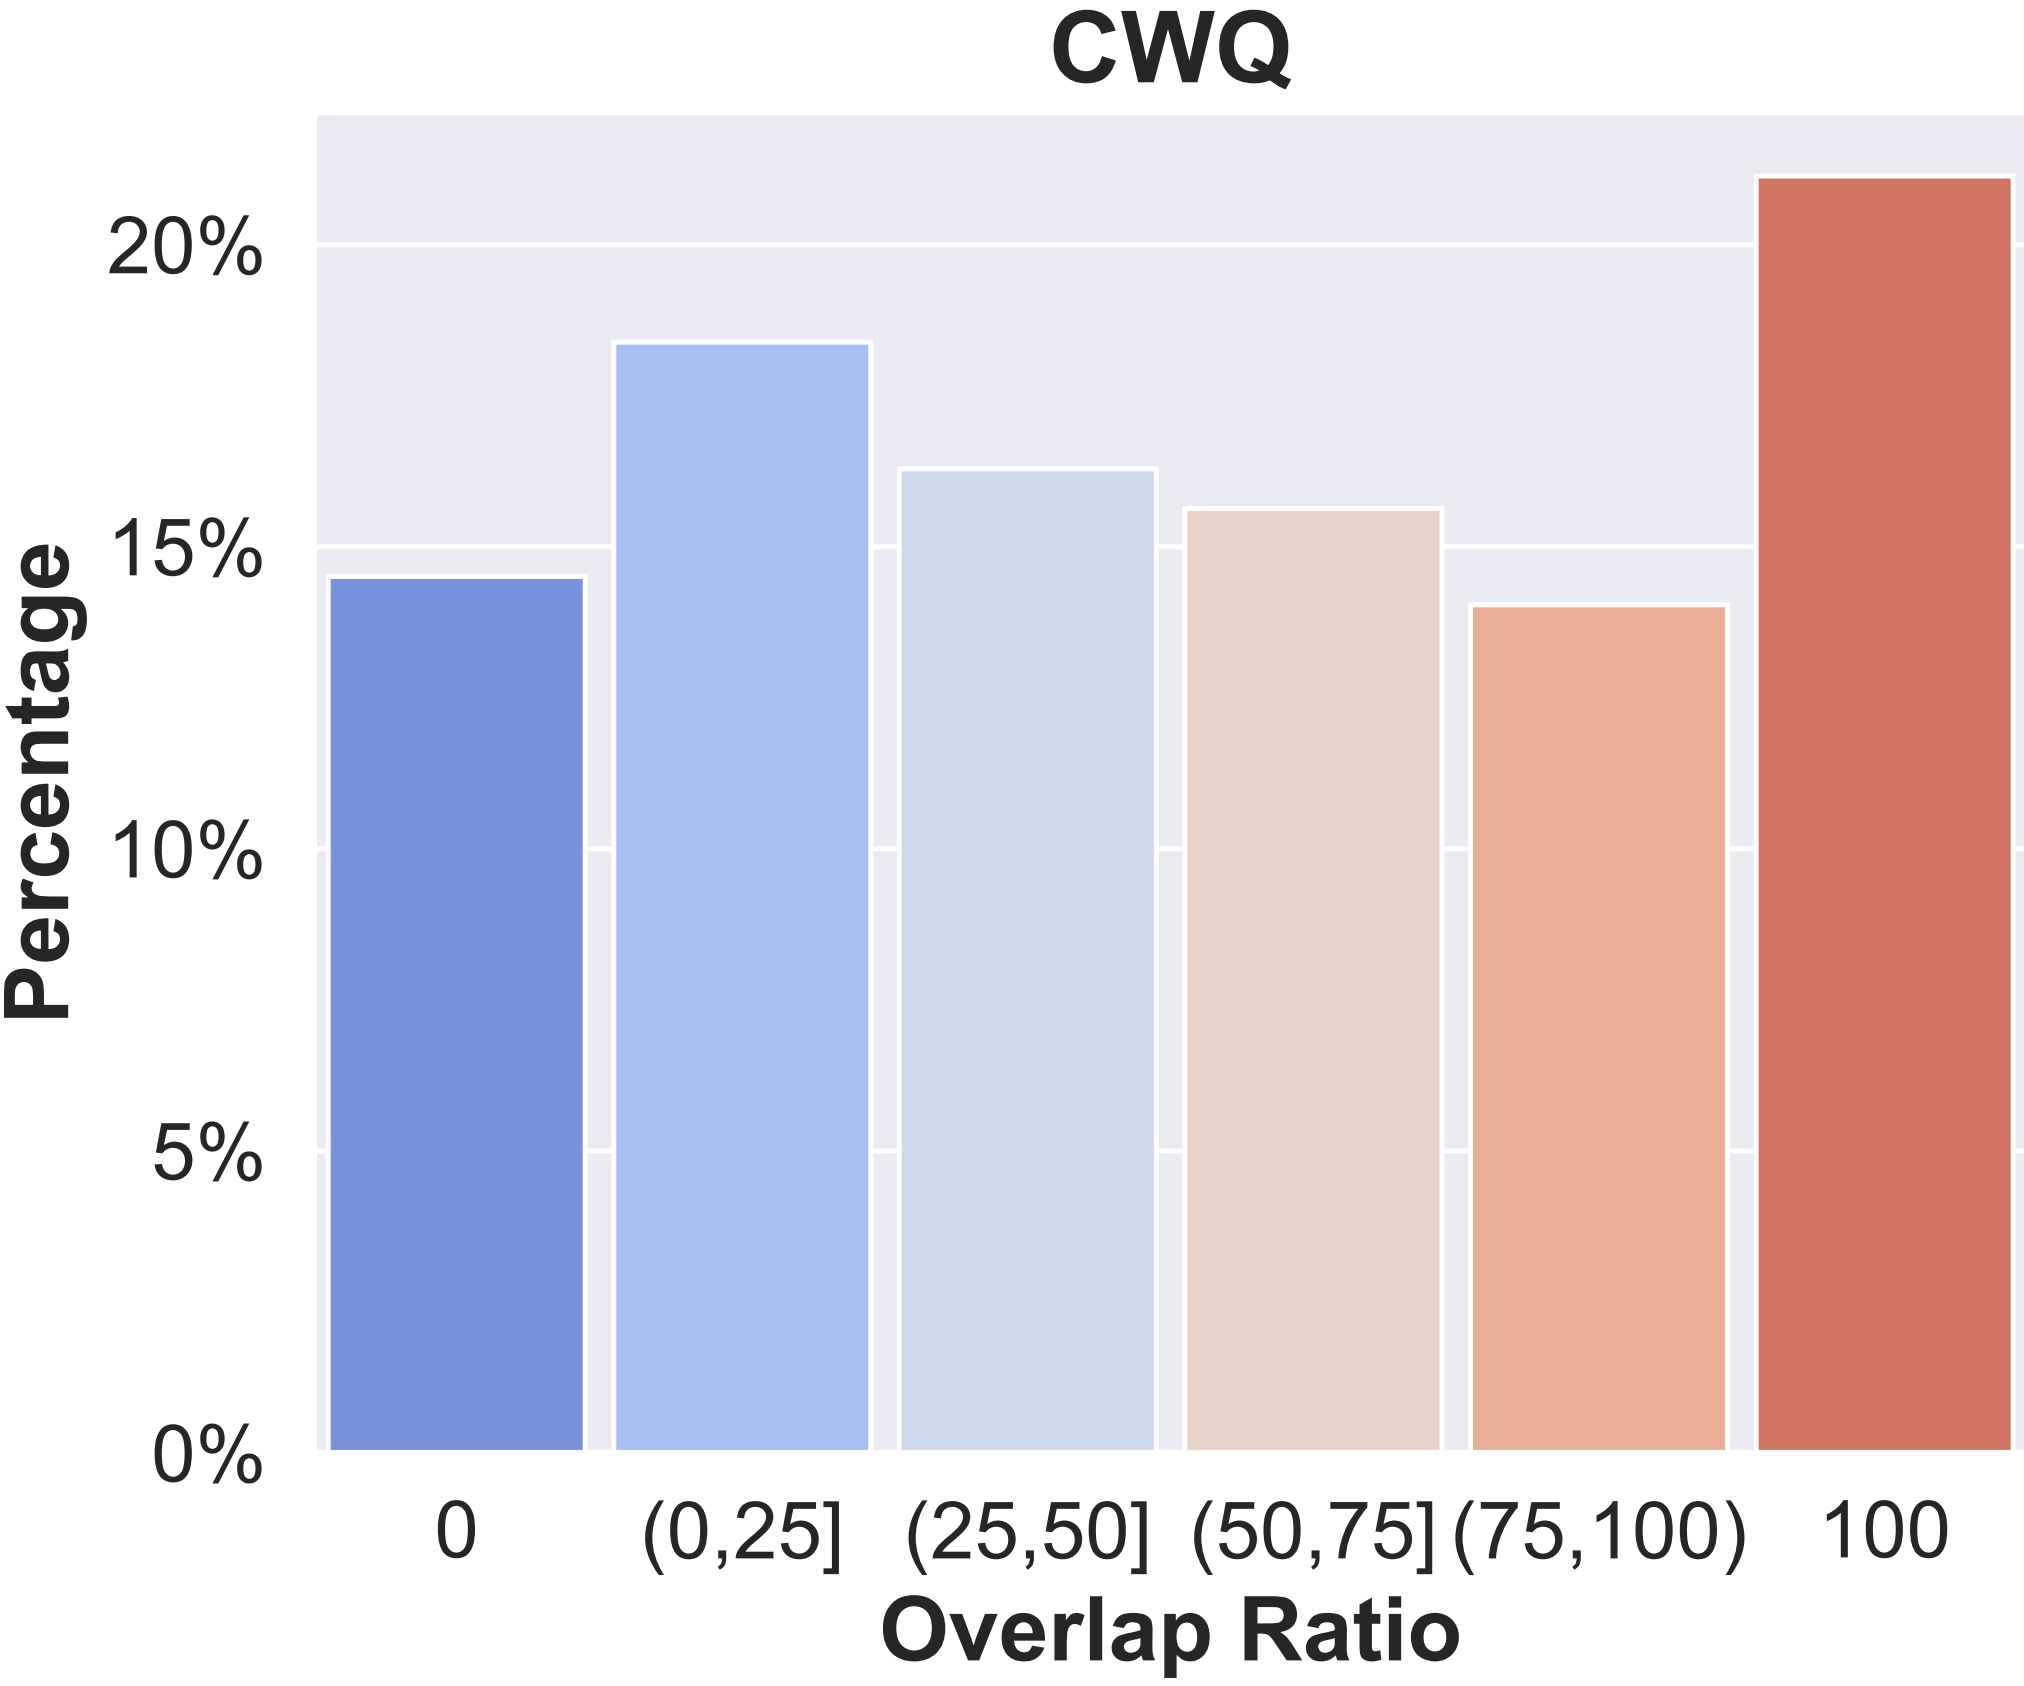
\includegraphics[width=\textwidth]{img/dis_cwq_togr.png}
    \end{subfigure}
    \hfill
    \begin{subfigure}[b]{0.32\textwidth}
        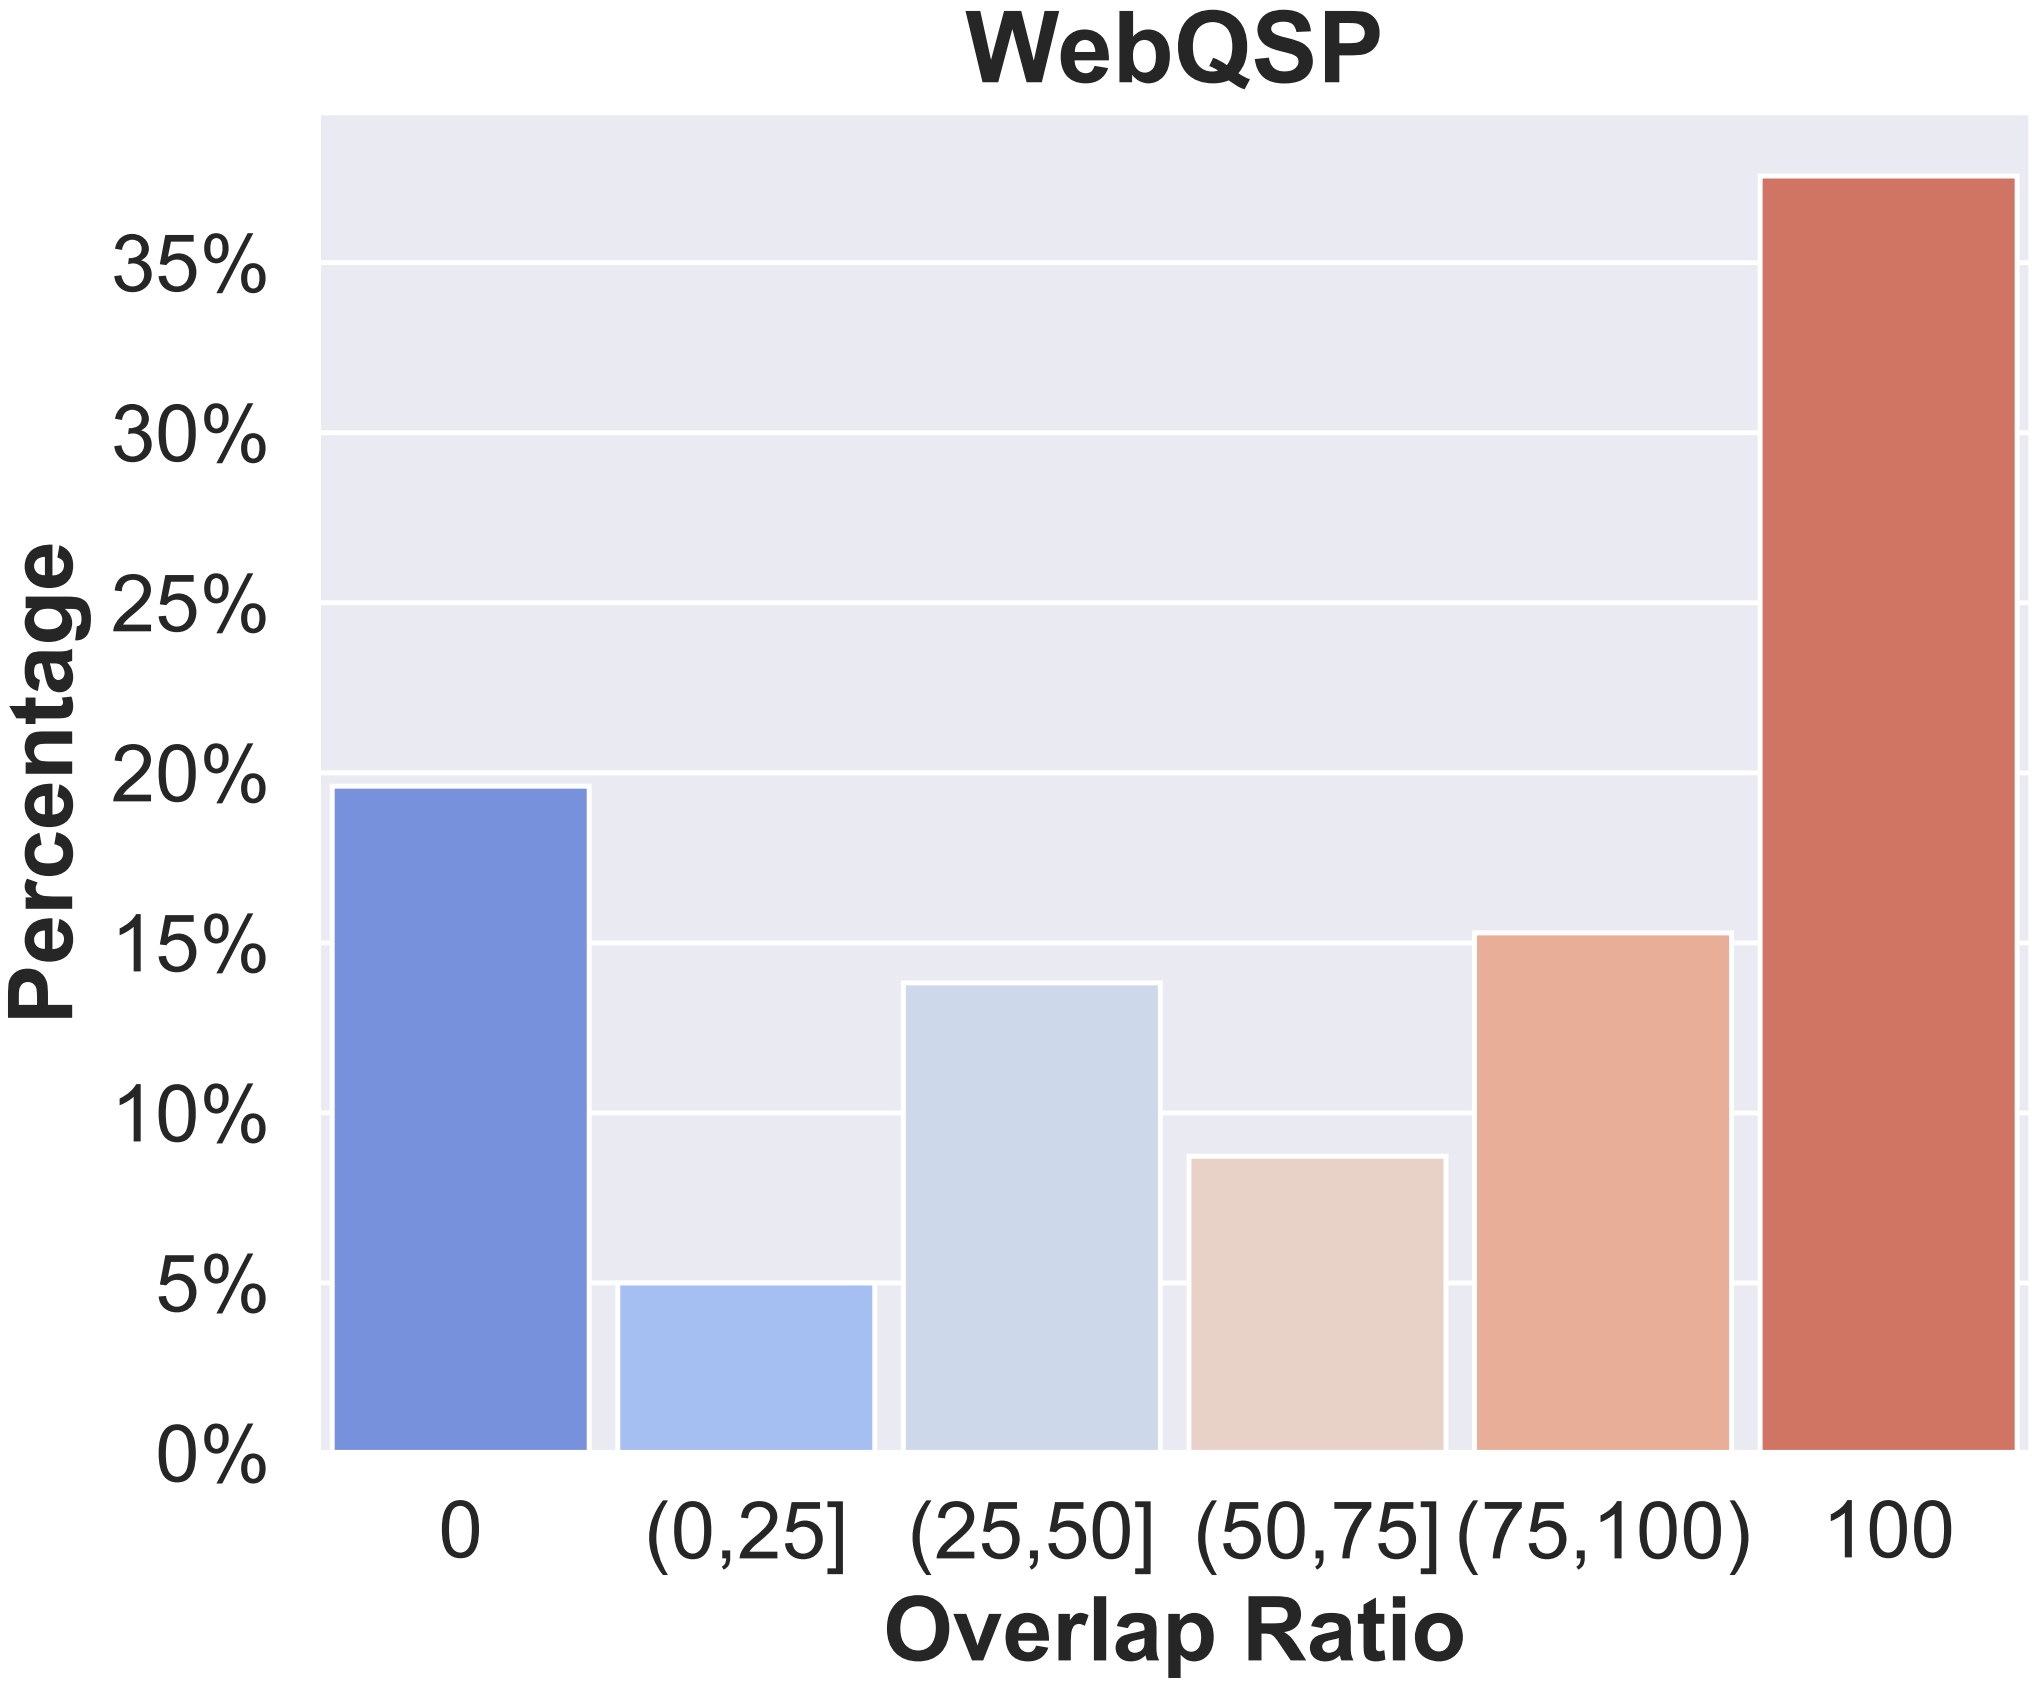
\includegraphics[width=\textwidth]{img/dis_webqsp_togr.png}
    \end{subfigure}
    \hfill
    \begin{subfigure}[b]{0.32\textwidth}
        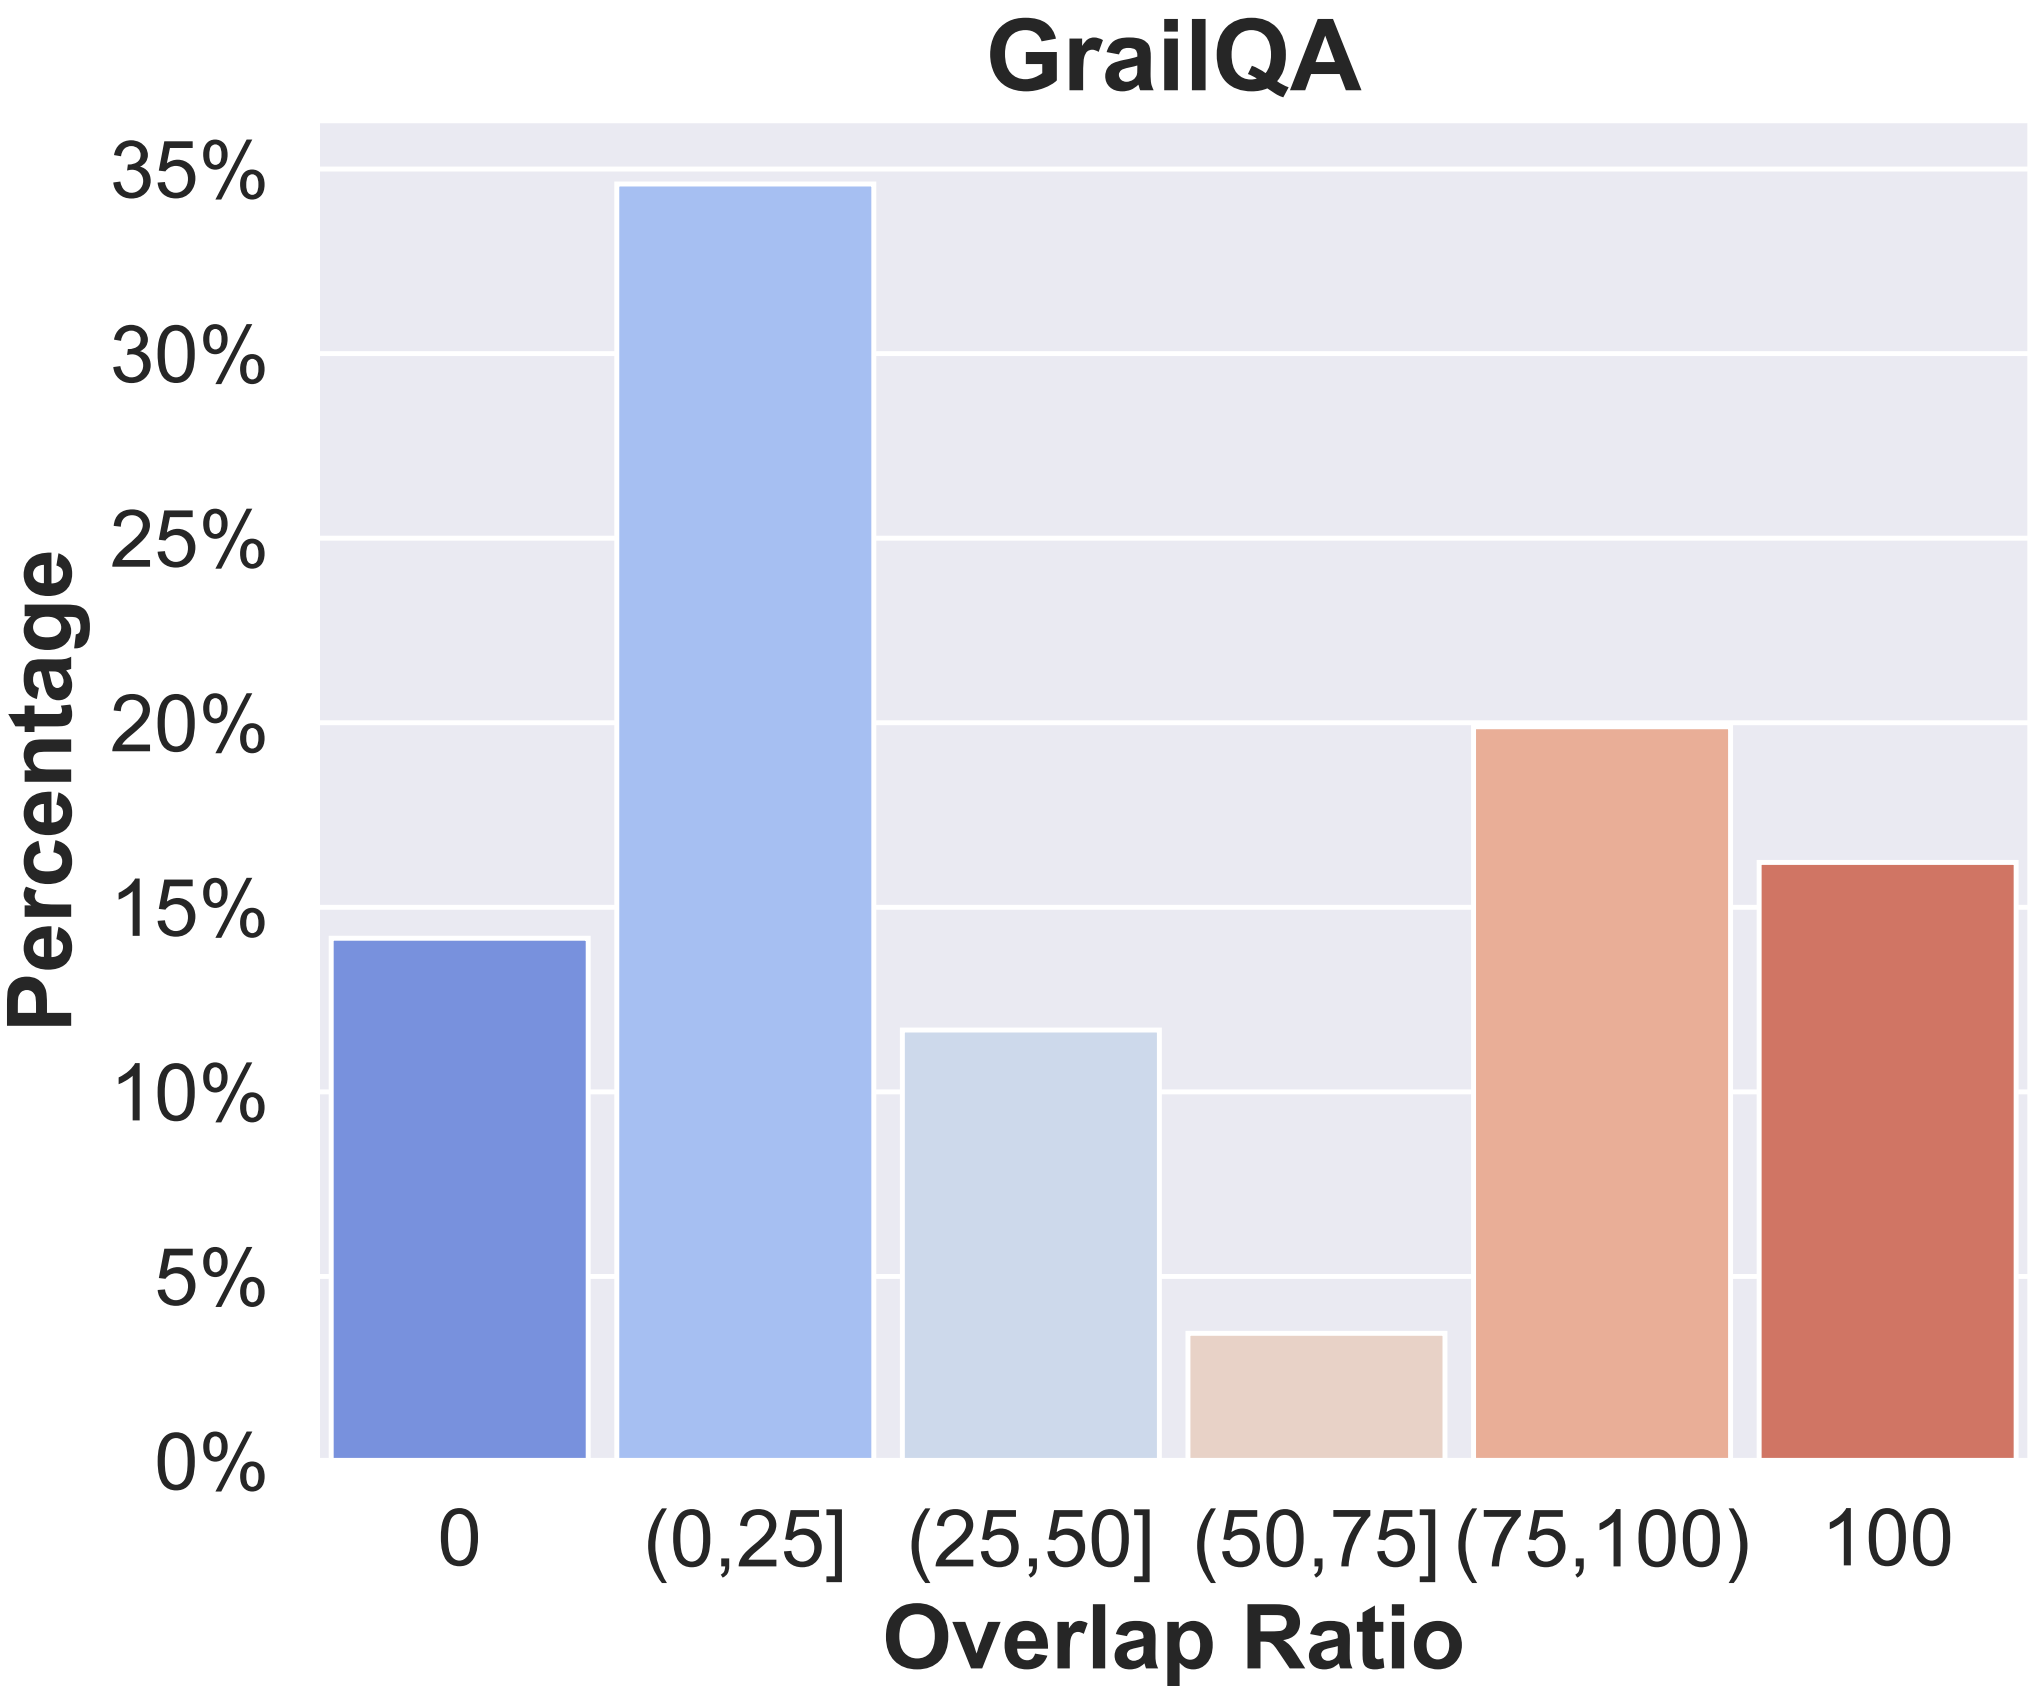
\includegraphics[width=\textwidth]{img/dis_grailqa_togr.png}
    \end{subfigure}
    \caption{The path overlap ratio of ToG-R on CWQ, WebQSP, and GrailQA datasets.}
    \label{fig: overlap_ratio_togr}
\end{figure}






\paragraph{The Reasoning Depth of Questions}

\begin{figure}
  \centering
  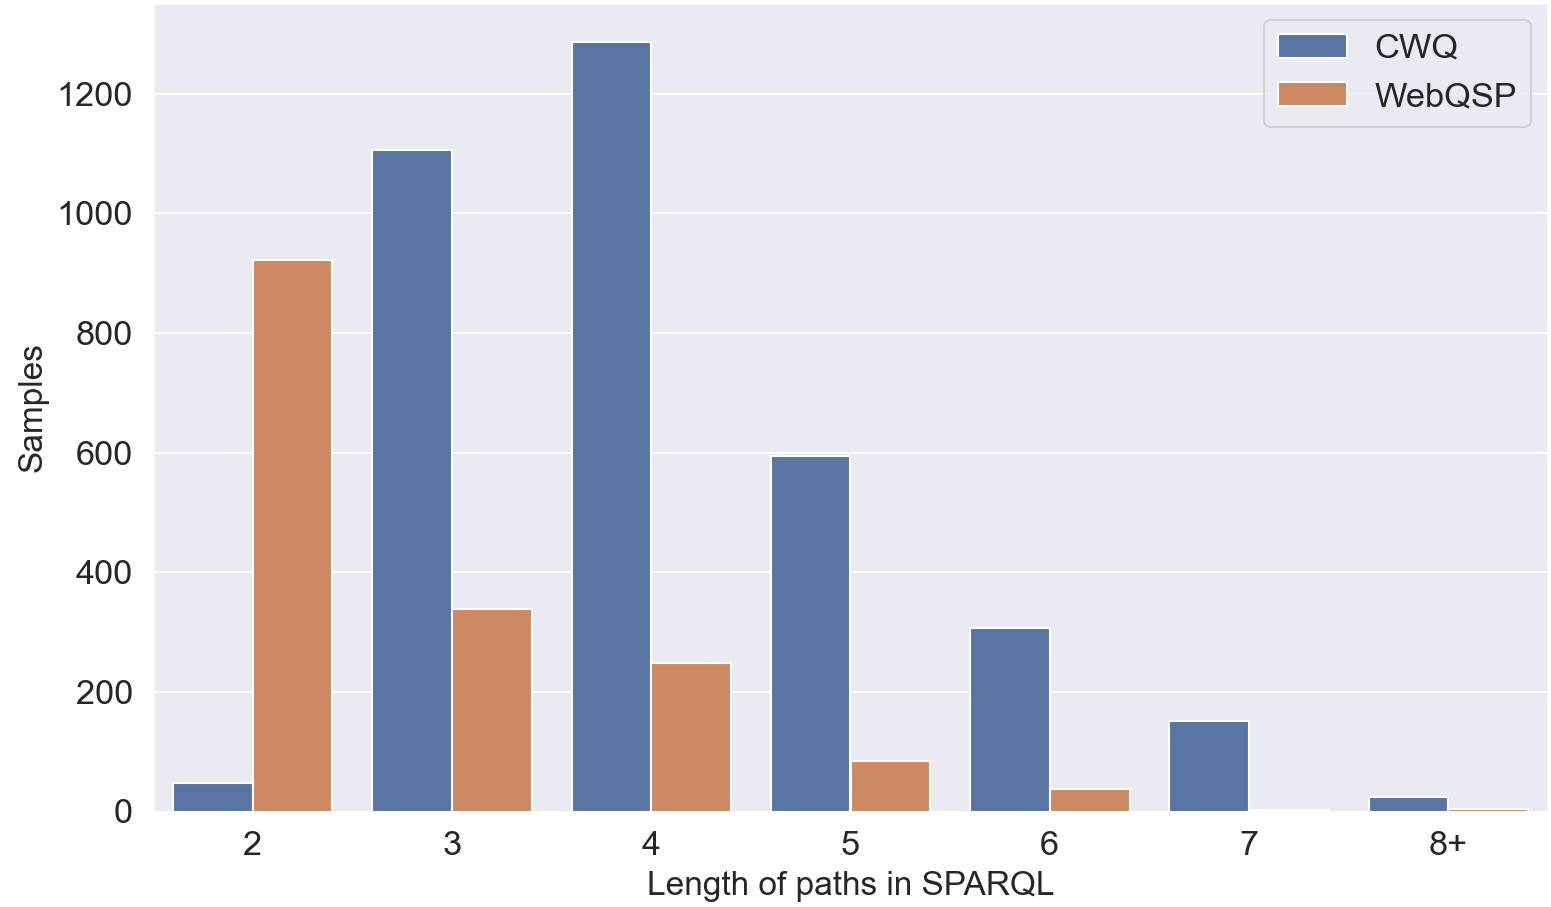
\includegraphics[width=0.7\textwidth]{img/cal_links.png}
  \caption{The lengths of the ground-truth SPARQL queries within the CWQ and WebQSP datasets, computed based on relation numbers.}
  \label{fig: cal_links}
\end{figure}

We calculate the reasoning depth of testing questions based on the number of relations within their ground-truth SPARQL queries on CWQ and WebQSP. The counts of questions with different reasoning depths are shown in Figure \ref{fig: cal_links}. We analyze the performances of ToG, ToG-R, and CoT on testing questions of both datasets with different reasoning depths. As illustrated in Figure~\ref{fig: right_proportion}, the performances of CoT show roughly decreasing trends on both datasets, with the reasoning depth of testing questions increasing. Conversely, ToG and ToG-R can partially counteract the performance degradation caused by the increment of reasoning depths of questions, especially on CWQ. Generally, the performance difference between ToG and CoT becomes more significant on deeper questions.
% It is evident that in comparison to WebQSP, CWQ samples require deeper reasoning (with only 1\% of questions answerable within 2 steps), rendering them relatively more challenging inquiries. We perceive that deeper questions possess greater levels of complexity, and the inclusion of three-step reasoning in ToG successfully addresses approximately 60\% of the challenges presented in CWQ, approaching nearly state-of-the-art performance.

% \subsection{Path Schematic}
% We describe the methods we calculate the overlap of paths in Section \ref{fig: overlap_ratio}, and here is a specific path schematic (we use Table \ref{table: case4} for example).

% % 链路示意图+几句话描述，图的label要为fig: 
% \ref{fig: path_schematic} describes the difference between our link and the ground truth link. Many times ToG will explore a path that is slightly different from ground truth, but both paths lead to the correct answer

\begin{figure}[t]
    \centering
    \begin{subfigure}[b]{0.44\textwidth}
        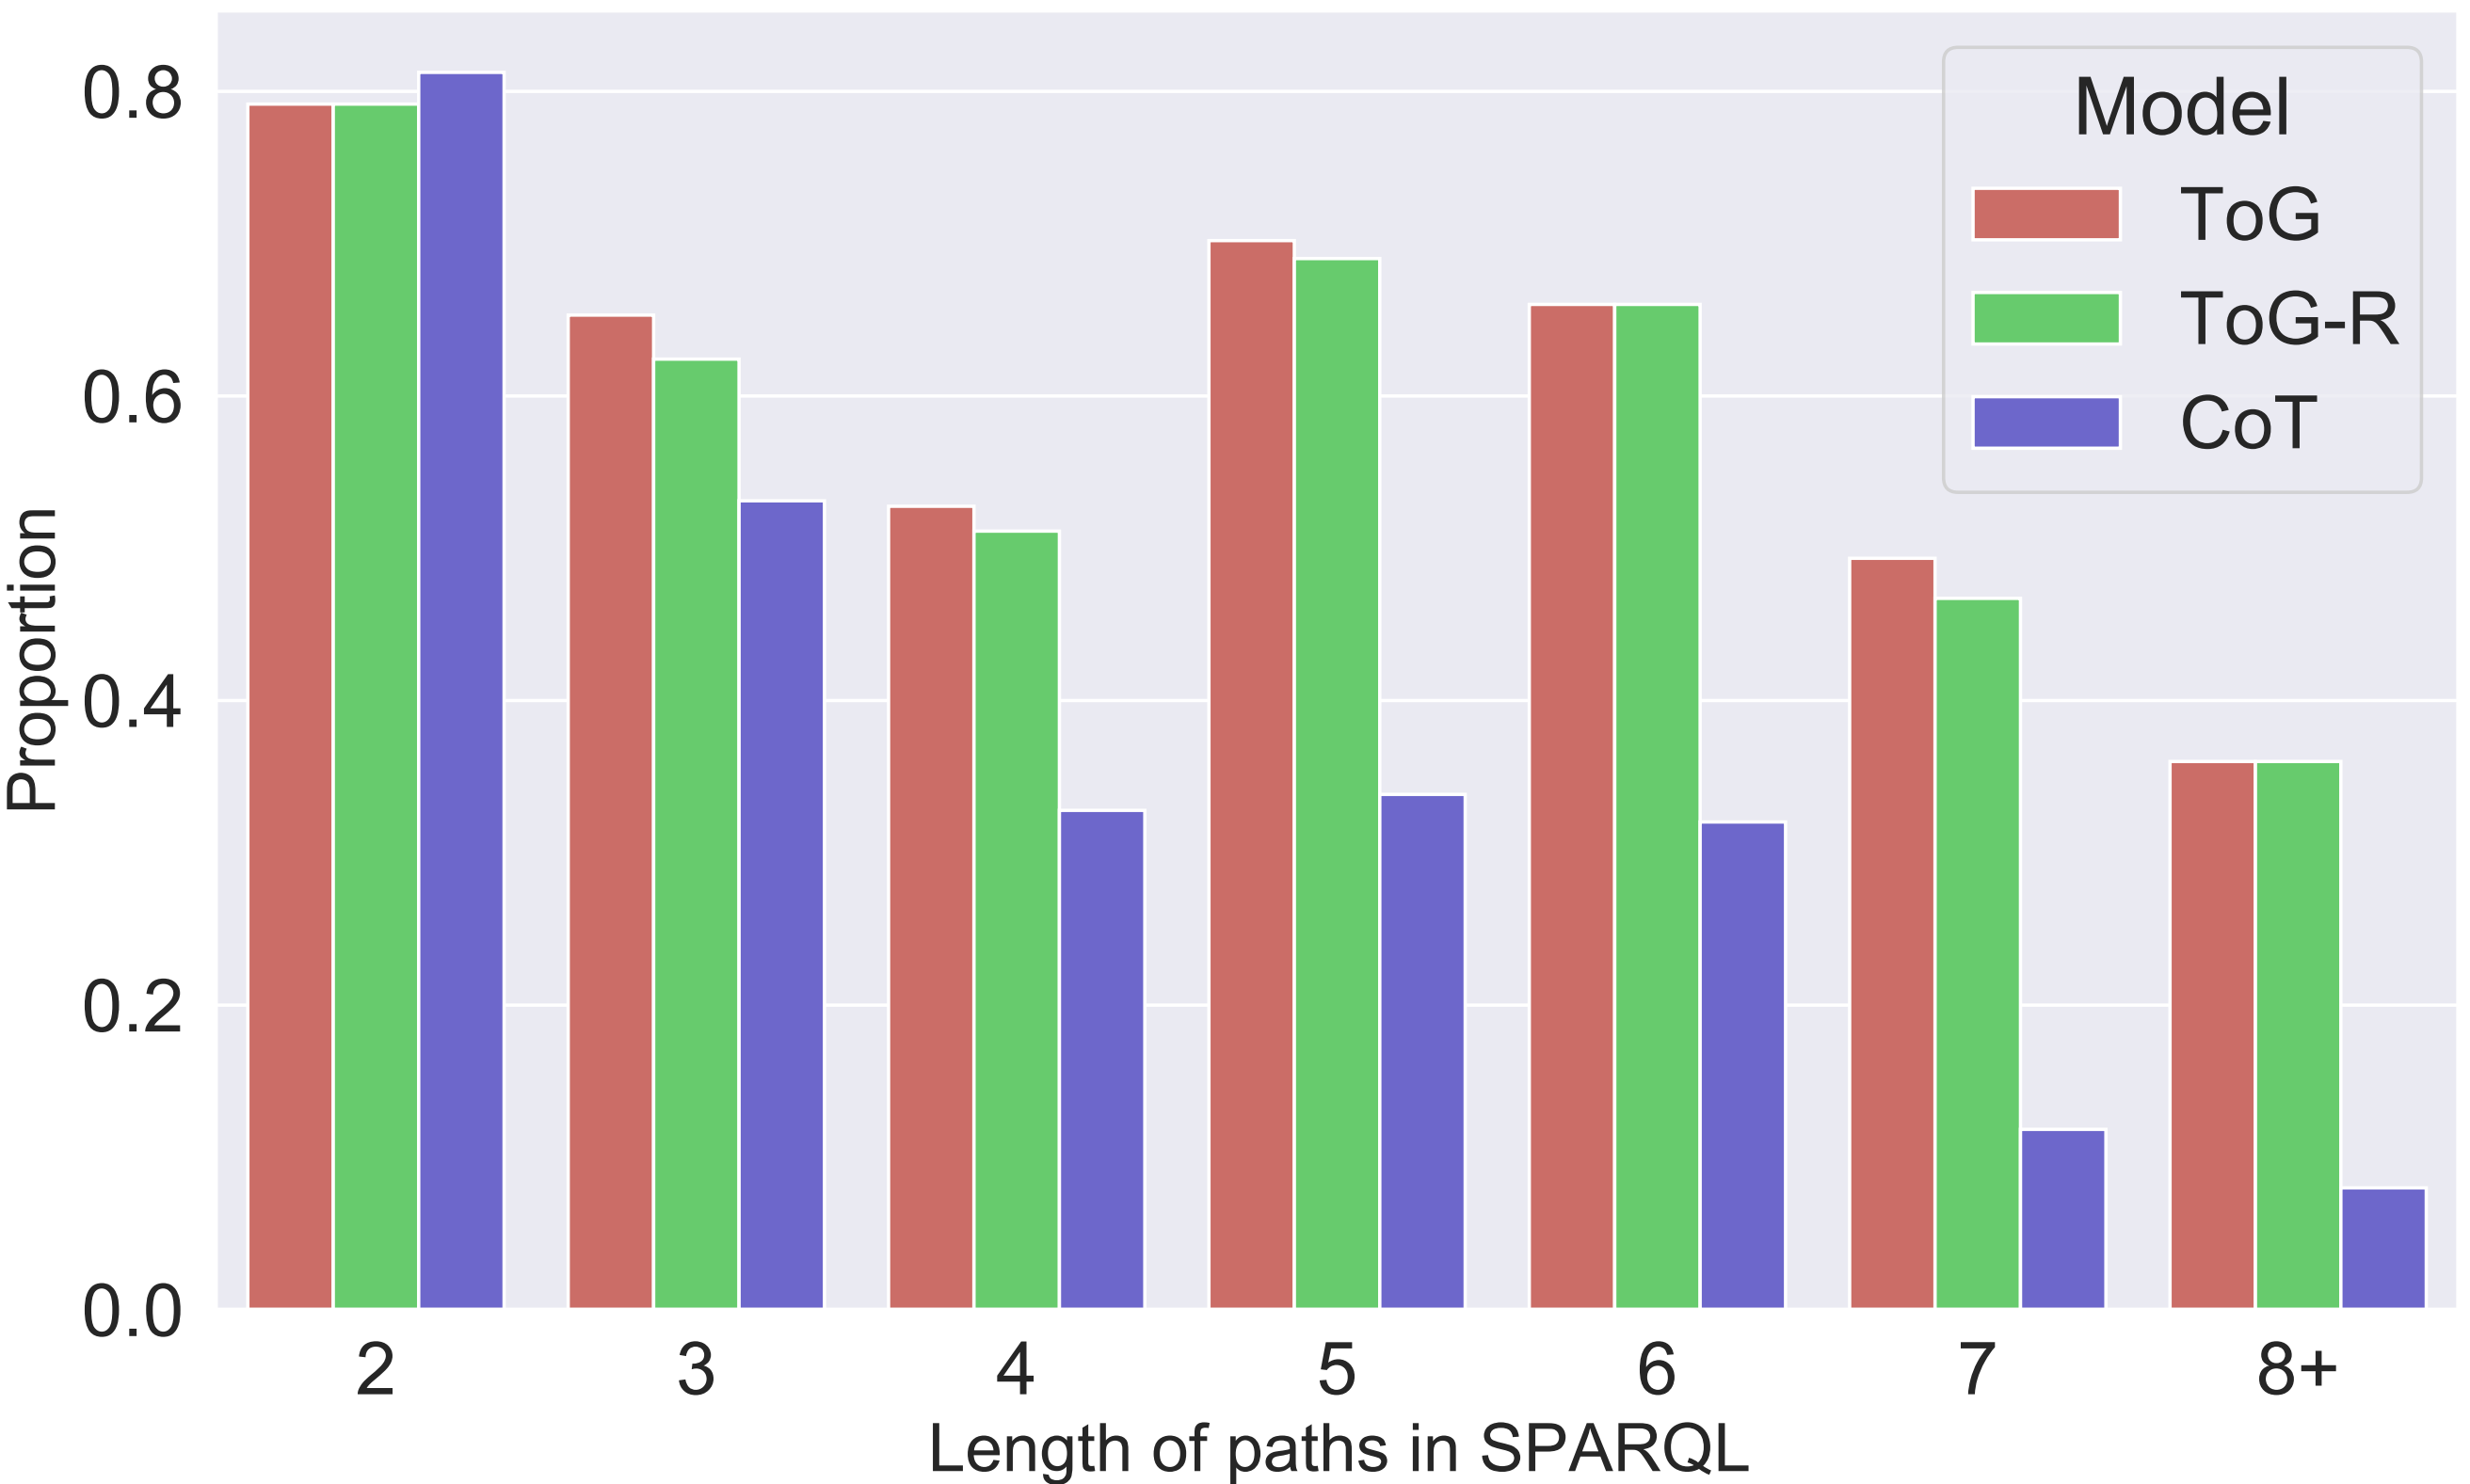
\includegraphics[width=\textwidth]{img/model_performance_cwq.png}
    \end{subfigure}
    % \hfill
    \begin{subfigure}[b]{0.44\textwidth}
        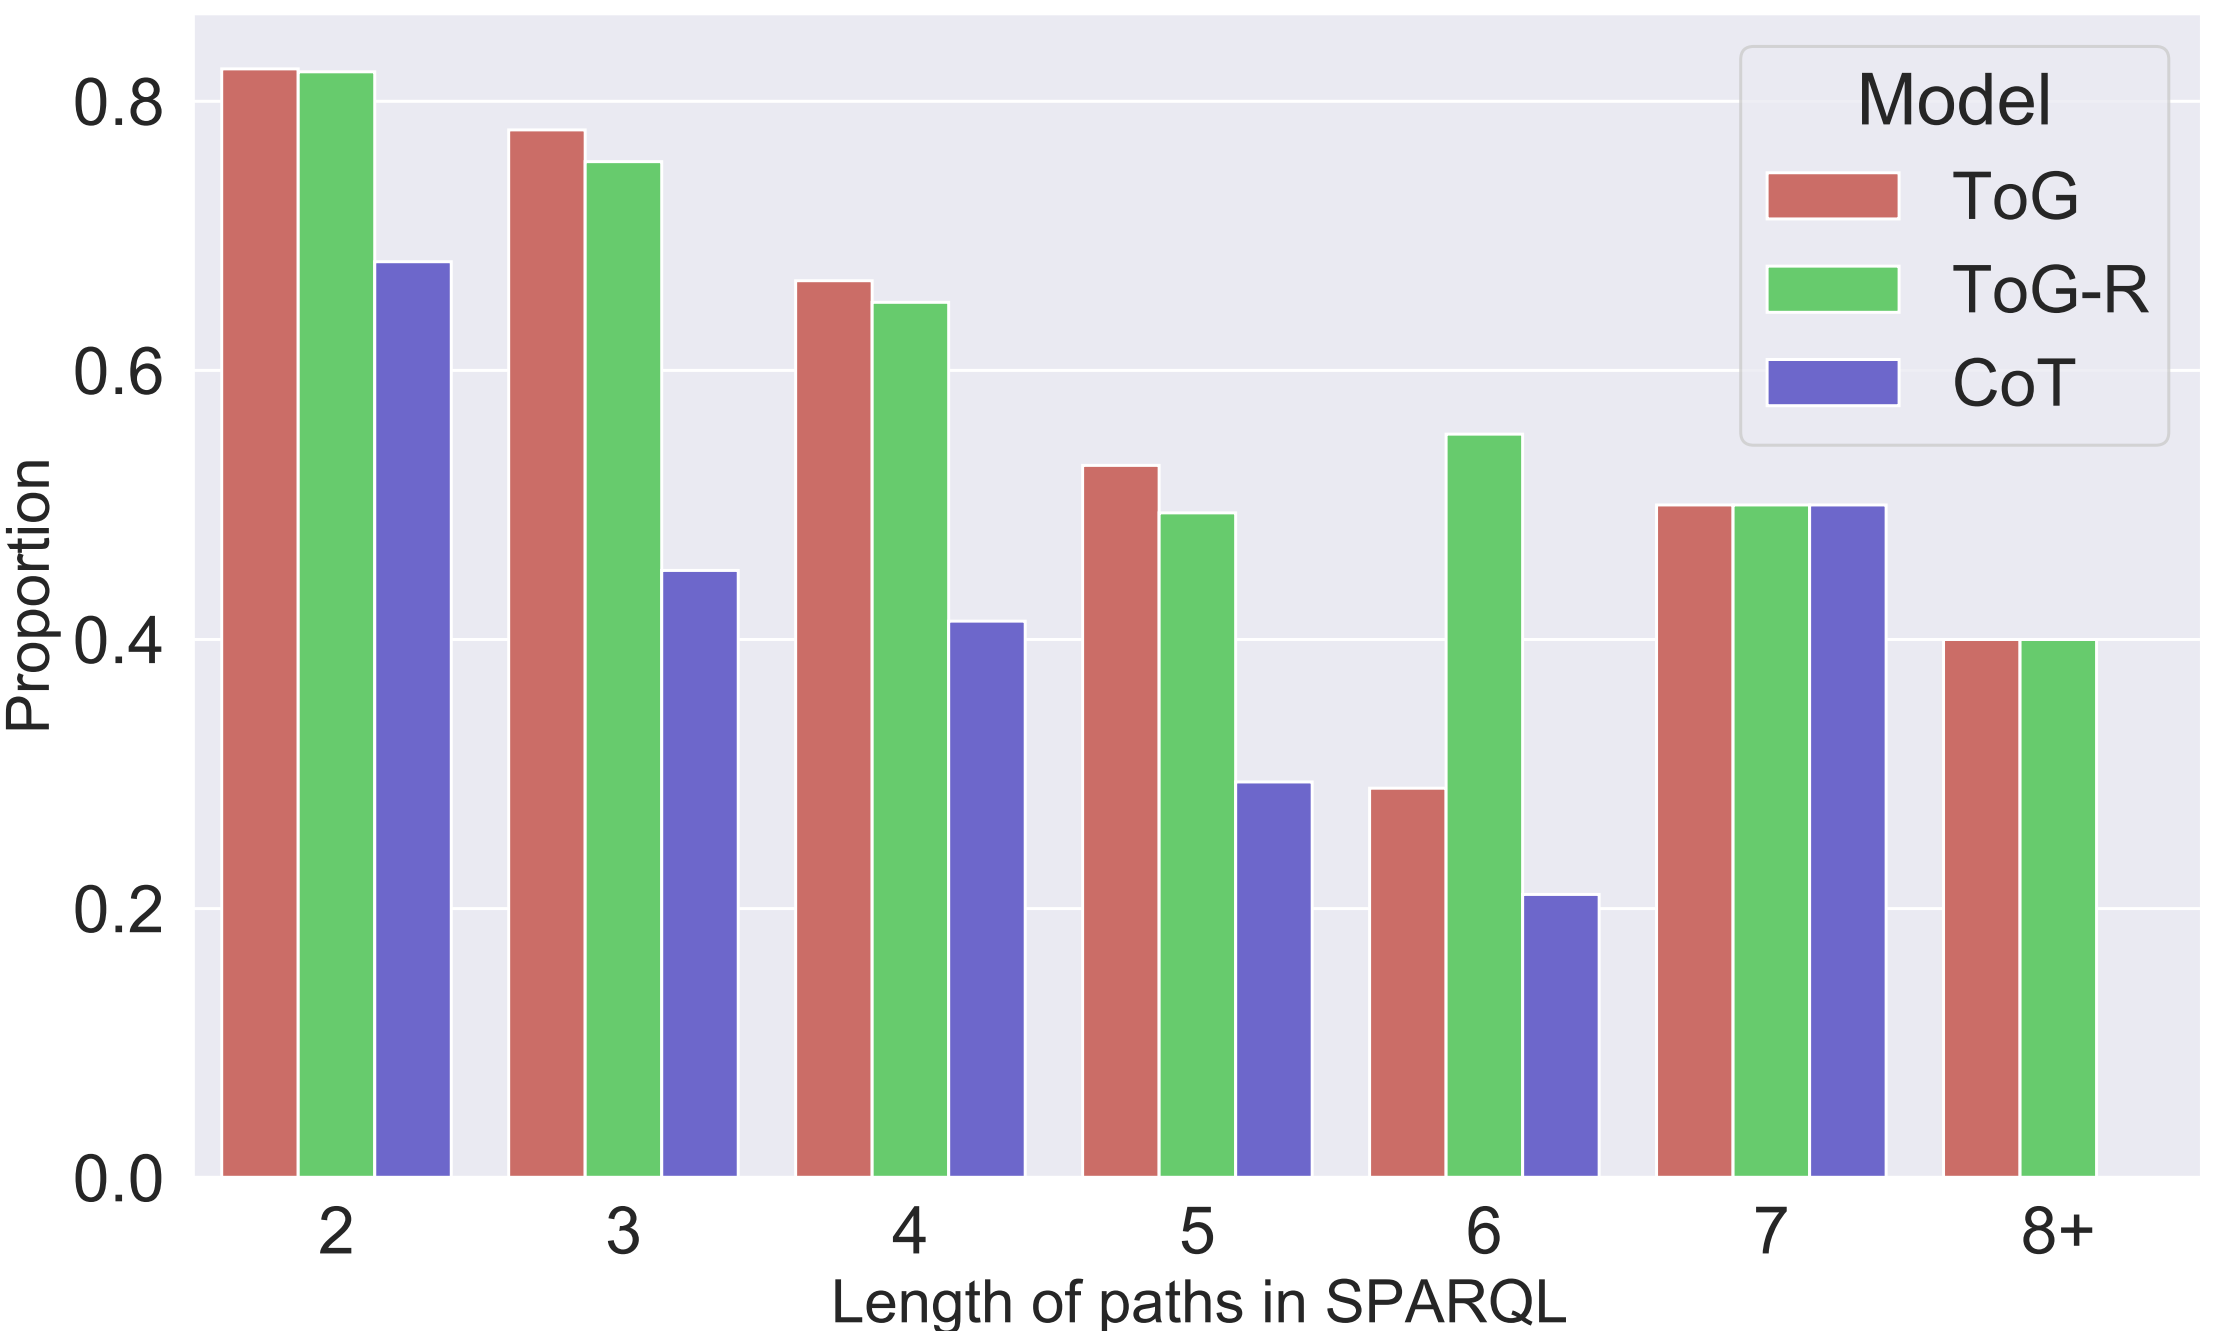
\includegraphics[width=\textwidth]{img/model_performance_webqsp.png}
    \end{subfigure}
    \caption{ToG, ToG-R and CoT's performance among CWQ and WebQSP dataset.}
    \label{fig: right_proportion}
\end{figure}

% \begin{figure}[htbp]
%     \centering
%     \begin{subfigure}[b]{0.49\textwidth}
%         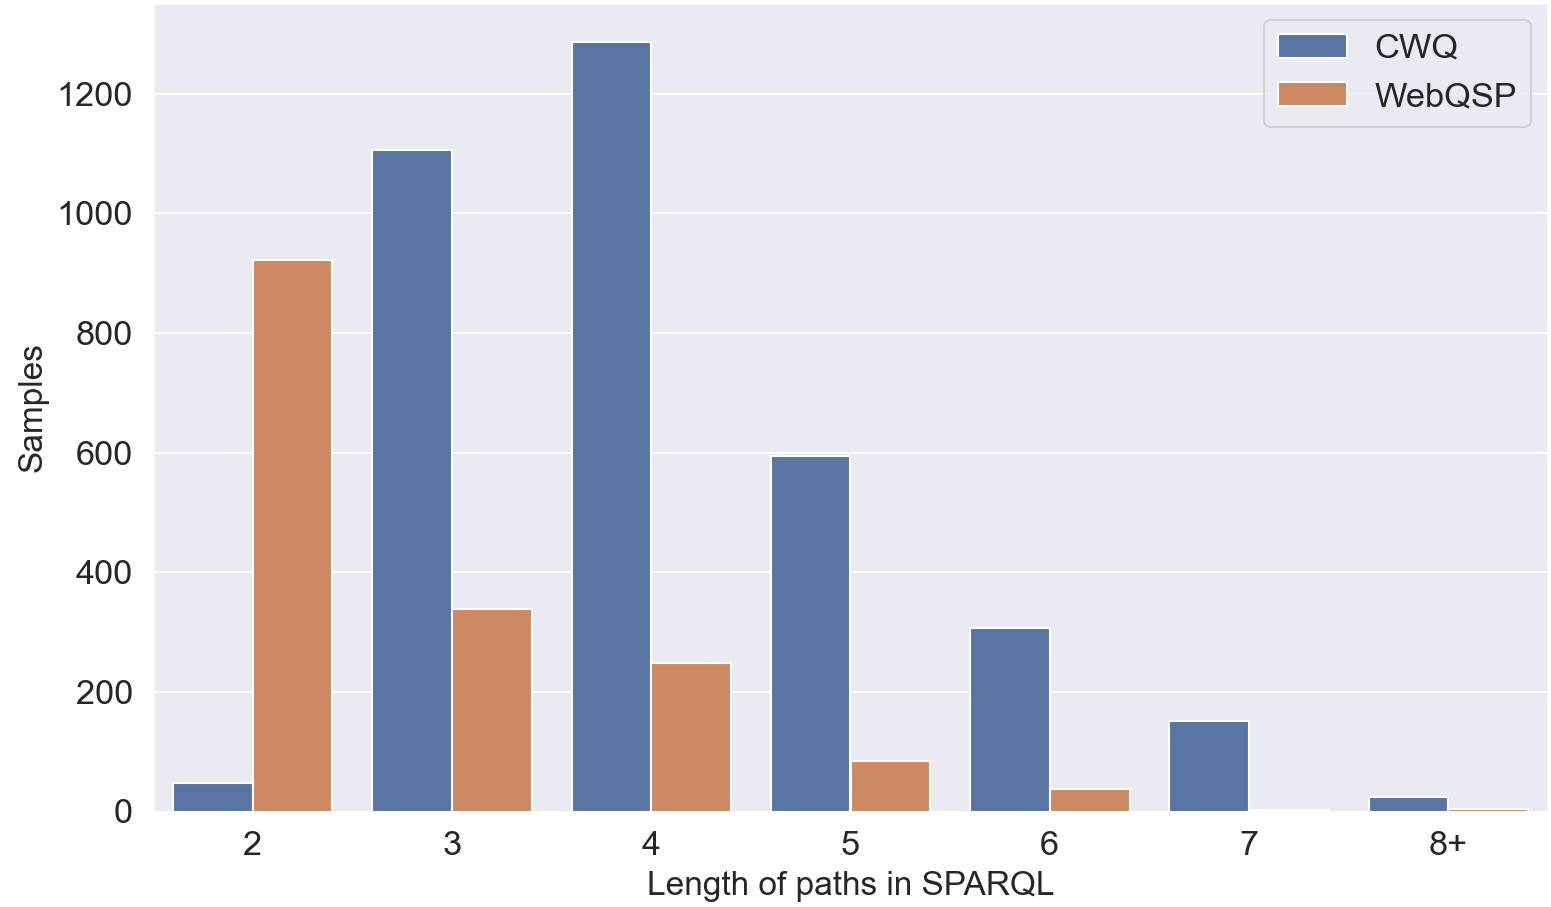
\includegraphics[width=\textwidth]{img/cal_links.png}
%     \end{subfigure}
%     \hfill
%     \begin{subfigure}[b]{0.49\textwidth}
%         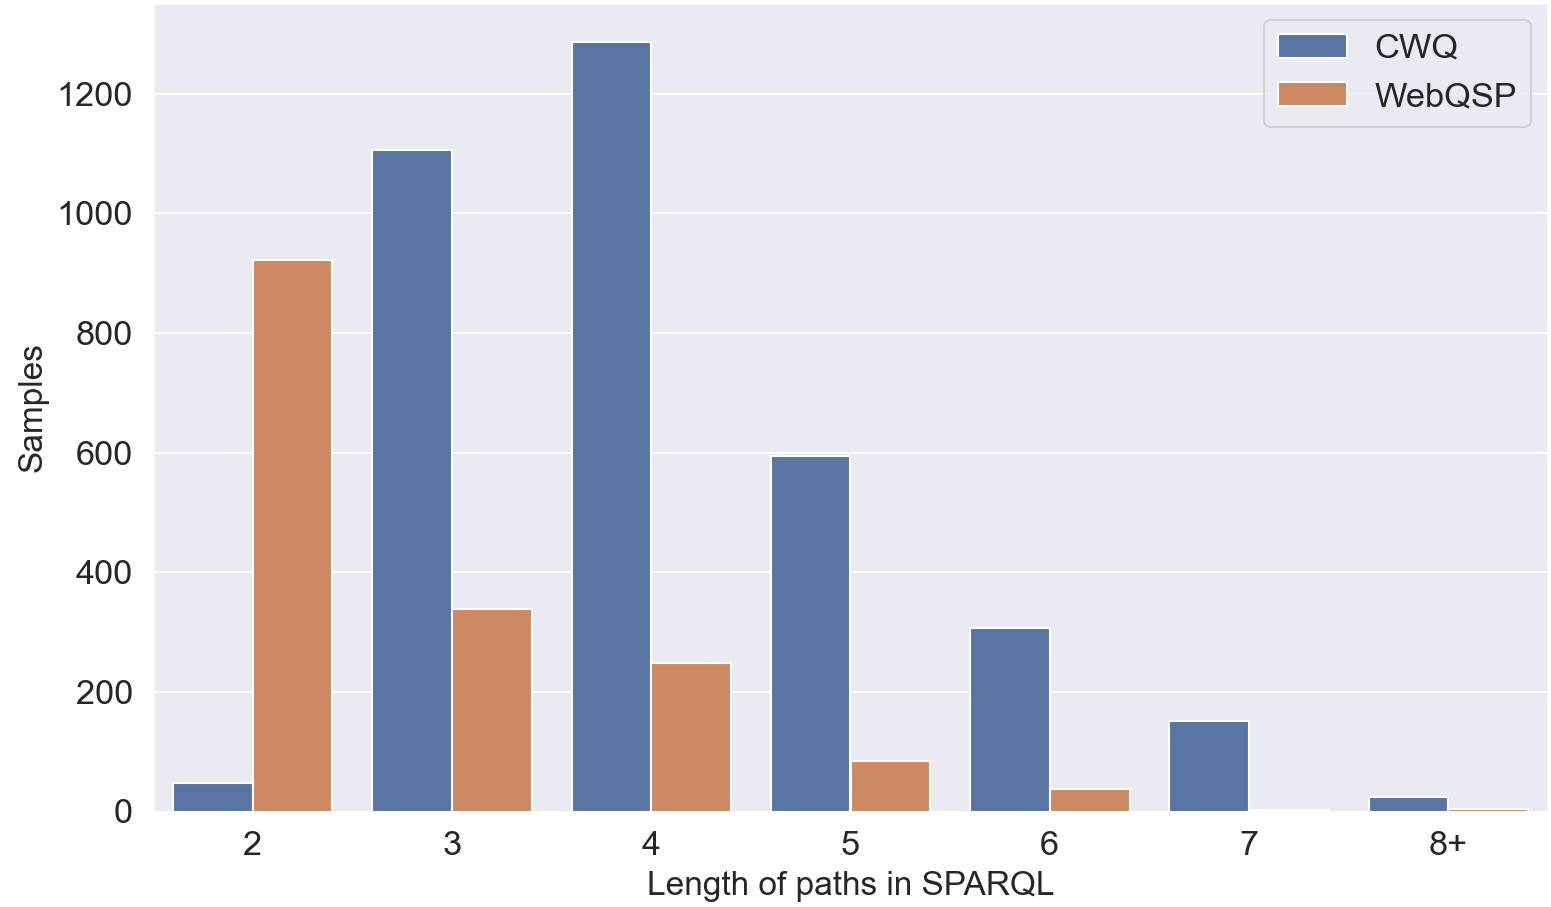
\includegraphics[width=\textwidth]{img/cal_links.png}
%     \end{subfigure}
%     \caption{The lengths of the ground-truth SPARQL queries within the CWQ and WebQSP datasets, computed based on relations.}
%     \label{fig: cal_links}
% \end{figure}

\subsubsection{Efficiency of ToG}
There are many solutions to improve efficiency and reduce the computational complexity (proportional to the number of calling LLMs) of ToG from the original $O(ND)$ to $O(D)$, where $D$ is the depth (or equivalently length) of the reasoning path, and $N$ is the width of the beam-search (how many paths are remained in the pool in each iteration).

\paragraph{Solution 1}
Reducing computational complexity from $O(ND)$ to $O(D)$ by using lightweight model in pruning. The bottleneck of computation is the pruning step, which contributes to $N*D$ times calling, and it is important to optimize it for computational efficiency. A technical route is to replace LLM with small models such as BM25 and Sentence-BERT in the pruning step since the small models are much faster than LLM calling. In this way, we can reduce the number of LLM calling from $2ND+D+1$ to $D+1$. When $D$=3, for example, there are only 4 times LLM calling. However, this optimization sacrifices the accuracy due to the weaker scoring model in pruning. For instance, as shown in Table \ref{table: tools} of the manuscript, the performance of ToG on WebQSP drops from 76.2\% to 66.3\% after replacing ChatGPT with SentenceBERT for pruning. To alleviate the issue of the performance degradation, we can appropriately increase the search width to compensate the loss because increasing search width can improve the chance of the optimal path to be selected in the pool and it doesn't affect the number of LLM calling. To empirically verify this, we increase the search width from 3 to 5 and reevaluate ToG with SentenceBERT as the pruning model on WebQSP. The accuracy rises to from 66.3\% to 68.5\% and could be further improved with a greater width since the greater width would not cause an increase in the number of LLM calls.

\paragraph{Solution 2}
Reducing computational complexity from $O(ND)$ to $O(D)$ by unifying the prompts in the same pruning step. Another solution on speeding up the pruning step is to employ the LLM at once to score all components of N candidate sets for obtaining top-N candidates, instead of calling the LLM N times to score N candidate sets separately. Through this solution, either entity pruning step or relation pruning step only need 1 LLM call for each iteration. Thus, the maximum number of LLM calls per question needed for ToG and ToG-R would drop to $2D+D+1$ and $D+D+1$.

\paragraph{Solution 3}
Optimizing pruning step to make the actual calls of LLMs much less than the previously estimated $2ND+D+1$ and closer to some common prompting methods such as CoT-SC. For ToG and other LLM-based methods, the computational time (cost or complexity) in the inference phase mainly depends on how many times calling LLM. For each question, ToG needs at most $2ND + D + 1$ times. Meanwhile, ToG-R needs at most $ND+D+1$ times as mentioned in Section \ref{sec: methods}. 

Given the beam search width $N$ and maximal reasoning depth $D$, ToG's initialize the search from the entity mostly aligning with the keyword in question. In each iterative step of the reasoning path, ToG starts from each of the $N$ entities/relations (nodes/edges on knowledge graph) and searches all its neighboring relations/entities. Given the search width $N$, ToG always keep $N$ "most-likely" candidate reasoning paths in the pool, and thus there are always $N$ candidate entity sets $E^D_{cand,n}$ and $N$ candidate relation sets $R^D_{cand,n}$. Consequently, it needs $N$ LLM calls for entity pruning and $N$ calls for relation pruning, respectively, as well as one additional LLM call for reasoning (evaluating if the information from the current candidate paths are enough or not). We have to point it out that, for each of the $N$ starting entities, all its neighbor entities/relations are NOT scored one by one. On the contrary, all its neighbor entities/relations are "translated" into "one" prompt altogether and are sent to LLM, which output the top-$N$ candidates at one-time. Therefore, each starting entity only calls LLM once for pruning and so $N$ starting entities calls LLM $N$ times in one iterative step. Consequently, there are totally $2ND+D$ times calling after reasoning $D$ steps. In the end, there is an additional calling that "translate" the final path to user-understandable language and answer the user. Therefore, ToG requires $2ND+D+1$ LLM calls in total. Since most questions can be answered within 3 hops (means depth of reasoning path is 3), and the performance is usually good enough when the search width $N$=3 as we tested in Figure \ref{fig: depth_width}, the total number of LLM calling is $2\times 3\times 3+3+1=22$. So the computational time is about 21 times longer than that of LLM-only. With a similar performance to ToG, its variant ToG-R only calls LLM for $ND+D+1$ times by using random entity pruning instead of LLM-based entity pruning, saving nearly half of computational time.

$2ND+D+1$ is the maximal computational complexity. In most cases, ToG does not need $2ND+D+1$ LLM calls for a question because the whole reasoning process might be early stopped before the maximum reasoning depth D is reached if LLM determines enough information has been retrieved. Likewise, ToG-R does not really need $ND+D+1$ LLM calls in most cases. As an illustration, Table \ref{tab:llm-calls-part1} and Table \ref{tab:llm-calls-part2} show the average numbers of LLM calls per question needed by ToG on different datasets. It can be seen that in the four multi-hop KBQA datasets, the average numbers of LLM calls (ranging from 10 to 15) are significantly smaller than 22, which is the theoretical maximum number of LLM calls calculated from $2ND+D+1$ when $N$=3 and $D$=3. We can also see that this AVERAGE number gets even smaller (< 10) for single-hop reasoning datasets, such as SimpleQuestion and T-REx.


\begin{table}
\centering
\begin{tabular}{c|c|c|c|c|c}
\hline
Dataset & CWQ & WebQSP & GrailQA & QALD10-EN & SimpleQuestion \\

Average LLM Calls & 14.3 & 11.2 & 10.4 & 11.4 & 8.7 \\
\hline
\end{tabular}
\caption{Average Number of LLM Calls per Question (Part 1)}
\label{tab:llm-calls-part1}
\end{table}

\begin{table}
\centering
\begin{tabular}{c|c|c|c|c}
\hline
Dataset & WebQuestion & T-REx & Zero-Shot RE & Creak \\
Average LLM Calls & 10.5 & 7.7 & 7.6 & 8.0 \\
\hline
\end{tabular}
\caption{Average Number of LLM Calls per Question (Part 2)}
\label{tab:llm-calls-part2}
\end{table}



\section{Dataset}~\label{sec: datasets}
The statistics of the datasets used in this paper are shown in Table \ref{table:description}.
We also provide a detailed result table for each dataset, shown in Table \ref{tab: cwq} to Table \ref{tab: creak}, illustrating the enhancements of ToG compared to the previous fine-tuning-based and prompting-based relevant works.
For QALD10-en, WebQuestions, Zero-Shot RE, and Creak, ChatGPT-based ToG reached a new state-of-the-art. Furthermore, GPT-4-based ToG exceeded the fine-tuning-based approaches on almost all Multi-Hop KBQA datasets, where on CWQ, ToG is close to the state-of-the-art (69.5\%).


\begin{table}[htbp]
\centering
\resizebox{\linewidth}{!}{
\begin{tabular}{lccccc}
\hline
Dataset         & Answer Format    & Train               & Test & Licence     \\ \hline

\multicolumn{1}{l|}{ComplexWebQuestions}           & \multicolumn{1}{c|}{Entity}           & \multicolumn{1}{c|}{27,734}  & \multicolumn{1}{c|}{3,531} & - \\
\multicolumn{1}{l|}{WebQSP}           & \multicolumn{1}{c|}{Entity/Number}           & \multicolumn{1}{c|}{3,098} & \multicolumn{1}{c|}{1,639} &  CC License           \\
\multicolumn{1}{l|}{GrailQA*}          & \multicolumn{1}{c|}{Entity/Number}          & \multicolumn{1}{c|}{44,337} & \multicolumn{1}{c|}{1,000}  & -           \\
 \multicolumn{1}{l|}{QALD-10}            & \multicolumn{1}{c|}{Entity/Number}  & \multicolumn{1}{c|}{-}    & \multicolumn{1}{c|}{333}  & MIT License  \\
\multicolumn{1}{l|}{Simple Quesiton*}           & \multicolumn{1}{c|}{Entity/Number}           & \multicolumn{1}{c|}{14,894} & \multicolumn{1}{c|}{1,000} & CC License\\
 \multicolumn{1}{l|}{WebQuestions}        & \multicolumn{1}{c|}{Entity/Number}           & \multicolumn{1}{c|}{3,778} & \multicolumn{1}{c|}{2,032}  & -           \\
\multicolumn{1}{l|}{T-REx}            & \multicolumn{1}{c|}{Entity}  & \multicolumn{1}{c|}{2,284,168}  & \multicolumn{1}{c|}{5,000} & MIT License           \\
\multicolumn{1}{l|}{Zero-Shot RE}      & \multicolumn{1}{c|}{Entity}         & \multicolumn{1}{c|}{147,909}  & \multicolumn{1}{c|}{3,724} & MIT License  \\
\multicolumn{1}{l|}{Creak}            & \multicolumn{1}{c|}{Bool}  & \multicolumn{1}{c|}{10,176} & \multicolumn{1}{c|}{1,371}  & MIT License  \\\hline
\end{tabular}
}
\caption{The statistics of the datasets used in this paper. * denotes we randomly selected 1,000 samples from the GrailQA and Simple Questions test set to constitute the testing set owing to the abundance of test samples.}
\label{table:description}
\end{table}


\begin{table}[]
\centering
\begin{tabular}{llc}
\hline
       \textbf{Model}    & \textbf{Method} &  \textbf{EM} \\ \hline
\multirow{3}{*}{Fine-Tuning}     
 &  QGG (Query Graph Generator) \citep{lan2020query}                    &  44.1 	   \\
 &   PullNet \citep{sun2019pullnet}                    & 45.9  \\
 &  NSM+h	 \citep{NSM}                       & 53.9	 \\
                              &  CBR-KBQA \citep{cwq1}	& 67.1	\\     
                                 &  	DecAF 	 
 \citep{webqsp1}                    & 70.4		 \\


                                
                                 \hline
\multirow{3}{*}{ChatGPT}          
                                 &  KD-CoT \citep{wang2023knowledgedriven}           &  49.2  \\
                                 &  ToG                 & 57.1  \\
                                  &  ToG-R                 & \textbf{58.9}   \\
                                  \hline

\multirow{2}{*}{Llama2-70B-Chat} 

 &  ToG                   & 53.6   \\
&  ToG-R                   &  \textbf{57.6}  \\
                                 \hline
\multirow{2}{*}{GPT-4}          
                                
                                 &  ToG                 & 67.6   \\  &  ToG-R                     &  \textbf{69.5}  \\ \hline
\end{tabular}

\caption{The statics of Fine-Tuning, prompting-based methods of ComplexWebQuestions dataset.}
\label{tab: cwq}
\end{table}

\begin{table}
\centering
\begin{tabular}{llc}
\hline
       \textbf{Model}    & \textbf{Method} &  \textbf{EM} \\ \hline
\multirow{3}{*}{Fine-Tuning}     &  KD-CoT \citep{wang2023knowledgedriven}              &  73.7 \\
                                &  NSM \citep{NSM}       & 74.3   \\  % \multirow{3}{*}{}
                                 &  Program Transfer \citep{program_transfer}                       & 74.6 \\
                                 &  TIARA \citep{grailqa1}                    & 75.2 \\
                                 &  DecAF \citep{webqsp1}                    &  82.1   \\ \hline
Code-davinci-002                 &  KB-BINDER \citep{DB-BLINDER}            &  74.4  \\ \hline
\multirow{3}{*}{ChatGPT}           &  StructGPT \citep{structgpt}              &  72.6  \\       
                               &  ToG-R              &  75.8  \\ 
                               &  ToG               &  \textbf{76.2}  \\ \hline
\multirow{2}{*}{Llama2-70B-Chat} &  ToG-R                   &  \textbf{69.4}  \\
                                 &  ToG                   & 64.1   \\ \hline
\multirow{2}{*}{GPT-4}          &  ToG-R                     &  81.9  \\
                                 &  ToG                 & \textbf{82.6}   \\ \hline
\end{tabular}
\caption{The statics of Fine-Tuning, prompting-based methods of WebQSP dataset.}
\label{tab: webqsp}
\end{table}

\begin{table}[]
\centering
\begin{tabular}{llc}
\hline
       \textbf{Model}    & \textbf{Method} &  \textbf{EM} \\ \hline
\multirow{4}{*}{Fine-Tuning} 

&  	DecAF 
 \citep{webqsp1}                    & 68.4		 \\
 &  UniParser 
 \citep{liu2022uni}                    &  69.5	   \\
 &  TIARA \citep{grailqa1}                    & 73.0 \\

                                 &  Pangu   \citep{gu2023dont}                       & 75.4	 \\
                                 
                                 
                                  \hline
Code-davinci-002                 &  KB-BINDER \citep{DB-BLINDER}            &  53.2  \\ \hline
\multirow{2}{*}{ChatGPT}          
                                 &  ToG-R                     &  66.4  \\
                                 &  ToG                 & \textbf{68.7}   \\ \hline
\multirow{2}{*}{GPT-4}          
                                 &  ToG-R                     &  80.3  \\
                                 &  ToG                 & \textbf{81.4}   \\ \hline
\end{tabular}

\caption{The statics of Fine-Tuning, prompting-based methods of GrailQA dataset}
\label{tab: grailqa}
\end{table}



\begin{table}[]
\centering
\begin{tabular}{llc}
\hline
       \textbf{Model}    & \textbf{Method} &  \textbf{Acc} \\ \hline
\multirow{1}{*}{Fine-Tuning}     &  SPARQL-QA\citep{qald10-en1} 	& 45.4 	\\ \hline
\multirow{2}{*}{ChatGPT}          &  ToG-R                     &  48.6  \\
                                 &  ToG                 & \textbf{50.2}   \\ \hline
\multirow{2}{*}{GPT-4}          &  ToG                     &   53.8\\
                                 &  ToG-R               & \textbf{54.7}   \\ \hline
\end{tabular}

\caption{The statics of Fine-Tuning, prompting-based methods of QALD10-en dataset.}
\label{tab: qald}
\end{table}


\begin{table}[]
\centering
\begin{tabular}{llc}
\hline
       \textbf{Model}    & \textbf{Method} &  \textbf{EM} \\ \hline
\multirow{3}{*}{Fine-Tuning}     
&  T5-LARGE+KPs \citep{santos2022knowledge} & 58.3	\\
&  Memory Networks
 \citep{simple_questions_dataset}	& 63.9 	
 
   \\  % \multirow{3}{*}{}
   &  GETT-QA \citep{banerjee2023gettqa}	& 76.1	\\
  & DiFaR\citep{simple_questions1}	& \textbf{85.8}	\\ \hline
\multirow{2}{*}{ChatGPT}          
                                 &  ToG-R                     &  45.4  \\
                                 &  ToG                 & \textbf{53.6}   \\ \hline
\multirow{2}{*}{GPT-4}                            &  ToG-R                     &  58.6  \\
                                 &  ToG                 & \textbf{66.7}   \\ \hline
\end{tabular}

\caption{The statics of Fine-Tuning, prompting-based methods of SimpleQuetsions dataset.}
\label{tab: simpleqa}
\end{table}



\begin{table}[]
\centering
\begin{tabular}{llc}
\hline
       \textbf{Model}    & \textbf{Method} &  \textbf{EM} \\ \hline
\multirow{3}{*}{Fine-Tuning}     
 &  T5.1.1-XXL+SSM 

 \citep{raffel2020exploring}                    &  43.5 \\
&  PaLM \citep{palm}                    & 43.5 \\
&  RAG \citep{lewis2021retrievalaugmented}                    & 45.2 \\
&  FiDO  \citep{de2022fido}                       & 51.1 \\
&  FiE+PAQ	 \citep{webq1}       & 56.3 \\ 
                                 
                                 
                                 
                                	    \hline
PALM2                 &  Few-shot \citep{DB-BLINDER}            &  28.2  \\ \hline
\multirow{3}{*}{ChatGPT} 
&  $\text{BeamSearchQA}_{\text{Fine-tuned Retriever}}$ \citep{beamsearchqa}            &  27.3  \\
                                 &  ToG-R                   &  53.2  \\
                                 &  ToG                   & \textbf{54.5}   \\ \hline
\multirow{3}{*}{GPT-4} 
                                 &  ToG-R                   &  57.1  \\
                                 &  ToG                   & \textbf{57.9}   \\ \hline
\end{tabular}

\caption{The statics of Fine-Tuning, prompting-based methods of WebQuestions dataset.}
\label{tab: webq}
\end{table}


\begin{table}[htbp]
\centering
\begin{minipage}{0.45\textwidth}
\centering
\begin{tabular}{llc}
\hline
\textbf{Model} & \textbf{Method} & \textbf{EM} \\ \hline
\multirow{4}{*}{Fine-Tuning} & MetaRAG & 78.7 \\
& Wikipedia & 81.3 \\
& single ngram & 83.7 \\
& KGI\_1 & 84.4 \\
& Re2G \citep{trex1} & 87.7 \\
\hline
\multirow{2}{*}{ChatGPT} & ToG-R & 75.3 \\
& ToG & \textbf{76.8} \\ \hline
\multirow{2}{*}{GPT-4} & ToG-R & 75.5 \\
& ToG & \textbf{77.1} \\ \hline
\end{tabular}
\caption{The statics of Fine-Tuning, prompting-based methods of T-REx dataset, where data are from the leaderboard.}
\label{tab: trex}
\end{minipage}
\hfill
\begin{minipage}{0.45\textwidth}
\centering
\begin{tabular}{llc}
\hline
\textbf{Model} & \textbf{Method} & \textbf{EM} \\ \hline
\multirow{4}{*}{Fine-Tuning} & Multitask DPR + BART & 58.0 \\
& MetaRAG & 71.6 \\
& KGI\_1 & 72.6 \\
& Wikipedia & 74.0 \\
& single ngram  & 74.6 \\
\hline
\multirow{2}{*}{ChatGPT} & ToG-R & 86.5 \\
& ToG & \textbf{88.0} \\ \hline
\multirow{2}{*}{GPT-4} & ToG-R & 86.9 \\
& ToG & \textbf{88.3} \\ \hline
\end{tabular}
\caption{The statics of Fine-Tuning, prompting-based methods of Zero-Shot RE, where data are from the leaderboard.}
\label{tab: zeroshotre}
\end{minipage}
\end{table}


\begin{table}[]
\centering
\begin{tabular}{llc}
\hline
       \textbf{Model}    & \textbf{Method} &  \textbf{EM} \\ \hline
\multirow{3}{*}{Fine-Tuning}     	&   RoBERTa-Large	 \citep{liu2019roberta}         & 80.6	  	\\
                                 &  	T5-3B	 \citep{raffel2020exploring}                    & 85.6	\\
                                 &  RACo-Large		 \citep{creak1}    &    88.2		 \\\hline
\multirow{2}{*}{ChatGPT}          &  ToG-R                     &  \textbf{93.8}  \\
                                 &  ToG                 & 91.2   \\ \hline
\multirow{2}{*}{GPT-4}          &  ToG-R                     &  95.4  \\
                                 &  ToG                 & \textbf{95.6}   \\ \hline
\end{tabular}

\caption{The statics of Fine-Tuning, prompting-based methods of Creak dataset.}
\label{tab: creak}
\end{table}

\newpage

\section{Case Study}
\label{sec: case_study}
In this section, we present a case analysis of the CWQ dataset to evaluate the utility and limitations of the ToG. We compared ToG with IO, CoT and the New Bing search engine\footnote{Accessed version July 2023.}. We have selected four examples for analysis, each with top-3 reasoning paths and normalized scores. 

In the first example in Table \ref{table: case1}, ToG initially identifies "Arthur Miller" and "Lucian", in the question and subsequently expands its reasoning path through the \texttt{Exploration} and \texttt{Reasoning} processes. After conducting two iterations of the search, ToG successfully arrived at the correct answer, as it links the two entities with the reasoning path, which represents the perfect route for locating solutions. Additionally, the presence of \textsl{UnName\_Entity} in the intermediate steps of reasoning paths, reflects the incompleteness of the knowledge graph (i.e., some entities lack the "name" relation). However, ToG is still capable of performing the next reasoning step, as all available relations contain relevant information. We observe that IO and CoT do not answer the query correctly since they lack the appropriate knowledge, and New Bing do not retrieve the appropriate information during the retrieval process.

In the second example shown in Table \ref{table: case2}, IO prompt and CoT even New Bing suffer from a hallucination issue and provide an erroneous answer, "Florida", since the "Renegade" is the mascot of "Florida State Seminoles" instead of "fight song". ToG obtain the reasoning path "Renegade" $\to$ "sports.fight\_song.sports\_team" $\to$ "Pittsburgh Steeler". However, this reasoning path does not lead to a final answer, but combined with LLMs', ToG can answer the correct answer "Pennsylvania".

The third example in Table \ref{table: case3} demonstrates an example of the ToG-R, where ToG ignores the intermediate entities and focuses on the information in the relations instead. After two-hop of reasoning to "Harvard College", combined with LLMs', ToG gives the final result: "Massachusetts". It can be observed that IO and CoT do not have background knowledge, and New Bing answers the question correctly since it retrieves the correct information.

The final example is shown in Table \ref{table: case4}. Where ToG generates a reasoning path to the final question (Path 1). Notably, the Ground-Truth reasoning path for the answer is \textit{sports.sports\_team.team\_mascot} $\to$ \textit{base.schemastaging.team\_training\_ground\_relationship.facility} $\to$ \textit{base.schemastaging.sports\_team\_extra.training\_ground} (retrievable from the SPARQL), which is more hop than ToG. The ToG enables the exploration of new reasoning paths to reach the correct answer, which represents a significant application of knowledge graph reasoning. However, the answer to the current question in the KB, is "Bright House Field", which is incorrect since "Philadelphia Phillies" training stadium is "Spectrum Field" now. This example exemplifies a constraint of ToG, specifically its dependence on the correctness of the KB, where the incorrect KB has negative impact on ToG's reasoning accuracy. However, as depicted in Figure \ref{fig: app}, ToG presents a novel framework to construct automated knowledge infusion to the KG.

\begin{table}[htbp]
\renewcommand\arraystretch{1.5}

\centering
\begin{tabularx}{\textwidth}{p{2cm}|p{11cm}}
\hline
Question & Who influenced Arthur Miller that was influenced by Lucian? \\ \hline
\multirow{1}{*}{\begin{tabularx}{\linewidth}{@{}l@{}}Reasoning \\ Paths \\ \end{tabularx}} & Arthur Miller $\to$ \textit{influence.influence\_node.influenced\_by} $\to$ William Shakespeare $\to$ \textit{influence.influence\_node.influenced\_by} $\to$ Lucian. (\textbf{Path 1}, Score: 0.75) \\
%& \\
& Lucian $\to$ \textit{influence.influence\_node.influenced\_by} $\to$ Socrates $\to$ \textit{influence.influence\_node.influenced\_by} $\to$ Parmenides. (\textbf{Path 2}, Score: 0.2) \\
%& \\
& Arthur Miller $\to$ \textit{people.person.education} $\to$ \textbf{UnName\_Entity} $\to$ \textit{education.education.student} $\to$ Arthur Miller. (\textbf{Path 3}, Score: 0.05) \\ \hline
%& \\
\multirow{1}{*}{\begin{tabularx}{\linewidth}{@{}l@{}} Outputs \\ \end{tabularx}} & \textbf{IO}: \textcolor{red}{Edmund Wilson}. \\
& \textbf{CoT}: Arthur Miller was influenced by the playwright and director \textcolor{red}{Thornton Wilder}, who in turn was influenced by Lucian of Samosata. \\
& \textbf{New Bing}: I'm not sure about Lucian's influence on Arthur Miller. However, Arthur Miller was influenced by \textcolor{red}{Henrik lbsen and Eugene O'Neill}. He was also influenced by the events of the McCarthy era and the Salem witch trials. \\ 
& \textbf{ToG}: Based on the given knowledge triples, we can infer that Arthur Miller was influenced by \textcolor{blue}{William Shakespeare}, who was directly influenced by Lucian. \\ \hline
Ground Truth & \textcolor{blue}{William Shakespeare}. \\ \hline
\end{tabularx}
\caption{Case for ToG. The \textcolor{red}{wrong answers} are highlighted with red color, and the \textcolor{blue}{correct answers} are highlighted with blue color.}
\label{table: case1}
\end{table}


\begin{table}[htbp]
\renewcommand\arraystretch{1.5}

\centering
\begin{tabularx}{\textwidth}{p{2cm}|p{11cm}}
\hline
Question & What is the state where the team whose fight song is "Renegade" is from? \\ \hline
\multirow{1}{*}{\begin{tabularx}{\linewidth}
{@{}l@{}}Reasoning \\ Paths \\ \end{tabularx}} & Renegade $\to$ \textit{sports.fight\_song.sports\_team} $\to$ Pittsburgh Steelers. (\textbf{Path 1}, Score: 0.67) \\
& Renegade $\to$ \textit{sports.sports\_team.fight\_song} $\to$ \textbf{UnName\_Entity}. (\textbf{Path 2}, Score: 0.33) \\ \hline
\multirow{1}{*}{\begin{tabularx}{\linewidth}{@{}l@{}} Outputs \\ \end{tabularx}} & \textbf{IO}: \textcolor{red}{Florida}. \\
& \textbf{CoT}: The team whose fight song is "Renegade" is the Florida State Seminoles, and they are from the state of \textcolor{red}{Florida} in the United States. \\
& \textbf{New Bing}: The team whose fight song is "Renegade" is the Florida State Seminoles. They are from the state of
\textcolor{red}{Florida} in the United States. \\ 
& \textbf{ToG}: Based on the given knowledge triples, the team with the fight song "Renegade" is the Pittsburgh Steelers. The Pittsburgh Steelers are a professional American football team, and they are from the state of \textcolor{blue}{Pennsylvania}. \\ \hline
Ground Truth & \textcolor{blue}{Pittsburgh Pennsylvania}. \\ \hline
\end{tabularx}
\caption{Case for ToG. The \textcolor{red}{wrong answers} are highlighted with red color, and the \textcolor{blue}{correct answers} are highlighted with blue color.}
\label{table: case2}
\end{table}


\begin{table}[htbp]
\renewcommand\arraystretch{1.5}
\centering
\begin{tabularx}{\textwidth}{p{2cm}|p{11cm}}
\hline
Question & What state is the college that Sampson Salter Blowers is a grad student of located? \\ \hline
\multirow{1}{*}{\begin{tabularx}{\linewidth}{@{}l@{}}Reasoning \\ Paths \\ \end{tabularx}} & Sampson Salter Blowers $\to$ \textit{education.education.student} $\to$ \textit{education.education.institution} $\to$ \{Harvard College\}. (\textbf{Path 1}, Score: 0.75) \\
%& \\
& Sampson Salter Blowers $\to$ \textit{education.education.student} $\to$ \textit{education.educational\_institution.students\_graduates} $\to$ \{\}. (\textbf{Path 2}, Score: 0.2) \\
%& \\
& Sampson Salter Blowers $\to$ \textit{education.education.student} $\to$ \textit{people.person.education} $\to$ \{\}. (\textbf{Path 3}, Score: 0.05) \\ \hline
%& \\
\multirow{1}{*}{\begin{tabularx}{\linewidth}{@{}l@{}} Outputs \\ \end{tabularx}} & \textbf{IO}: Unknown. \\
& \textbf{CoT}: I'm sorry, but I do not have enough information to answer your question. Can you please provide more context or details about Sampson Salter Blowers and the college he attended? \\
& \textbf{New Bing}: I'm sorry but I couldn't find any information about Sampson Salter Blowers being a grad student. However, he was a noted North American lawyer, Lovalist and jurist from Nova Scotia who graduated from Harvard College with a ba in 1763 and an ma in 1765. He was admitted as an attorney in the Suffolk lnferior Court in 1766. \\ 
& \textbf{ToG}: Based on the given relations chains, Sampson Salter Blowers is a grad student of Harvard College. Therefore, the answer to the question is Harvard College, which is located in \textcolor{blue}{Massachusetts}. \\ \hline
Ground Truth & \textcolor{blue}{Massachusetts}. \\ \hline
\end{tabularx}
\caption{Case for ToG-R. "Unknown" denotes LLM is unable to generate a valid response. The \textcolor{red}{wrong answers} are highlighted with red color, and the \textcolor{blue}{correct answers} are highlighted with blue color.}
\label{table: case3}
\end{table}


\begin{table}[htbp]
\renewcommand\arraystretch{1.5}
\centering
\begin{tabularx}{\textwidth}{p{2cm}|p{11cm}}
\hline
Question & What is mascot Phillie Phanatic's team's spring training stadium? \\ \hline
\multirow{1}{*}{\begin{tabularx}{\linewidth}{@{}l@{}}Reasoning \\ Paths \\ \end{tabularx}} & Phillie Phanatic $\to$ \textit{sports.sports\_team.team\_mascot} $\to$ Philadelphia Phillies $\to$ \textit{sports.sports\_team.arena\_stadium} $\to$ Bright House Field. (\textbf{Path 1}, Score: 0.8) \\

& Phillie Phanatic $\to$ \textit{sports.sports\_team.team\_mascot} $\to$ Philadelphia Phillies $\to$ \textit{ports.sports\_team\_location.teams} $\to$ Philadelphia. (\textbf{Path 2}, Score: 0.15) \\

& Phillie Phanatic $\to$ \textit{sports.sports\_team.team\_mascot} $\to$ Philadelphia Phillies $\to$ \textit{sports.sports\_team.team} $\to$ Phillie Phanatic. (\textbf{Path 3}, Score: 0.05) \\
 \hline
\multirow{1}{*}{\begin{tabularx}{\linewidth}{@{}l@{}} Outputs \\ \end{tabularx}} & \textbf{IO}: \textcolor{blue}{Spectrum Field}. \\
& \textbf{CoT}: First, the mascot Phillie Phanatic represents the Philadelphia Phillies baseball team. Second, the Philadelphia Phillies' spring training stadium is located in Clearwater, Florida and is known as Spectrum Field. The answer is \textcolor{blue}{Spectrum Field}. \\
& \textbf{New Bing}: The Philadelphia Phillies' spring training stadium is called \textcolor{red}{BayCare Ballpark}. \\ 
& \textbf{ToG}: The spring training stadium for Phillie Phanatic's team, the Philadelphia Phillies, is \textcolor{red}{Bright House Field}. \\ \hline
Ground Truth & \textcolor{red}{Bright House Field} (KB), \textcolor{blue}{Spectrum Field} (Actual). \\ \hline
\end{tabularx}
\caption{Case for ToG. The \textcolor{red}{wrong answers} are highlighted with red color, and the \textcolor{blue}{correct answers} are highlighted with blue color.}
\label{table: case4}
\end{table}

\newpage

\section{SPARQL and Prompts}
In this section, we show all the prompts that need to be used in the main experiments. First, we pre-define SPARQL for Freebase queries, which can be executed by simply filling in the appropriate mid and relation. For Wikidata, we abstain from employing executable SPARQL, rather we directly engage in querying through nine pre-defined service APIs.
\subsection{Pre-defined SPARQL}~\label{sparqls}
\subsubsection{Relation Search}
\lstset{language=SPARQL}
\begin{lstlisting}
PREFIX ns: <http://rdf.freebase.com/ns/>
SELECT ?relation
WHERE {
    ns:|\textcolor{purple}{mid}| ?relation ?x . 
}
\end{lstlisting}

\lstset{language=SPARQL}
\begin{lstlisting}
PREFIX ns: <http://rdf.freebase.com/ns/>
SELECT ?relation
WHERE {
    ?x ?relation ns:|\textcolor{purple}{mid}| .
}
\end{lstlisting}

\subsubsection{Entity Search}
\lstset{language=SPARQL}
\begin{lstlisting}
PREFIX ns: <http://rdf.freebase.com/ns/>
SELECT ?tailEntity
WHERE {
    ns:|\textcolor{purple}{mid}| ns:|\textcolor{cyan}{relation}| ?tailEntity . 
}

\end{lstlisting}

\lstset{language=SPARQL}
\begin{lstlisting}
PREFIX ns: <http://rdf.freebase.com/ns/>
SELECT ?tailEntity
WHERE {
    ?tailEntity ns:|\textcolor{purple}{mid}| ns:|\textcolor{cyan}{relation}|  . 
}
\end{lstlisting}

\subsubsection{Convert Mid to Label}

\lstset{language=SPARQL}
\begin{lstlisting}
PREFIX ns: <http://rdf.freebase.com/ns/>
SELECT DISTINCT ?tailEntity
WHERE {
{
    ?entity ns:type.object.name ?tailEntity .
    FILTER(?entity = ns:|\textcolor{purple}{mid}|)
}
UNION
{
    ?entity <http://www.w3.org/2002/07/owlsameAs> ?tailEntity .
    FILTER(?entity = ns:|\textcolor{purple}{mid}|)
}
}
\end{lstlisting}

\subsection{Pre-defined APIs}~\label{APIs}

\lstset{language=Python}
\begin{lstlisting}
def label2qid(self, label: str) -> str:

def label2pid(self, label: str) -> str:

def pid2label(self, pid: str) -> str:

def qid2label(self, qid: str) -> str:

def get_all_relations_of_an_entity(self, entity_qid: str) 
    -> tp.Dict[str, tp.List]:

def get_tail_entities_given_head_and_relation(self, head_qid: str, relation_pid: str) 
    -> tp.Dict[str, tp.List]:

def get_tail_values_given_head_and_relation(self, head_qid: str, relation_pid: str) -> tp.List[str]:

def get_external_id_given_head_and_relation(self, head_qid: str, relation_pid: str) -> tp.List[str]:

def mid2qid(self, mid: str) -> str:
\end{lstlisting}


\subsection{ToG}
\subsubsection{Relation Prune}~\label{prompts4rel}
Please retrieve $k$ relations (separated by semicolon) that contribute to the question and rate their contribution on a scale from 0 to 1 (the sum of the scores of $k$ relations is 1).

\texttt{In-Context Few-shot}

Q: \{Query\} 

Topic Entity: \{Topic Entity\} 

Relations: \{list of relations\} 

A: 

\subsubsection{Entity Prune}~\label{prompts4ent}
Please score the entities' contribution to the question on a scale from 0 to 1 (the sum of the scores of all entities is 1).

\texttt{In-Context Few-shot}

Q: \{Query\} 

Relation: \{Current Relation\} 

Entites:  \{list of entities\} 

Score:

\subsubsection{Reasoning}~\label{prompts4rea}
Given a question and the associated retrieved knowledge graph triples (entity, relation, entity), you are asked to answer whether it's sufficient for you to answer the question with these triples and your knowledge (Yes or No).

\texttt{In-Context Few-shot}

Q: \{Query\} 

Knowledge triples: \{Explored Paths\} 

A: 

\subsubsection{Generate}~\label{prompts4gen}
Given a question and the associated retrieved knowledge graph triples (entity, relation, entity), you are asked to answer the question with these triples and your own knowledge.

\texttt{In-Context Few-shot}

Q: \{Query\} 

Knowledge triples: \{Explored Paths\} 

A: 

\subsection{ToG-R}

% 实在没看懂这是用在哪里的，注销了
% \subsubsection{Formulate Chains}
% \{topic entity\},\{chains\} candidate values or entities: \{candidate entities\}
\subsubsection{Reasoning}~\label{prompts4togr}
Please answer the question using Topic Entity,  Relations Chains and their Candidate Entities that contribute to the question, you are asked to answer whether it's sufficient for you to answer the question with these triples and your knowledge (Yes or No).

\texttt{In-Context Few-shot}

Q: \{Query\} 

Topic Entity, with relations chains, and their candidate entities: \{Explored Relation Chains\} 

A: 

\subsection{CoT and IO}
\subsubsection{CoT prompt}
Q: What state is home to the university that is represented in sports by George Washington Colonials men's basketball?

A: First, the education institution has a sports team named George Washington Colonials men's basketball in is George Washington University , Second, George Washington University is in Washington D.C. The answer is Washington, D.C.

Q: Who lists Pramatha Chaudhuri as an influence and wrote Jana Gana Mana?

A: First, Bharoto Bhagyo Bidhata wrote Jana Gana Mana. Second, Bharoto Bhagyo Bidhata lists Pramatha Chaudhuri as an influence. The answer is Bharoto Bhagyo Bidhata.

Q: Who was the artist nominated for an award for You Drive Me Crazy?

A: First, the artist nominated for an award for You Drive Me Crazy is Britney Spears. The answer is Jason Allen Alexander.

Q: What person born in Siegen influenced the work of Vincent Van Gogh?

A: First, Peter Paul Rubens, Claude Monet and etc. influenced the work of Vincent Van Gogh. Second, Peter Paul Rubens born in Siegen. The answer is Peter Paul Rubens.

Q: What is the country close to Russia where Mikheil Saakashvii holds a government position?

A: First, China, Norway, Finland, Estonia and Georgia is close to Russia. Second, Mikheil Saakashvii holds a government position at Georgia. The answer is Georgia.

Q: What drug did the actor who portrayed the character Urethane Wheels Guy overdosed on?

A: First, Mitchell Lee Hedberg portrayed character Urethane Wheels Guy. Second, Mitchell Lee Hedberg overdose Heroin. The answer is Heroin.

Q: \{Query\} 

A: 
\subsubsection{IO prompt}
Q: What state is home to the university that is represented in sports by George Washington Colonials men's basketball?

A: Washington, D.C.

Q: Who lists Pramatha Chaudhuri as an influence and wrote Jana Gana Mana?

A: Bharoto Bhagyo Bidhata.

Q: Who was the artist nominated for an award for You Drive Me Crazy?

A: Jason Allen Alexander.

Q: What person born in Siegen influenced the work of Vincent Van Gogh?

A: Peter Paul Rubens.

Q: What is the country close to Russia where Mikheil Saakashvii holds a government position?

A: Georgia.

Q: What drug did the actor who portrayed the character Urethane Wheels Guy overdosed on?

A: Heroin.

Q: \{Query\} 

A: 
\end{document}
